% Note that if you want something in single space you can go back and
% forth between single space and normal space by the use of \ssp and
% \nsp.  If you want doublespacing you can use \dsp.  \nsp is normally
% 1.5 spacing unless you use the doublespace option (or savepaper
% option)
%
%(FORMAT) Usually you *don't* want to mess with the spacing for your
%(FORMAT) final version.  If you think/know that the thesis template
%(FORMAT) and/or thesis style file is incorrect/incomplete, PLEASE
%(FORMAT) contact the maintainer.  THANK YOU!!!

\chapter{Network Theory}

\section{An Introduction}
The social network has taken on new meaning with the advent of the computer, particularly with 
mobile technology. Social media allows for information (and misinformation) to spread rapidly
within and across communities. These communities and their interactions are well-modeled by network theory, an extension of graph theory.
Individuals are represented as nodes in these networks, and their connections as edges. These nodes and their
connections form patterns in the networks. These patterns, or motifs, offer
a way to characterize the local structure of the network making them informational features. These motif counts change
over time as users enter and leave the network. The dynamic behavior of these motif counts, and how they correlate with 
one another, offers a way to understand how the network changes locally in time. This analysis can 
extend easily beyond social networks into other domains. In the following section, we first establish 
some of the fundamentals of network theory.


\section{Complex Networks}
The terms ''network" and ''graph" are often used interchangably as networks are represented
via vertices and edges, but networks are graphs in specific context. In its 
most general sense a network is comprised of objects and connections between those objects. These
connections may be directed, undirected, weighted - representing any number of different relationships. 
The versatility and effectivness of this approach has encouraged network modeling in a 
variety of fields: physics, sociology, biology, economy, chemistry.
Some networks are small and simple. Most networks are large containing many nodes and connections and many of these are
topologically (or structurally) non-trivial. These we refer to as complex networks and they are 
commonly found in those fields mentioned above. 

Complex networks differ from other networks as edges are found between vertices 
in patterns neither completely random nor regular. Such networks often have degree distributions that are fat-tailed
meaning a few nodes are of relatively high degree, while most other nodes are not. These networks
are commonly called scale-free networks. The Barabási–Albert model we examine later will fall under
this category. These networks also cluster, which correlates with the scale-free 
property. 

\section{Network Analysis}
\label{section:Network Analysis}
Network science has many statistical measures to differentiate networks from one another. These
measures offer different levels of insight into a network and its structure.
One such measure is the notion of centrality. There are several different types
of centrality, but each represents a way to denote the most important vertices within a 
given network. One such measure is degree centrality. Aptly named, degree centrality 
assigns a weight to each vertex determined by its degree $d_i$. In chapter 3 and chapter 4, degree
centrality is useful as the preferential attachment model's dynamics directly depend on it. The centrality 
measures are informative about the connectivity of the network, but leave much to be desired in the way 
of understanding structure.We make use of the clustering coefficient in chapters 3 and 4 to characterize graph dynamics. Thij \cite{thij}
notes that clustering coefficients are a way to understand how a network's density changes over time. He 
further notes that future study of the proposed Twitter model found should include an analysis of its temporal clustering coefficients.
To define the clustering coefficient we first define the neighborhood of a vertex $N_i$.

$$
N_i = \{v_j: e_{i,j}\in E \lor e_{j,i} \in E\}
$$

\noindent The local clustering coefficient of a node $v_i$ in the undirected graph $G$ is defined as 

$$
C_i = \frac{2|p_i|}{k_i(k_i-1)}
$$

\noindent where we define $p_i$

$$
p_i = \{ e_{jk}: e_j, e_k \in N_i, e_{j.k}\in E\}
$$

\noindent This can also be calculated by way of the adjacency matrix described in definition ~\ref{def:adjmat}.

$$
C_i =\frac{1}{k_i(k_i-1)} \sum_{j,k} a_{i,j}a_{j,k}a_{i,k}
$$

\noindent The average clustering coefficient is calculated by arithmetic mean.

$$
{\bar C} = \frac{1}{|V|}\sum_{i} C_i
$$

\noindent The global clustering coefficient is simply

$$
C_{G} = \frac{\text{Total Number of Triangles}}{\text{Total Possible Triangles}}
$$

\noindent Clustering allows us to understand how dense a network is relative to a complete graph. 

\section{What is Twitter?}
\label{section:Twitter}
Twitter is now, as of 2021, an eminent example of complex networks in social media.
As of 2019, there are three-hundred-thirty-million monthly active users on Twitter, thirteen years after the platform was
established in 2006. However, according to Pew Research, the top ten percent of Twitter users tweet 138 
tweets per month, while the bottom ninety percent of Twitter users only tweet twice per month. The top ten percent of users
have a median of three-hundred-eighty-seven followers while the bottom ninety percent have only nineteen median followers. The top ten percent
also follow more users, a median of four-hundred-fifty-six accounts, compared to a median of seventy-four accounts for the bottom ninety percent \cite{wojcik2019sizing}.
This itself is suggestive of a Twitter being a scale-free network, but analysis confirms this \cite{Aparicio}. Twitter, as a network
with vertices as users and edges as signifying follows, exhibits a fat-tailed degree distribution. Moreover, its estimated
average clustering coefficient is two-hundred-fifty-six-thousand times larger than expected for a random graph.


\begin{figure}
    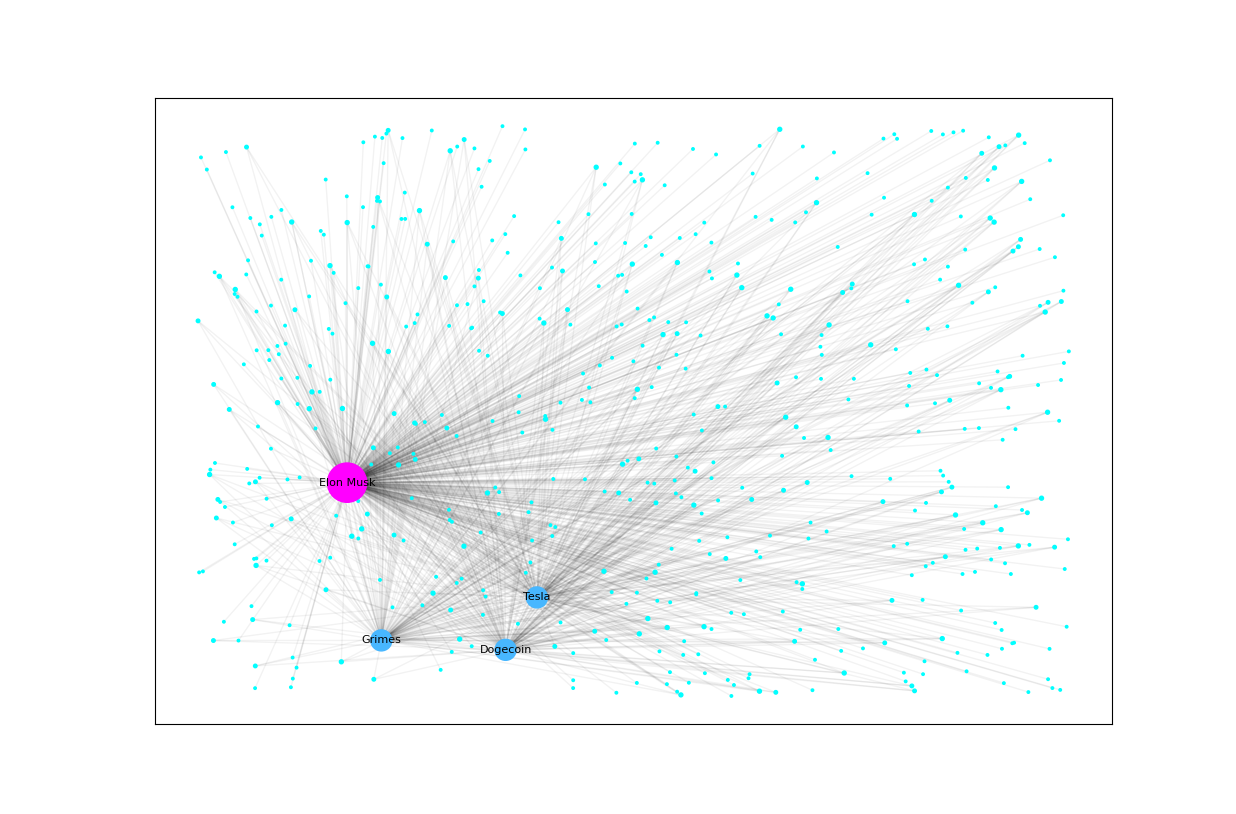
\includegraphics[width=15cm]{Images/elon_graph.png}
    \centering
    \caption{All the circles represent nodes or users in this Twitter network. The edges between the nodes denote follows.
     The red node is a single user in the Twitter network following Tesla, Dogecoin, and Grimes (denoted by the red edges), but no others. The 
    red user receives all tweets and retweets from Tesla, Dogecoin, and Grimes. This user may retweet these messages
    outside the network potentially bringing in more users to the network. Note the red node and its adjacents are isomorphic to, $S_3$ or $H4$.}
\end{figure}


Twitter's status as a complex network aside, the platform is also notable for its position among social networks not only for its size,
but also its influence on culture and politics. During the 2016 election, a survey of
thirty million tweets from two million users, linked articles that were found to be spreading
false information. Moreover, this information spread based on community structure within an inclusive left-right
influencer network. Twitter is cliquey and the communities form around 
shared interests. In online communities where exposure to the same memetic theme occurs frequently, 
facts and rumors may spread easily and quickly \cite{bessi}.

Twitter also has substantial economic impact. Twitter sentiment is known to precede fluctuations
in the stock market \cite{Bollen2011} and Bitcoin prices \cite{bitcoin}. Only a handful of Twitter users actually have influence, 
although groups of people could theoretically be enough to influence market prices \cite{stonks}.
Elon Musk is one such person who, as of March 2021, has influenced multiple markets driving Tesla's share
price up and down \cite{elontweet}, as well as causing jumps in cryptocurrency prices  \cite{elontweet2} \cite{dogecoin}. Musk 
is as of 2021, the forty-third largest Twitter account giving him much more influence than the vast majority of users.

Twitter's suitability as a subject of network science is clear. The users and follows (and retweets) are naturally 
described in by vertices and edges. One can generate networks from Twitter in a two ways.
 First, there are the user accounts which are linked to one another through 
followers and follows, in-degrees and out-degrees. One can also construct networks
of tweets and retweets as discussed in chapter 4. A user posts a message, which is  
retweeted by a portion of their followers, which is then again retweeted by a portion of their followers.
 It is this latter case we will consider in the Thij model.

\chapter{Motifs}
\label{section:Motifs}

Motifs are the primary object of interest as a way of characterizing the local structure of a
network. The dynamic motif count indicates the network and the communities within are evolving according to certain rules.
In the context of static networks, the frequency of motifs 
has been shown to highlight system properties in biological networks \cite{biomotif} \cite{bioAlbert}.

Motifs are the fundamental components of complex systems.
The topological structure of complex networks
is tied to the frequency and distribution of motifs. Initially, the counting of 
these motifs was treated as a static problem where the frequencies of motifs affect functions on networks \cite{motifdiscovery}.
As the significance of motifs becomes more apparent authors have begun examining the emergence of motifs 
via temporal edges \cite{temporalmotifs}. Our motifs will
act as a vector of features characterizing the network at each point in time. Before we
examine our specific motifs we must first define common objects of graph theory such as cycles, paths, and stars
which will aid us in understanding the motifs we would like to examine.

\section{Graph Theory}

In the pursuit of counting our particular motifs we require some
ideas from graph theory. There is no reason some of these objects could not be 
motifs on their own. We will count three-cycles, four-cycles, and five-cycles
as motifs themselves, but for this we require the non-simple cycle motifs.
Much of the literature on motifs focuses on directed triangle ($C_3$) motifs \cite{temporalmotifs} \cite{Milo824}, but 
 the motifs described in this thesis are more varied.
Motifs are generally best described by graphs. 

\begin{dfn}
    Let $G = (V,E)$ be a graph with $V$ being a set of vertices (or nodes), 
and $E$, a set of edges. If $v$ is a vertex of $G$ we write $v \in V(G)$.
If $u,v \in V(G)$ and there is an edge between them we 
write $\{u,v\} \in E(G)$
\end{dfn}

Graphs may be directed or undirected. For directed graphs $\{u,v\} \in E(G)$
is taken to mean there exists an edge from $u$ to $v$ in $G$. Undirected meaning the 
edge between $u$ and $v$ to have no notion of direction.

\begin{dfn}
    The adjacency matrix for any graph $G$ with $n=|V|$ vertices is a matrix of size
    $n \times n$. The element $a_{ij}$ is defined to be
    $$
    a_{ij} = 
    \begin{cases}
        1 \quad e_{ij} \in E(G)\\
        0 \quad \text{otherwise}
    \end{cases}
    $$
    \label{def:adjmat}
\end{dfn}

\noindent The adjacency matrix is critical to all of our calculations to come. It renders
any graph amenable to the tools of linear algebra.

\begin{dfn}
\label{def:homomorphism}
We call $f: G \rightarrow H$ a homomorphism,
if $f$ maps endpoints in $G=(V(G),E(G))$ to endpoints in $H=(V(H),E(H))$.
i.e. $ \forall u,v \in V(G) \quad \{u,v\} \in E(G) \Rightarrow \{f(u),
f(v)\} \in E(H)$.
\end{dfn}

\begin{figure}[h!]
    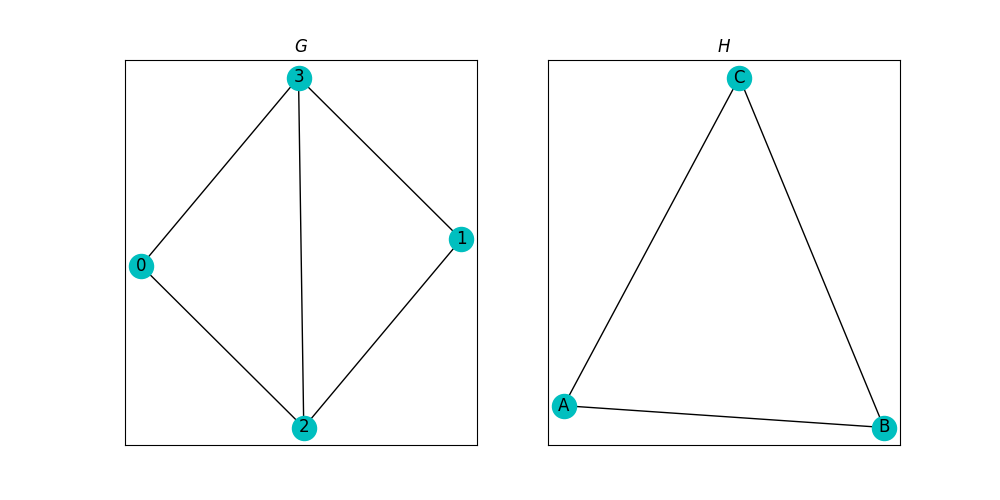
\includegraphics[width=10cm]{Images/graph_homomorphism.png}
    \centering
    \caption{A homomorphism from G to H.}
    \label{fig:homomorphism}
\end{figure}

\noindent  For the example in Figure~\ref{fig:homomorphism} we can define a mapping $f$ such that:

\begin{align*}
    &f(0) = A\\
    &f(1) = A\\
    &f(2) = B\\
    &f(3) = C\\ 
\end{align*}

\noindent $f$ is a homomorphism by the definition presented in definition~\ref{def:homomorphism}. 
We now define particular cases of the graph homomorphism.

\begin{dfn}
    We call $f: G \rightarrow H$ an isomorphism,
 if $f$ is a homomorphism and is bijective.
\end{dfn}

\begin{figure}[h!]
    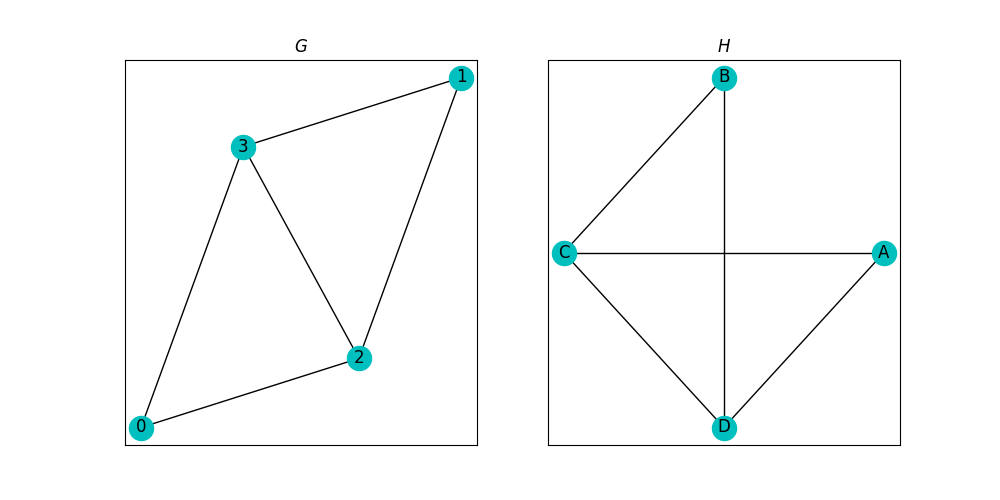
\includegraphics[width=12cm]{Images/graph_isomoprhism.png}
    \centering
    \caption{An isomorphism between $G$ and $H$.}
    \label{fig:isomorphism}
\end{figure}

\noindent We can define an isomorphism $f$ for between $G$ and $H$ in the figure ~\ref{fig:isomorphism} such that:

\begin{align*}
    &g(0) = B\\
    &g(1) = A\\
    &g(2) = C\\
    &g(3) = D\\ 
\end{align*}

\begin{dfn}
    An automorphism is an isomorphism between a graph $G$ and itself. The automorphism 
    is edge-preserving, $\{u,v\} \in G \implies \{f(v),f(u)\} \in G$.
\end{dfn}

\begin{dfn}
    Let $G=(V,E)$ be a graph. We call $G'=(V',E')$ a subgraph if
     $V' \subseteq V \land E' \subseteq E \cap (V' \times V')$. Furthermore we call $G'$
     an induced subgraph of $G$ if for the edges $\{u,v\}$ of $G'$ we have $\{u,v\} \in E, u,v \in V'$.
\end{dfn}

\noindent Induced subgraphs are vital to our understanding of how motifs interact as we add edges or nodes
to a given graph.

\begin{figure}[h!]
    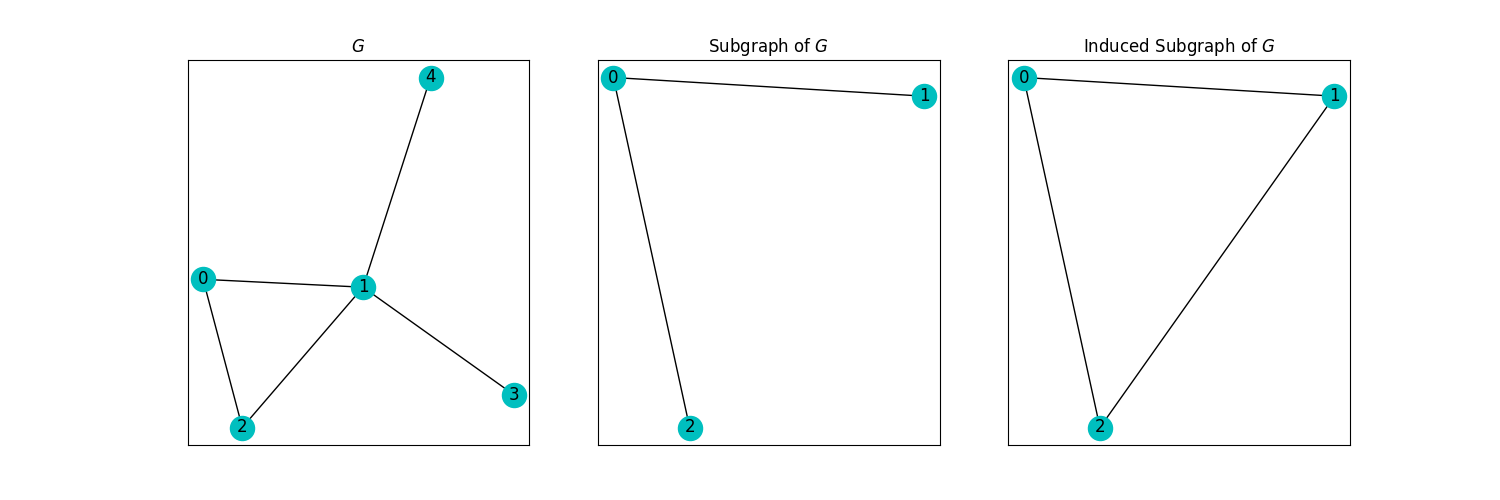
\includegraphics[width=15cm]{Images/subgraph.png}
    \centering
    \caption{Example of subgraphs and induced subgraphs on $G$.}
\end{figure}

\begin{dfn}
    Let $G'' \subset G$ and furthermore let there exist an isomorphism between $G''$ and $G'$. We call
    $G''$ an appearance of $G'$. Provided the number of appearances of $G'$ is greater than some $N$ we call $G'$
    a motif or pattern.
\end{dfn}

\begin{dfn}
    A walk $W = {v_0, e_1, v_1, \dots v_n}$ is a sequence of edges and vertices of $G$ such that
    for $0 \leq k \leq n-1$ the edge $e_i = \{v_k, v_k+1\}$.
\end{dfn}

\begin{dfn}
    A cycle is a walk whose first and last vertex are the same.
\end{dfn}

\begin{figure}[h!]
    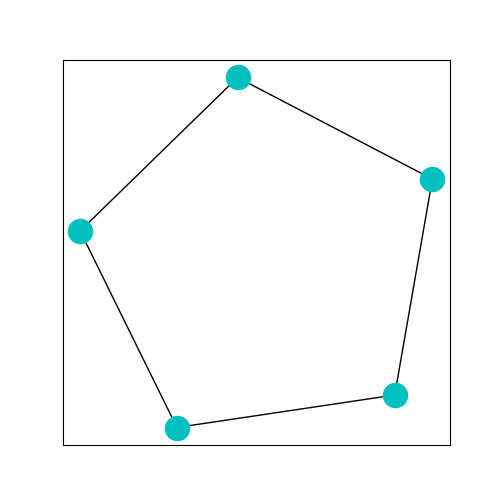
\includegraphics[width=8cm]{Images/Cycle.png}
    \centering
    \caption{A simple cycle of length five.}
\end{figure}

\noindent We will wish to count cycles of length three and four which will be used in the counting of more complicated motifs.

\begin{dfn}
    A bipartite graph is a graph whose nodes may be separated into two disjoint sets $U$ and $V$
    such that there exists an edge between all vertices in $U$ and all vertices in $V$.
\end{dfn}

\begin{figure}[h!]
    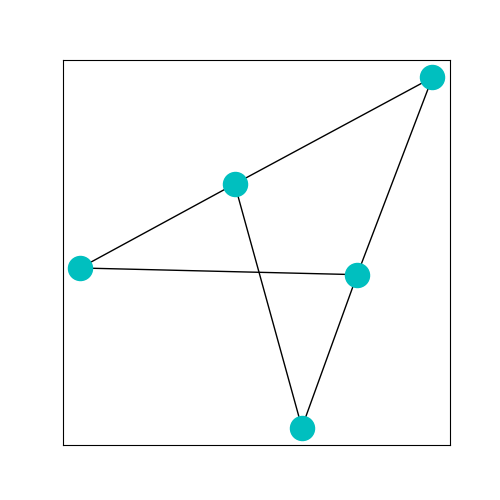
\includegraphics[width=8cm]{Images/Bipartite.png}
    \centering
    \caption{The bipartite graph $K_{2,3}$.}
\end{figure}

\FloatBarrier

\begin{dfn}
    A star $S_n$ denotes the complete bipartite graph $K_{i,k}$. In other words 
    a tree with one internal node, but $k$ branches.
\end{dfn}

\begin{figure}[h!]
    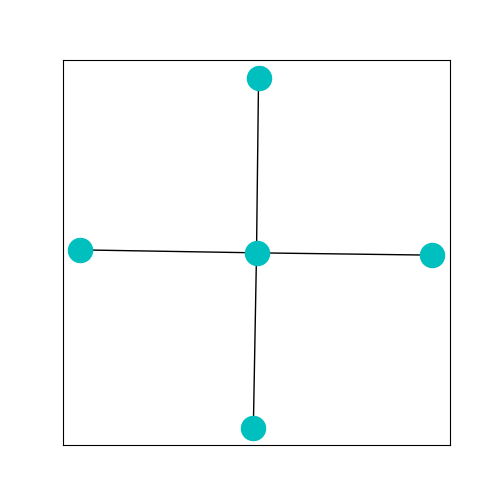
\includegraphics[width=8cm]{Images/Star.png}
    \centering
    \caption{The star $S_4$.}
\end{figure}


The $C3$ and $C4$ motif counts are themselves a measurement of clustering the graph. In fact the
global clustering coefficient defined in chapter one explicitly makes use of the $C3$ count in its 
calculation. The notion of a bipartite graph comes in handy when characterizing some of our motifs, but 
no explicit bipartite graph is counted as a motif. However, the definition of a star graph $S_k$ is very useful, because some of the motif counts increase exponentially
due to the motifs that are generated as a new node or a new edge is added to the $S_k$ graph. 


\newpage

\section{Non-Simple Cycle Motifs}
\label{section:Non-simple Motifs}
We wish to consider the following motifs: $H3$ through $H13$.
These motifs and the ways in which to count them are described in \cite{alon}.


\begin{dfn}
    Let f be a homomorphism between graphs $G$ and $H$. We say that $H$ is a
    homomorphic image of $G$ provided $f$ is surjective.
\end{dfn}

\begin{dfn}
    A graph $H = (V_H, E_H)$ is said to be k-cyclic, for $k > 3$, if it is a
homomorphic image of the cycle $C_k$. The number of different homomorphisms from $C_k$
to $H$ is denoted by $C_k(H)$.  $H$ is $k$-cyclic if and only if $C_k(H) > 0$.
\end{dfn}

These motifs are not simple cycles. For the motifs in figures ~\ref{fig:motifs1} we can classify them according to which cycle 
each graph is a homomorphic image. $H3$, $H4$, $H6$, $H9$, and $H11$ are all six-cyclic. $H5$
is the only five-cyclic graph. However $H5$, $H6$, $H7$, $H8$, $H10$, $H12$, and $H13$ are 
all seven-cyclic.

\begin{figure}[ht!]
    \frame{\includegraphics[width=12cm]{Images/mega_motif.png}}
    \centering
    \caption{The first four non-simple motifs. This set is comprised
    of three-walk ($H3$), a star $S_3$ ($H4$), the star $S_3$ with two vertices
    attached ($H5$), and finally an $S_3$ with two edges added.}
    \label{fig:motifs1}
\end{figure}

% \begin{figure}[h!]
%     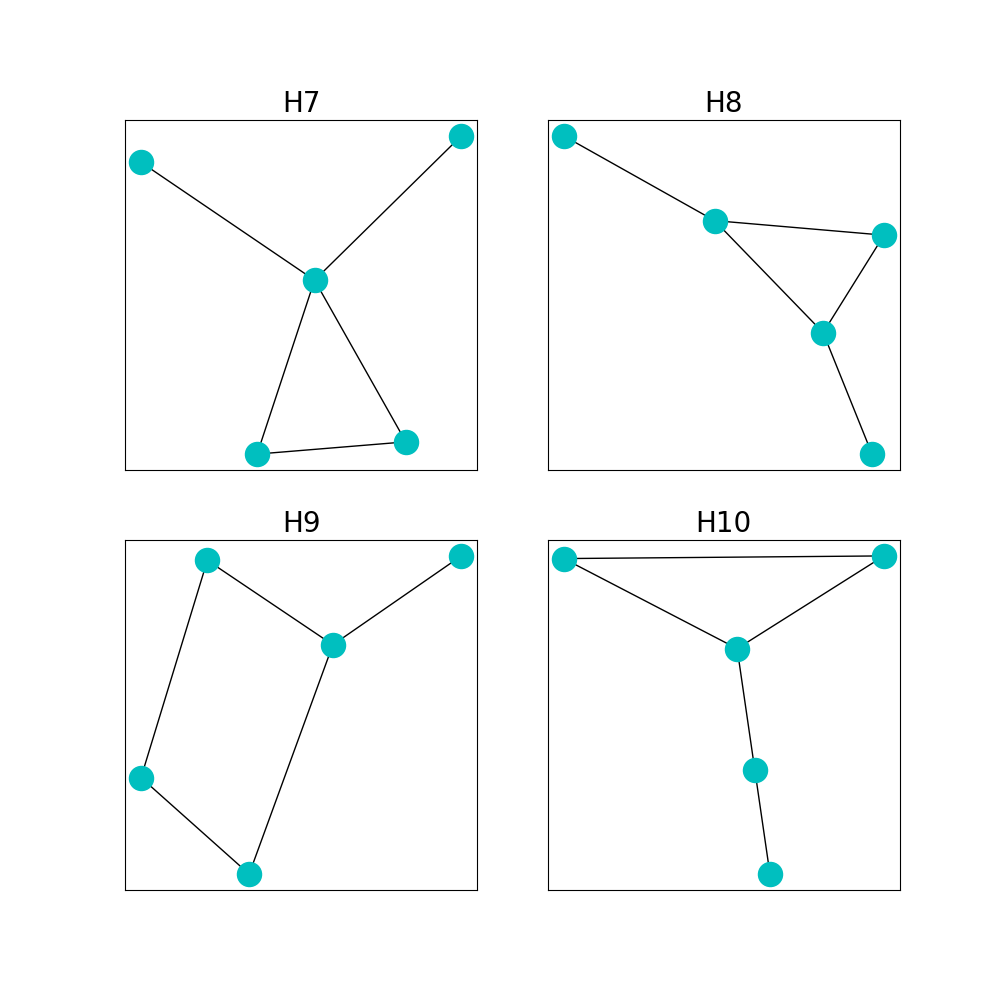
\includegraphics[width=9cm]{Images/motif_set_two.png}
%     \centering
%     \caption{Four more non-simple motifs}
%     \label{fig:motifs2}
% \end{figure}

% \begin{figure}
%     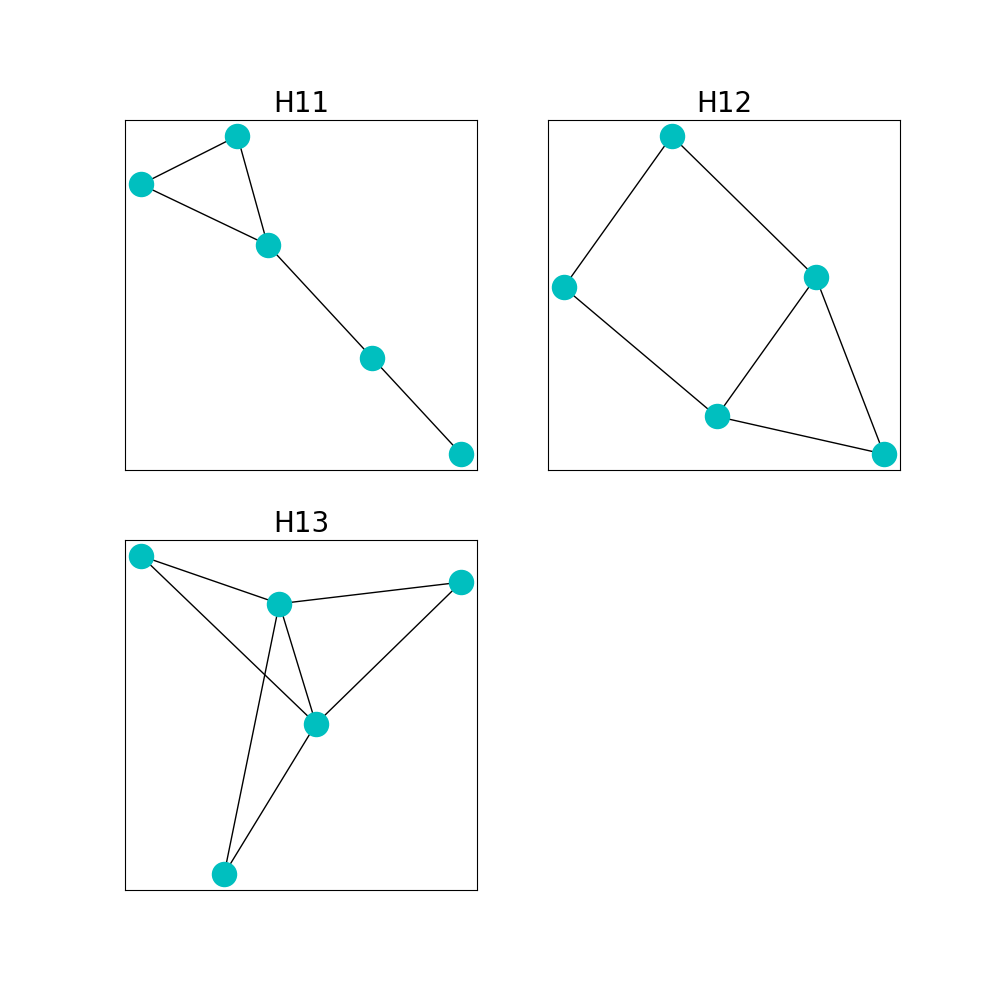
\includegraphics[width=9cm]{Images/motif_set_three.png}
%     \centering
%     \caption{Our last three non-simple motifs}
%     \label{fig:motifs3}
% \end{figure}

\FloatBarrier

\vspace{3mm} 

We will also consider walks of certain sizes as this will be necessary to count appearances at each time. Motif counts can be generated from a network's adjacency matrix in the following ways. Let $A$
be the adjacency matrix of some arbitrary network with greater than four nodes. Let $N_m(A)$ denote 
the total count of motif $m$ in the network. 

\vspace{3mm}

When counting the motifs we let $E$ denote the set of edges in the network, $e_i,j$ denotes a particular edge between the 
i'th and j'th nodes. $d_i$ denotes the degree of the i'th node. $A$ is the adjacency matrix of the
 graph $G$. Finally, $a^{(k)}_{i,j}$ denotes the kth power of the matrix 
element at the i'th row and j'th column of matrix $A$. The formulae for motif counts are as follows:

\newpage

\begin{align*}
    &N_G(C3) = \frac{1}{6} \tr({A^3}) \\
    &N_G(C4) = \frac{1}{8} \left(\tr(A^4) -4\sum^{n}_{i=1} {d_i \choose 2} - 2\sum_{i,j \in E} e_{ij} \right)\\
    &N_G(C5) = \frac{1}{2}\sum_{(i,j)\in E} (d_i - 1)(d_j - 1) - 3 N_{C3} \\
    &N_G(H4) = \sum^{n}_{i=1} {d_i \choose 3} \\
    &N_G(H5) = \frac{1}{2} \sum^{n}_{i=1} a^{(3)}_{ii} (d_i-2)\\
    &N_G(H6)= \sum_{(i,j)\in E}{a^{2}_{i,j} \choose 2 }\\
    &N_G(H7) = \frac{1}{2} \sum^{n}_{i=1} a^{(3)}_{ii} {{d_i-2} \choose 2}\\
    &N_G(H8)= \sum_{(i,j)\in E} a^{(2)}_{ij} (d_i-2)(d_j-2) - 2 N_G(H6)\\
    &N_G(H9) = \sum^{n}_{i-1}(d_i-2) \sum_{j \neq i} {a^{(2)}_{ij} \choose 2 }\\
    &N_G(H10) = \frac{1}{2}\sum^{n}_{i=1}a^{(3)}_{ii} \sum_{j \neq i} a^{(2)}_{ij} - 3 N_G(C3)- 2N_G(H5) -4N_G(H6)\\
    &N_G(H11) = \sum^{n}_{i=1} {\frac{1}{2}a^{(3)}_{ii} \choose 2} - 2N_G(H6)\\
    &N_G(H12) = \sum_{(i,j)\in E} a^{(2)}_{ij} a^{(3)}_{ij} - 9N_G(C3) -2N_G(H5)-4N_G(H6)\\
    &N_G(H13) = \sum_{(i,j)\in E} {a^{(2)}_{ij} \choose 3}\\
\end{align*}

We want to understand how each of the motif counts affect another given a certain event occurs
in any of the simulations. Some motifs contain induced subgraphs of the others and simple changes
to a motif may cause a combinatorial effect or multiplicative of new motifs appearing.

\chapter{Barabási–Albert Model}
\label{section:BA model}
The early models of networks failed to capture the characteristics that appear in empirical data. An
early model proposed by Paul Erdős and Alfréd Rényi, appropiately called the Erdős–Rényi model, generates
graphs of fixed node counts where each has the same probability of existing. 
Réka Albert and Albert Barabási recognized the Erdős–Rényi model 
was incapable of modeling real-world phenomena, because the Erdős–Rényi model does not add
in new nodes or edges through a temporal process. All edges in the Erdős–Rényi model are added at random
according to a parameter value, but complex networks are not entirely random.
They conform to rules guiding the hand of chance. 
In three key areas the real networks differed from those
of the Erdős–Rényi graph \cite{barabasi2016network}.
 First, the real networks often had degree distributions 
that are not explainable according to a Poisson distribution.
 The tail of the Poisson
distribution did not allow for the observed degree distributions.
Second, real networks had a sizable largest connected component - a large cluster 
of nodes inside the network, forming a hub of activity.
 Finally, the local clustering coefficient of most networks
decreases as the node degree decreases,
 but is independent of overall graph size. For the Erdős–Rényi model
the local clustering coefficient is independent of the node degree and the average local clustering coefficient
depends on the size of the whole network \cite{barabasi2016network}.

Réka Albert and Albert Barabási developed a theory of complex networks 
encompassing those networks we find common in practice. They contended that ultimately the 
Erdős–Rényi model failed to account for the growth of networks over time. The addition
of new nodes and new edges into the network generated the networks' defining characteristics.
Edges were also found to obey the preferential attachment
mechanism which ascribes probabilities of attachment based upon the relative degree of the nodes in a network. 
This model was found to simulate scale-free networks well as the model's
degree distribution is described by a power-law. 
A network is scale-free provided the degree distribution of the network follows a power law. 

The fraction of nodes $P$ having $N$ nodes attached for large values of $k$ is 

$$
P(N) \approx k^{-\gamma} , \quad 2< \gamma <3
$$
%%%%%% Left off editing here

We first begin at $t=0$ by initializing a $m$ number of nodes and randomly distribute a number of edges between them
according to a uniform distribution. Then at each time-step $t > 0$, we introduce a new node 
and a $k$ number of edges between that node and existing nodes. We assign probabilities of attachment via the
 probability distribution:

$$
P(n) = \frac{d_n}{\sum^{N}_{i=1} d_i}
$$

\noindent where $d_i$ is the degree of the i'th node and $N$ is the total number of nodes at $t-1$. This means 
that nodes which have a high degree are probabilistically more likely to be attached to be new nodes. 


\begin{figure*}[h!]
    \includegraphics[width=16cm]{Images/pref_attach_1_counts.png}
    \centering
    \caption{This Barabási–Albert model is initialized with $m=8$ uniformly connected nodes.
    At each time-step a new node enters and is attached to $k=1$ nodes in accordance
    with the preferential attachment mechanism. Only those motif counts which have a node
    of degree one can increase given $k=1$.}
    \label{fig:BA1}
\end{figure*}


\begin{figure*}[h!]
    \includegraphics[width=14cm]{Images/graph_stats_pref_attach_8_1_300.png}
    \centering
    \caption{Statistics characterizing the development of the Barabási–Albert model for $k=1$.
    Edges and nodes grow linearly, the number of edges being added is $k$-times per time-step. We also 
    see as Barabási noted, the edge density decreases asymptotically.}
\end{figure*}


\begin{figure*}
    \includegraphics[width=14cm]{Images/final_pref1_centrality.png}
    \centering
    \caption{The Barabási–Albert model for $k=1$ at the final time-step.}
\end{figure*}

\begin{figure*}[h!]
    \includegraphics[width=16cm]{Images/pref_attach_2_counts.png}
    \centering
    \caption{This Barabási–Albert model is initialized with $m=5$ uniformly connected nodes.
    At each time-step a new node enters and is attached to $k=2$ nodes. We see that different motifs
    correlate for the $k=2$ simulation and other motifs like $H5$ can be generated.}
    \label{fig:BA2}
\end{figure*}

\begin{figure*}[h!]
    \includegraphics[width=14cm]{Images/graph_stats_pref_attach_10_2_300.png}
    \centering
    \caption{Statistics characterizing the development of the Barabási–Albert model for $k=2$.
    Edges and nodes grow linearly, with m edges added each time-step. As Barabási noted, the edge density decreases asymptotically. The histogram at
    the final time also shows that the vast majority of nodes, approximately 220, have two or three attachments
    while three vertices have a degree greater than $35$.}
\end{figure*}

\begin{figure*}
    \includegraphics[width=14cm]{Images/final_pref2_centrality.png}
    \centering
    \caption{The Barabási–Albert model for $k=2$ at the final time-step.}
\end{figure*}

The Barabási–Albert model exhibits a few characteristics that differentiate it from the 
Erdős–Rényi model. If we consider its diameter, the maximum distance in the network
for $k>1$ and sufficiently large time we can write the diameter 

$$\text{diam}(G) = \frac{\ln(N)}{\ln(\ln (N))}$$

The diameter grows slower than $\ln(n)$ meaning the graph's diameter grows slower than that of the 
Erdős–Rényi model. We can also examine the clustering coefficient of the model. 
The clustering coefficients for the preferential attachment model grows according to \cite{klemm_2002}

$$
C(G) = \frac{(\ln (N))^2}{N}
$$

This differs from the Erdős–Rényi model by the term $(\ln (N))^2$,
which increases the clustering coefficient for large $N$. Still both measures
decrease, asymptotically approaching zero. 
From this result we see Barabási-Albert network is locally more clustered than a random network for all $N$ \cite{barabasi2016network}.

Motif counts in the Barabási–Albert model are dependent upon the initialization of the $m$ nodes 
and the choice of $k$. For example, in $k=1$ the model cannot complete any new cycles. If the
intial graph at $t=0$ does not contain any $C_3$ or $C_4$ appearances then any motif 
which has an induced subgraph isomorphic to $C_3$ or $C_4$ cannot appear. The BA model 
for $k=1$ can only attach nodes to the existing  $C_3$ or $C_4$ appearances and in that 
way generate new $H7$'s, $H8$'s, $H9$'s. 

The $k=2$ BA model is capable of generating those new $C_3$ and $C_4$ appearances in the network 
quite easily. The radically changes the motif composition as we can see in figures BLANK.

The model is a good candidate to compare to the Thij model, given that the Thij model incorporates
a preferential attachment mechanism itself. The thij model is more complex and they study of how motifs interact
in the Thij model is, in comparison, much more difficult. The Barabási–Albert model 
represents a simpler, non-trivial model which is widely acknowledged as a useful tool
for understanding networks across a variety of disciplines. We should note the 
limitations to the Barabási–Albert model. The nodes and edges are restricted to growing linear which
may fail to capture certain phenomena that appear empirically. The model is also incapable
 of removing nodes, a point on which Barabási himself has elaborated. The following model
 does account for these first of these limitations at the cost of increased complexity.

\chapter{Twitter and the Thij Model}
\label{section:Thij model}
The Thij model is a particular random graph that seeks to model the development of a Twitter network 
 \cite{thij}. Twitter offers a platform where a user may post a message
to all of their followers' feeds. Those followers may then ignore, like, reply (comment), or retweet (quote tweet) that message. In the
instance they choose to retweet the message, that message is then posted to their respective feed and their
set of followers now have the opportunity to then retweet that same message. It is easy to infer that if a 
message has received a significant number of retweets 
 then the message is more likely to be seen, and thus
retweeted again. Intuitively, we suspect a preferential attachment mechanism driving the popularity of the most popular tweets.

A user can retweet different original messages at different times meaning edges are generated between
existing nodes in the network. Accounting for this one can produce
a model better suited to Twitter than the Barabási–Albert model described in chapter 3.

We wish to simulate a network of retweets. There are the original message nodes from users $u_i$ and retweets from users $v_i$. All users
are capable of retweeting or posting original messages, but for clarity we make a distinction between the posts of original messages and retweets.
 The set of all descendants of $u_i$ (all retweets of the original message and retweets of retweets) and the edges between them
we loosely call a message tree. $v_i$ may be a simple retweet or a quote tweet meaning $v_i$ may reasonably retweet $v_k$ who may have added commentary to the original message.
 The simulation starts with an initial message node from user $u_{0}$ at time $t=0$. There is now the possibility of three events: $T1$,
$T2$, and $T3$.

\vspace{3mm}
$\pmb{T1}$: A new message node from user $u_t$ appears.

\vspace{3mm}
$\pmb{T2}$: A user $v_k$ enters the retweet network and retweets an existing user, either a $u_i$ who has posted an original message or $v_k$ with $i \neq k$ who
has simpley retweeted another user in the network. This user $v_k$ retweets an original message node $u_i$ with 
probability $q$ and any other node with probability $\frac{1-q}{N}$, $N$ being the total number of nodes in the network.

\vspace{3mm}
$\pmb{T3}$: An existing user $v_i$ retweets another existing user $u_i$ or $v_k$. Once again the retweeter retweets a message node with probability 
$q$ and all other message or retweet nodes with probability $\frac{1-q}{N}$.

We must also note that, generally, there will be multiple message nodes in the retweet graph, and thus,
 we have to decide for any given event
which particular message node should be assigned the $q$ probability.
 Here we introduce a preferential attachment mechanism. At any time $t$,
given a $T2$ or $T3$ event occurring, the probability of a particular message node being chosen is almost the
same mechanism described in the Barabási–Albert model. Instead, a message node is chosen
by its total descendants and not by the degree of the message node itself. In essence, a message node
is selected based upon the number of those who have retweeted the message and all those who have retweeted
retweets of that message.


We now must assign probabilities of $T1$, $T2$, and $T3$ events. Let $\lambda \geq 0$ and $1 \geq p \geq 0$,
\begin{align*}
    &P(T1) = \frac{\lambda}{1 + \lambda} \\
    &P(T2) = \frac{p}{1 + \lambda} \\
    &P(T3) = \frac{1-p}{1 + \lambda} \\
\end{align*}


\begin{figure*}
    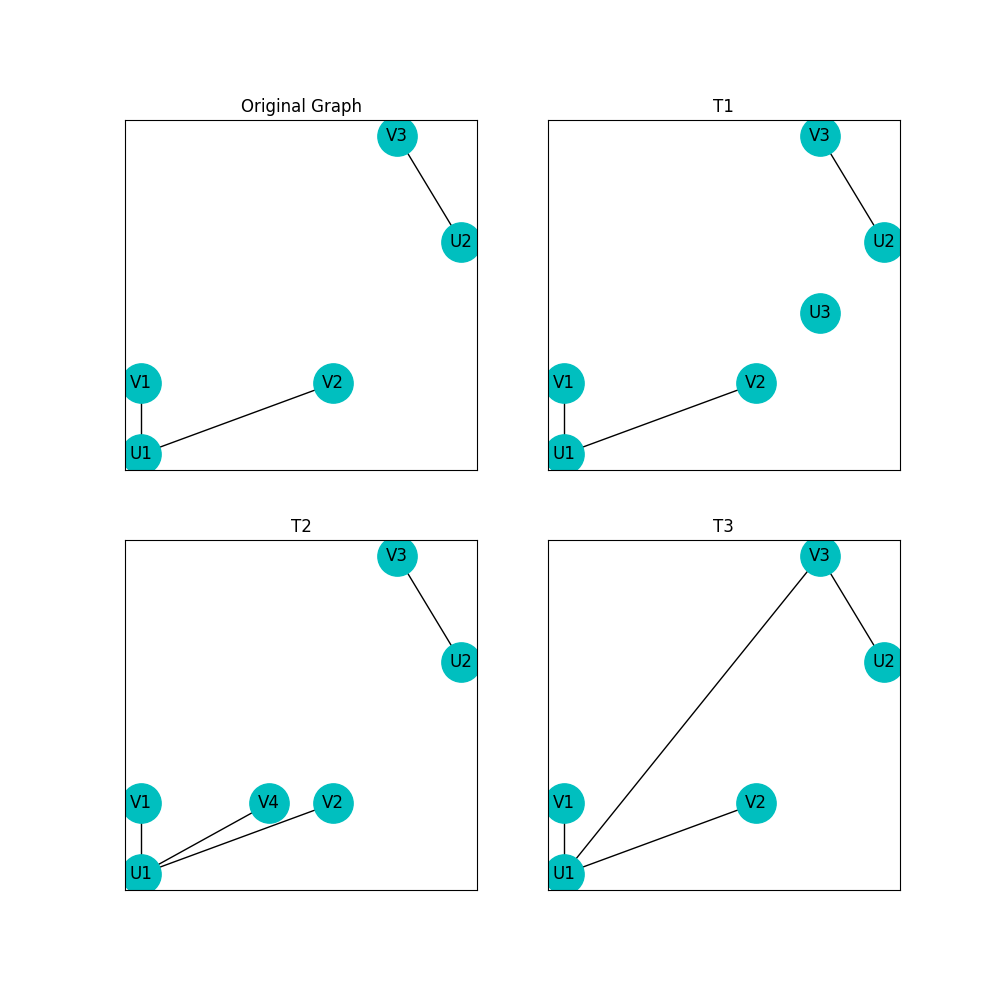
\includegraphics[width=12cm]{Images/events.png}\
    \centering
    \caption{We see the $T1$, $T2$, and $T3$ events on a simple graph. In the $T1$ case 
    we see a new message node $U3$ appears. It has yet to be connected to anything at all. In $T2$
    we see a new node $V4$. This is a retweet of the message $U1$. Finally in the last plot we see
    a $T3$ event. Here the user $V3$, who has already retweeted $U2$, now retweets message $U1$.}
\end{figure*}

Our choices of $\lambda$ and $p$ will drastically affect the dynamics of the graph, as well as the subgraph motifs that make
up its structure. We want to consider a series of cases for different probabilities allowing us to make informed predictions about the development
of the graph over time.

% \begin{figure}[h!]
%     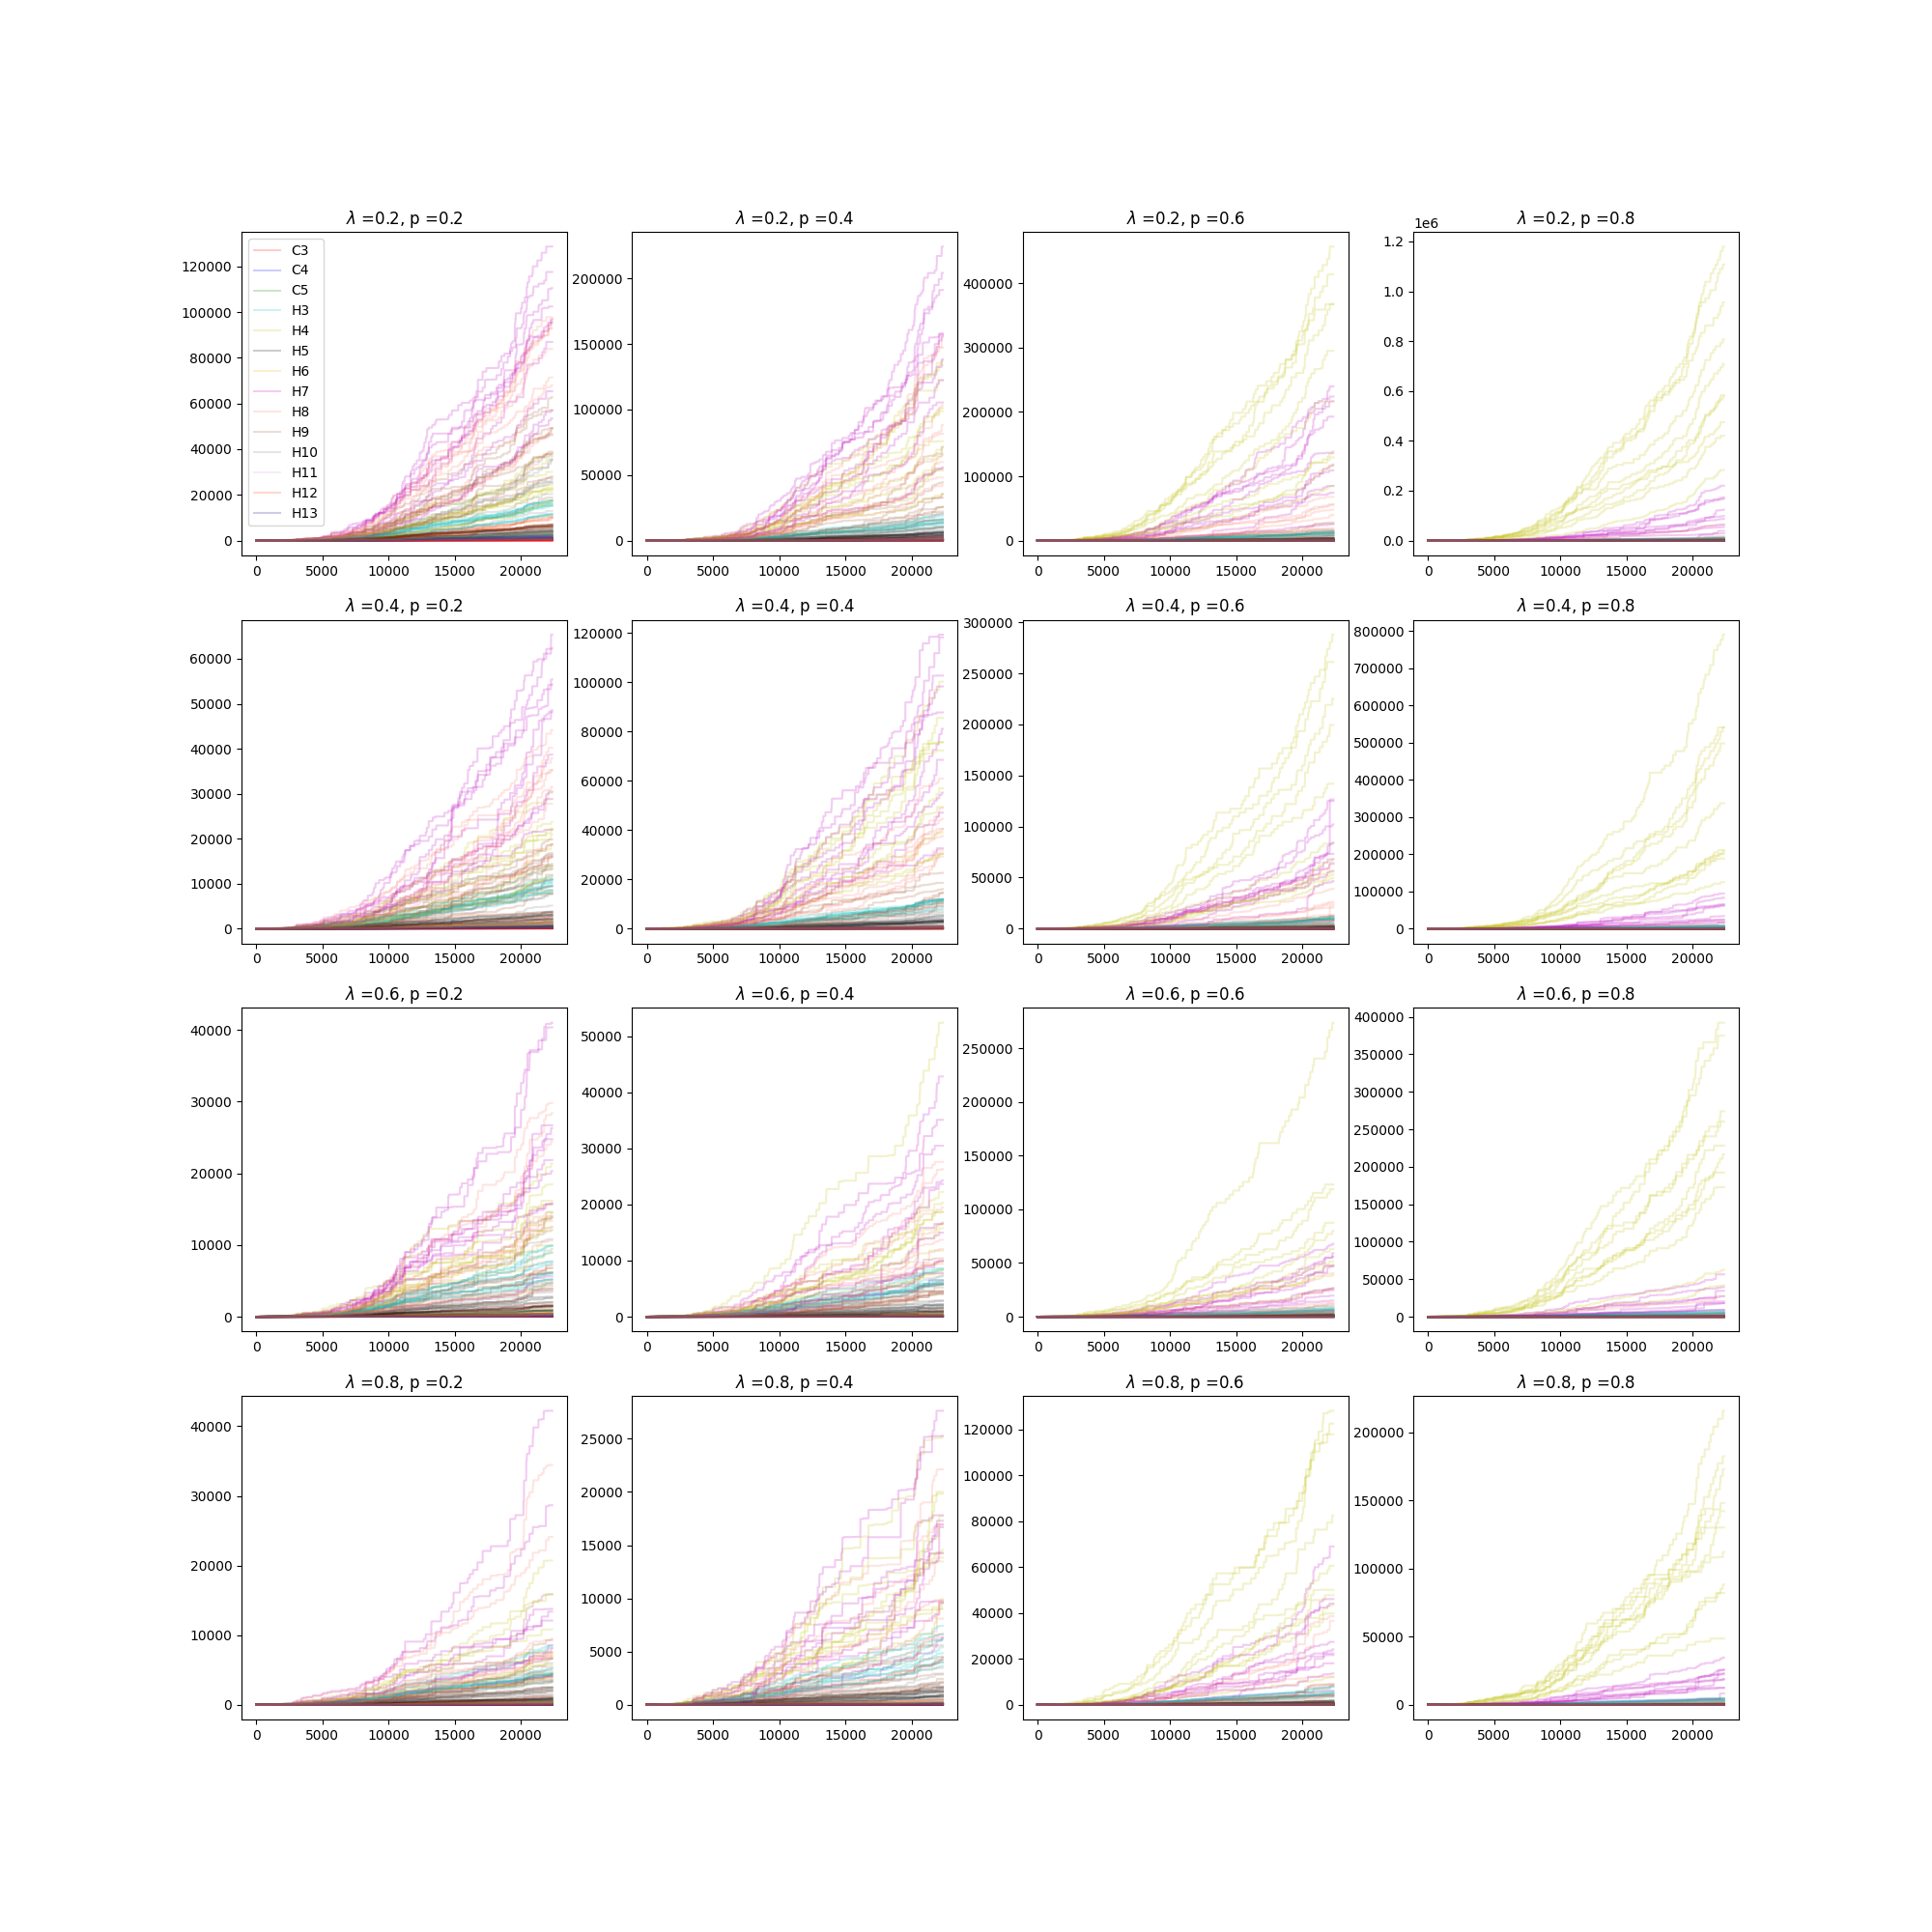
\includegraphics[width=10cm]{Images/full-sims-graph_mid_set.png}
%     \centering
%     \caption{Above we see motif counts for varying parameters. The scales on the y-axis differ widely,
%     but we also see prominence of different motifs dependent upon the parameter choices. 
%     Some parameters lead to large, induced star subgraphs, while others may lead to
%      highly clustered communities that share a few connections between their nodes.}
% \end{figure}
% \newpage

The motif counts for various parameters help demonstrate the differences in scale 
and structure which arise from different probability distributions. 
considering $1>\lambda>0.5$ and $1>p\gg0.5$, we see an increased chance of adding
many new root messages, but still good possibility of introducing a new node with a new edge, but a decreased possibility of 
adding in only new edges. For an example of the resulting motif counts we can look to figure~\ref{fig:thij0808}. 
What about the case $0 < \lambda \ll 0.5$ and $1 > p \gg 0.5$? Now the probability distribution is such that adding a new node
with an edge is the most likely outcome. These parameter choices combines with the superstar parameter $q=0.9$ means that $T2$ and $T3$
attachments are very likely to target the root message node. Below we see the resulting star pattern in the motif counts in figure~\ref{fig:thij0208}
and the end-result in figure ~\ref{fig:network0208}.

The preferential attachment mechanism then encourages
 an induced subgraph $S_{k}$ to form with $k\gg 1$.
 For any $k \gg 3$ $S_{k}$
itself has many appearances of $H4$ and for every increase in $k$ we see an increase in the probability
of yet another increase in $k$.

Next, consider $1>\lambda>0.5$ and $0.5 \gg p > 0$. Here the $T1$ event should dominate the dynamics
 with many new message nodes introduced to the overall retweet network. However, in this scenario we have
 a greater liklihood of $T3$ events. This means those nodes without connections are likely to become connected to other message nodes. In figures
 ~\ref{fig:thij0802} and ~\ref{fig:network0802} we can visualize the motif development and the overall network. Looking at the final time degree
 distribution in figure~\ref{fig:stats0802}, we see that the majority of nodes are still unconnected.

Last we consider the case when $0.5 > \lambda > 0$ and $0.5 \gg p > 0$. In this case, it is the $T3$ event
 expected to be the most prevalent. For these parameter values, we see in figure ~\ref{fig:thij0202} the first four greatest motif counts almost 
 everywhere in order are $H8$,$H10$,$H9$, and $H7$. The $T3$ mechansim allows for more $C_3$'s and $C_4$'s to form within the network.


% \clearpage

\section{$\lambda=0.2$, $p=0.2$}

\begin{figure*}[h!]
    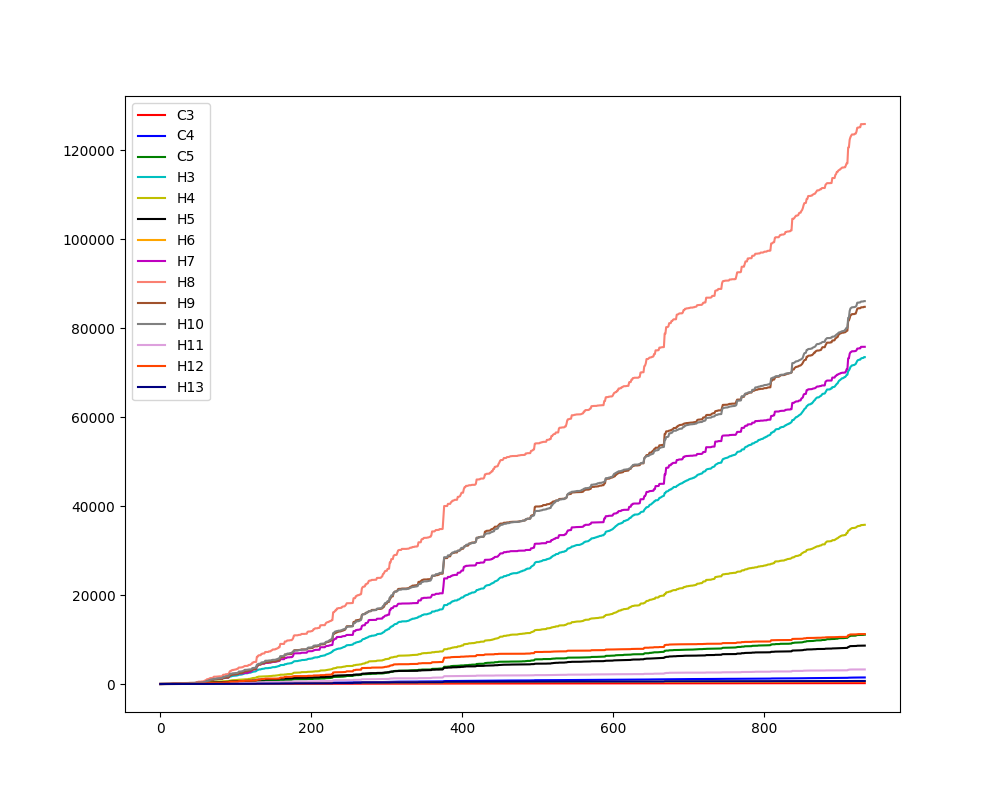
\includegraphics[width=15cm]{Images/twitter_sim_for_stats_3_0.2_0.2.png}
    \centering
    \caption{Here we see that $H8$'s lead with $H9$'s and $H10$'s. These motifs are
     closely correlated with one another throughout the time series. $H7$'s
    and $H3$'s have the next highest counts where $H7$ movement prima facie
    appears to correlate with $H8$ counts, while $H3$ counts steadily increases throughout time.}
    \label{fig:thij0202}
\end{figure*}

\begin{figure*}[h!]
    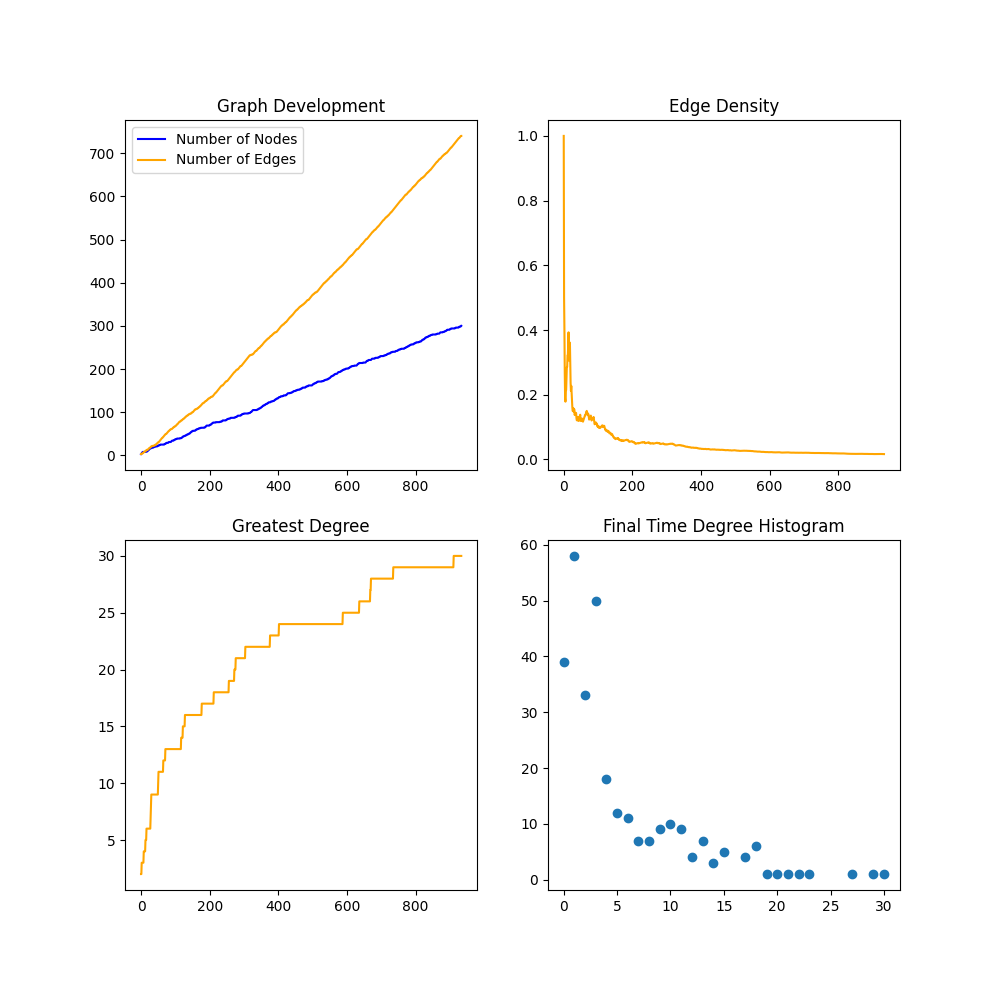
\includegraphics[width=14cm]{Images/twitter_sim_stats_3_0.2_0.2.png}
    \centering
    \caption{Compared to the Barabási–Albert model it's obvious neither edge count nor node
     count grow strictly linear at each time-step. The edge density still tends toward
     zero, although a $T3$ event would amount to an increase in edge density. Finally, we 
    see a final time degree histogram that is similar.}
\end{figure*}

\begin{figure*}[h!]
    \includegraphics[width=14cm]{Images/final_Thij_centrality_0202.png}
    \centering
    \caption{The network for $\lambda=0.2$, $p=0.2$ at the final time-step.}
\end{figure*}

\clearpage

\section{$\lambda=0.8$, $p=0.2$}

\begin{figure*}[h!]
    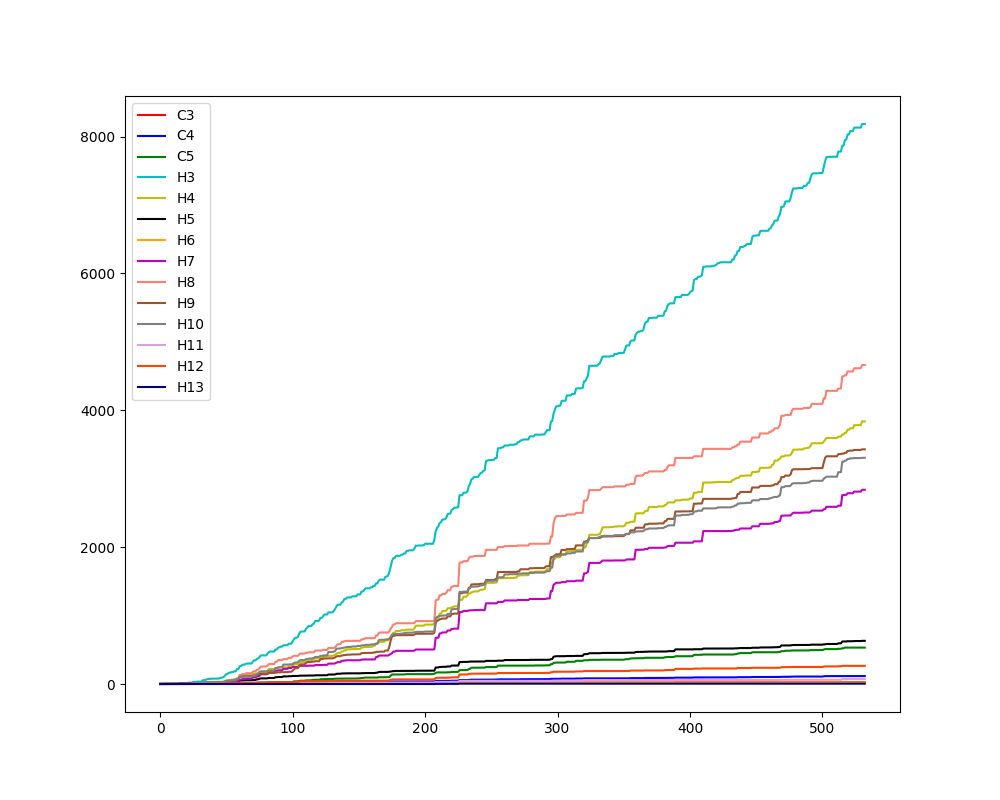
\includegraphics[width=15cm]{Images/twitter_sim_for_stats_3_0.8_0.2.png}
    \centering
    \caption{For high $\lambda$ we see many new message nodes appear ($T1$ events), but
    with low $p$ we should see many $T3$ events. $H3$ motifs are the most prevalent
    followed by $H8$'s and $H4$'s.}
    \label{fig:thij0802}
\end{figure*}

\begin{figure*}[h!]
    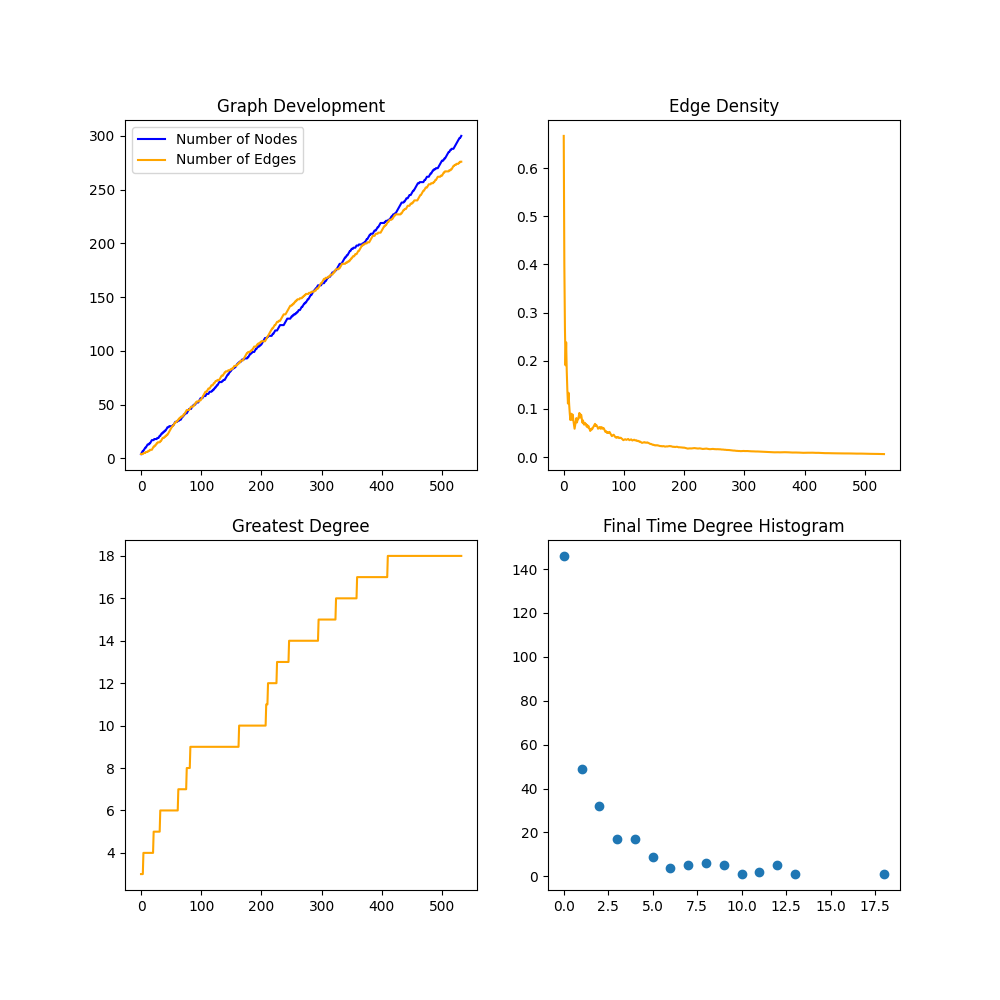
\includegraphics[width=14cm]{Images/twitter_sim_stats_3_0.8_0.2.png}
    \centering
    \caption{The edges and nodes travel tightly together with roughly a ratio of 
     one-to-one. Here we see many, many nodes unattached with degree zero.
    For those that are attached we do see a power law describing degree distribution, but one that is not quite
    as strong as those found in other simulations.}
    \label{fig:stats0802}
\end{figure*}


\begin{figure*}[h!]
    \includegraphics[width=14cm]{Images/final_Thij_centrality_0802.png}
    \centering
    \caption{The network for $\lambda=0.8$, $p=0.2$ at the final time-step.}
    \label{fig:network0802}
\end{figure*}

\clearpage

\section{$\lambda=0.2$, $p=0.8$}

\begin{figure*}[h!]
    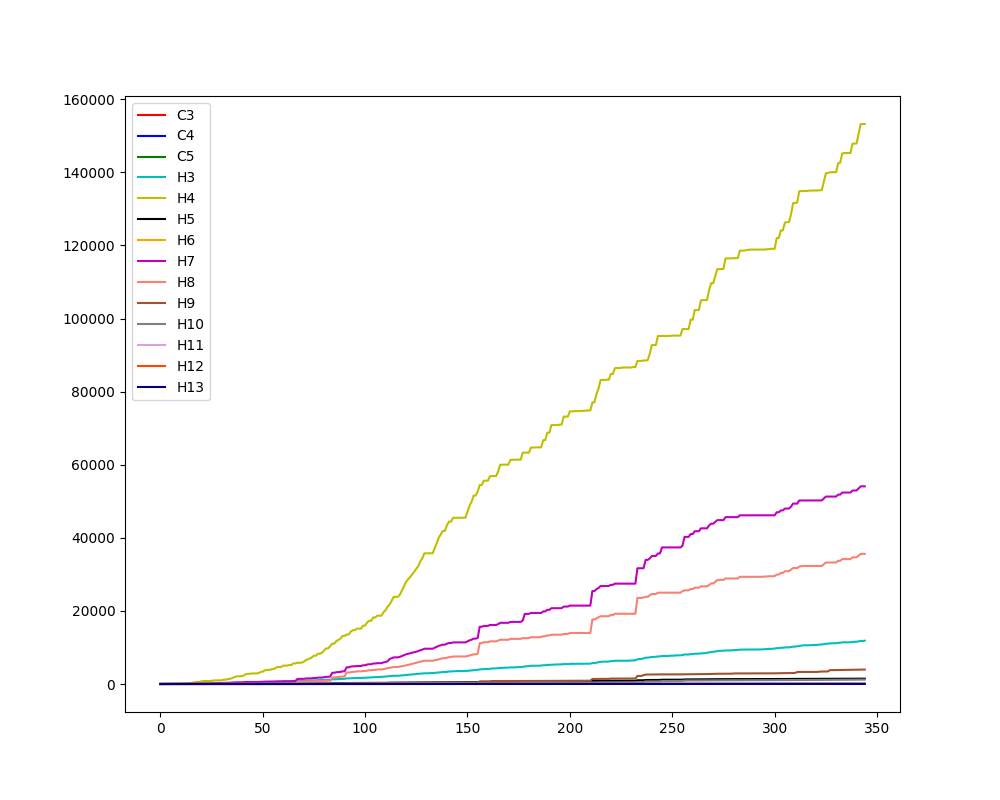
\includegraphics[width=16cm]{Images/twitter_sim_for_stats_3_0.2_0.8.png}
    \centering
    \caption{Small $\lambda$ decreases the likelihood of new message nodes appearing, but 
    high $p$ means a greater likelihood of $T2$ events which we speculate lead to a large
    count of $H4$'s. $C_3$'s exist around the center where all these $H4$'s
    overlap. Although $C3$'s are not prevalent here, a combinatorial effect generates 
    many $H7$'s and $H4$'s.}
    \label{fig:thij0208}
\end{figure*}


\begin{figure*}[h!]
    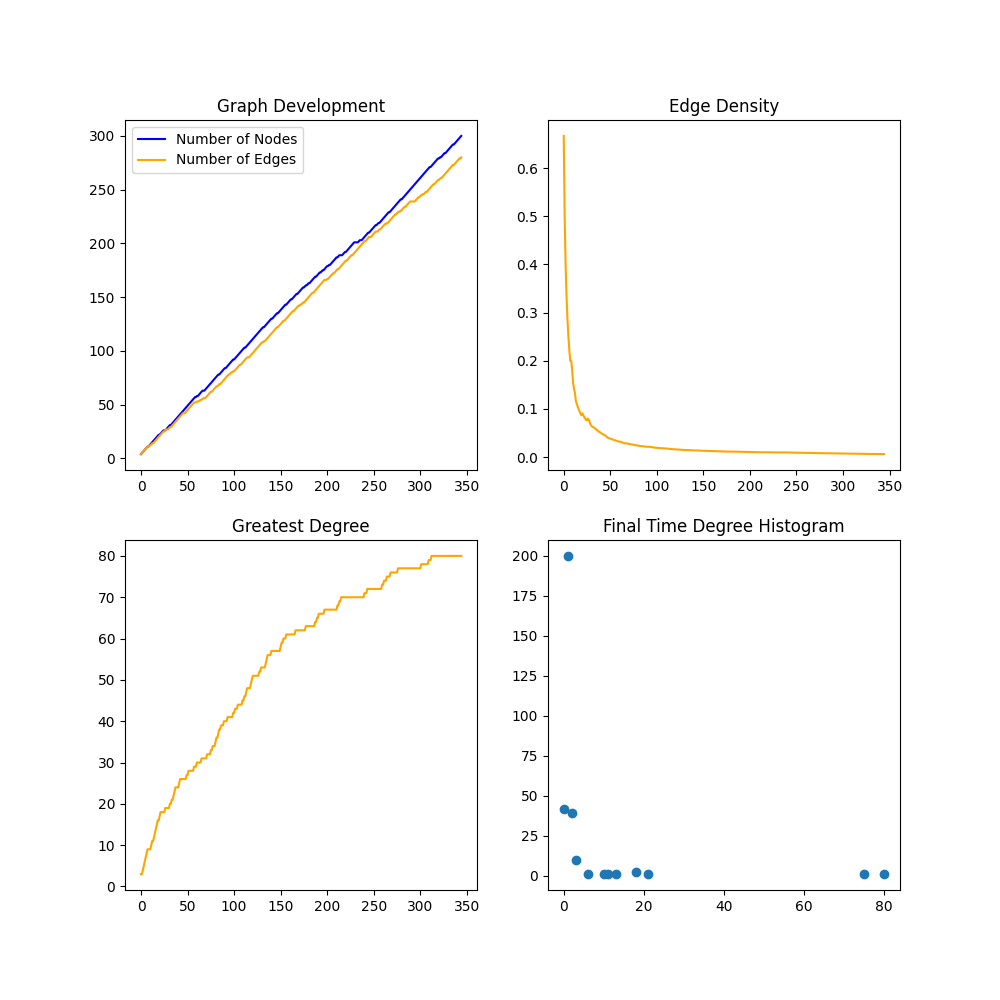
\includegraphics[width=14cm]{Images/twitter_sim_stats_3_0.2_0.8.png}
    \centering
    \caption{Here, we see two nodes with degrees greater than seventy,
    but an abundance of nodes with only one or two connections. This suggests
     a couple (or several) large star graphs focused around two heavily connected nodes. This 
    would produce the abundance of $H8$'s in the motif counts.}
    \label{fig:twittersim28}
\end{figure*}


\begin{figure*}[h!]
    \includegraphics[width=14cm]{Images/final_Thij_centrality_0208.png}
    \centering
    \caption{The network for $\lambda=0.2$, $p=0.8$ at the final time-step.}
    \label{fig:network0208}
\end{figure*}

\clearpage

\section{$\lambda=0.8$, $p=0.8$}

\begin{figure*}[h!]
    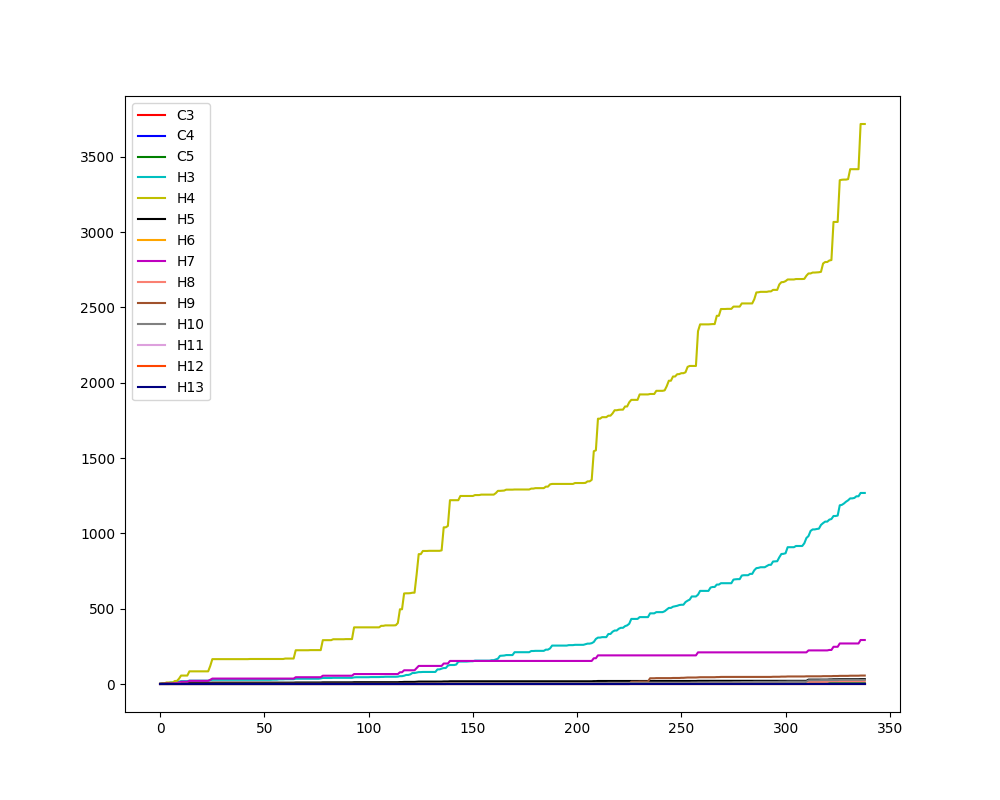
\includegraphics[width=16cm]{Images/twitter_sim_for_stats_3_0.8_0.8.png}
    \centering
    \caption{Here, like the simulation directly in figure ~\ref{fig:twittersim28}, we see a prominence of $H4$'s. The scales
    however are separated by several orders of magnitude. Particular to this simulation
     we have a relatively high count of $H3$'s. We can explain the difference in magnitude
     due to many $T1$ events introducing many nodes, but the occurrence of $T2$ events 
     is still sufficient to make $H4$ the motif of highest count.}
     \label{fig:thij0808}
\end{figure*}

\begin{figure*}[h!]
    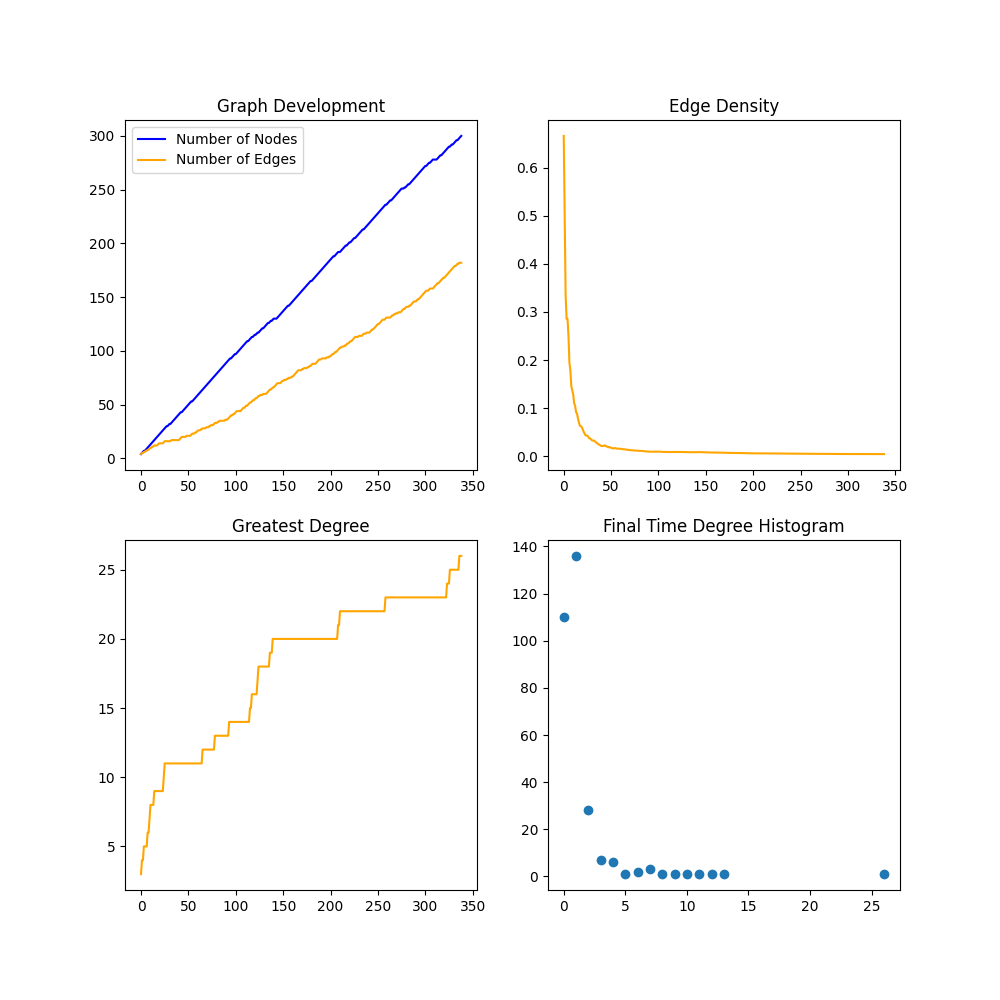
\includegraphics[width=14cm]{Images/twitter_sim_stats_3_0.8_0.8.png}
    \centering
    \caption{This Twitter simulation produces many more nodes than 
    edges, because of the frequency of $T1$ events. The vast majority of nodes only 
    have degrees of one or two, while we see a single node with 25 connections.
    This might suggest many small clusters of nodes with a single larger
    cluster around a single message node.}
\end{figure*}


\begin{figure*}[h!]
    \includegraphics[width=14cm]{Images/final_Thij_centrality_0808.png}
    \centering
    \caption{The network for $\lambda=0.8$, $p=0.8$ at the final time-step.}
\end{figure*}

\clearpage

The dynamics and end state of the network vary across parameter choices.
Given greater $p$ values and smaller $\lambda$ values, the degree distribution will obey stronger
power laws. The ratio of edges to vertices for the Twitter model varies much more than the Barabási-Albert model
which is to be expected given the probabilistic nature of how many edges may be added in a given turn (0 or 1) compared
to the given $m$ of the Barabási–Albert model. This affects not only the strucutre of the network, but the time scale 
over which the network grows.

Each graph spans over \textit{very} different
time frames. Each graph was allowed to grow to a maximum of three-hundred nodes, same as the
sampled Barabási–Albert run, before ending the simulation. Ending the simulation with a size
threshold makes a comparison of the topology of the networks more feasible. For $\lambda=0.2$ and $p=0.8$, the model was able to reach 
three-hundred nodes very quickly, in approximately three-hundred time-steps, whereas for $\lambda=0.2$, $p=0.2$ it took nearly a thousand time-steps. This is consequent of how $\lambda$ controls how often a new node enters without a new edge and
$p$ controls the rate at which new nodes are added without attached edges or if only new edges are introduced. 

\chapter{Barabási–Albert Model Motif and Thij $T2$ Event Motif Dynamics}

To gain insight into graph dynamics, we analyze how the composition of motifs change 
upon the addition of a node to a given motif, and attaching that node to an existing node. 
The tables below count the isomorphisms of a motif in the present graph, but not automorphisms.
For example, in the figure ~\ref{fig:H4T2}, the $H4$ motif has six automorphisms, but we only count the identity automorphism as 
an appearance of $H4$. After adding a node to the root of the star, we count four appearances 
of $H4$ as the motif $H4$ is isomorphic to four induced subgraphs in the newly generated motif. 

\section{H3}
We begin by considering the $H3$ motif. The $H3$ motif is simply a four-path. A preferential attachment
mechanism on this motif will most likely connect a new node to one of the center nodes with probability
$p=0.67$,and to an outer node happens with probability of $p=0.33$. In the Thij model,
this change is based upon which node has the superstar quality. 

\begin{figure}[!ht]
    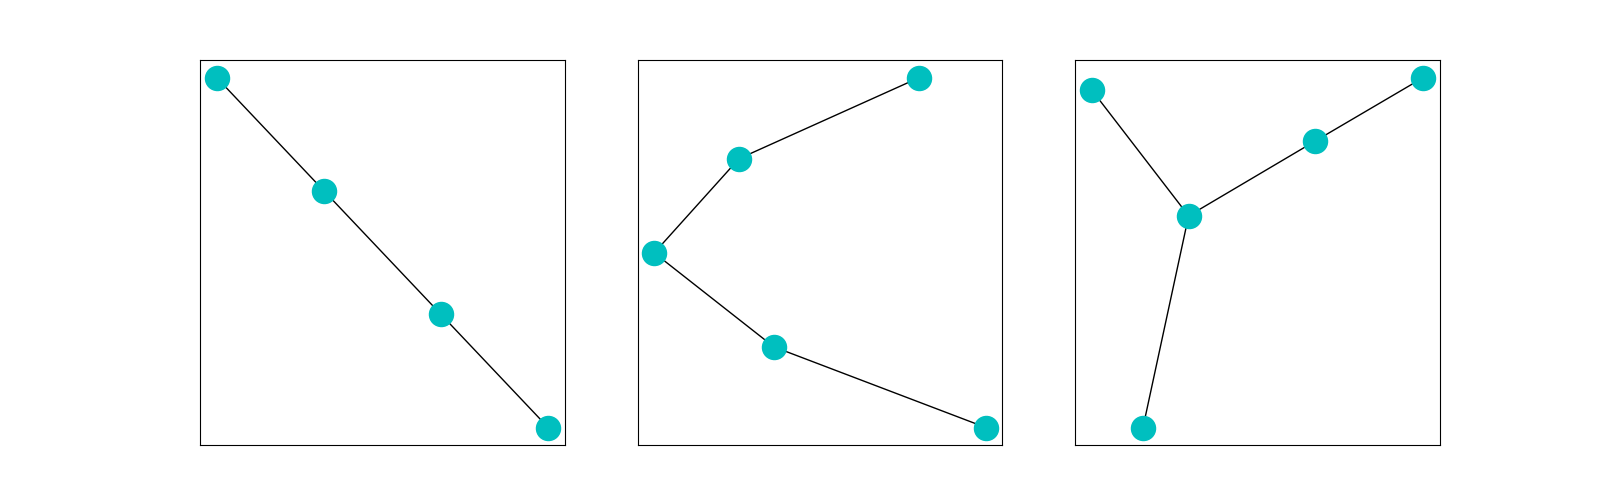
\includegraphics[width=16cm]{Images/H3_evolution.png}
    \centering
    \caption{The possible graphs generated by adding a node to the $H3$ graph 
    and connecting it to an existing node.}
\end{figure}
\FloatBarrier

\begin{table}[h!]
    \centering
        \begin{tabular}{||c c c c||} 
            \hline
            Motif Count & Original Motif & Event 1 & Event 2\\ [0.5ex] 
            \hline\hline
            H3 & 1 & 2 & 2\\ 
            \hline
            H4 & 0 & 0 & 1\\
            \hline
        \end{tabular}
        \caption{The rows denote counts of isomorphisms that can be found in either 
        motif. The $H3$, a four walk, can be found twice in the modified $H3$ in event one
        by starting the walk at either end. In the graph produced again we can only find
        two $H3$'s.}
        \label{table:1}
\end{table}

\section{H4}
The $H4$ motif is one of the motifs that are of primary interest given that for any star $S_k$
with $k \geq 3$ we will find ${k \choose 3}$ appearances of the motif. For large
clusters of $H4$ motifs the $H4$ motif count will grow very rapidly in time. Adding a single node and connecting it produces $k$ new $H4$ appearances in $S_k$. The probability
for an event one on the single motif is $0.5$, and for the event two $0.5$. However, a significant
difference in the occurrence of event ones over event twos will encourage more event ones in the future. 

\begin{figure}[!ht]
    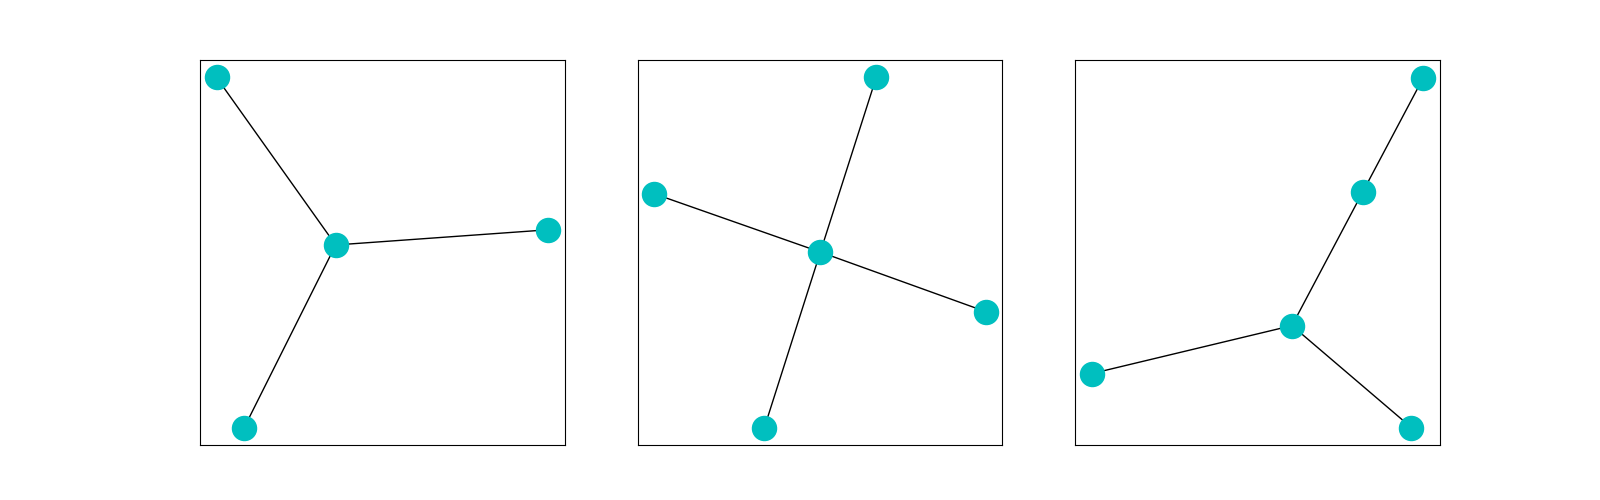
\includegraphics[width=14cm]{Images/H4_evolution.png}
    \centering
    \caption{The possible graphs generated by adding a node to the $H4$ graph 
    and connecting it to an existing node.}
    \label{fig:H4T2}
\end{figure}

\begin{table}[h!]
    \centering
    \begin{tabular}{||c c c c||} 
    \hline
    Motif Count & Original Motif & Event 1 & Event 2\\ [0.5ex] 
    \hline\hline
    H3 & 0 & 0 & 2\\ 
    \hline
    H4 & 1 & 4 & 1\\
    \hline
    H5 & 0 & 0 & 0\\
    \hline
   \end{tabular}
   \caption{Motif Counts of the $H4$ motif and the possible 
   motifs given a $T2$ event.}
    \label{table:2}
\end{table}


\FloatBarrier


\section{H5}
H5's are of interest due to the relationship they carry to the $H4$ motif and the 
$H7$ and $H8$ motifs. The $C_3$ isomorphism in the motif means we find two appearances
$H5$ in the $H7$ and $H8$ motifs. We 
 see the $H4$ is isomorphic to an induced subgraph of the $H5$.The probabilities, given by 
 a preferential attachment mechanism, of the events
  in figure ~\ref{fig:H5T2} event one, $p=0.375$, for event two, $p=0.125$, and event three, $p=0.5$. The last event
only has the highest probability due to symmetry.

\begin{figure}[!ht]
    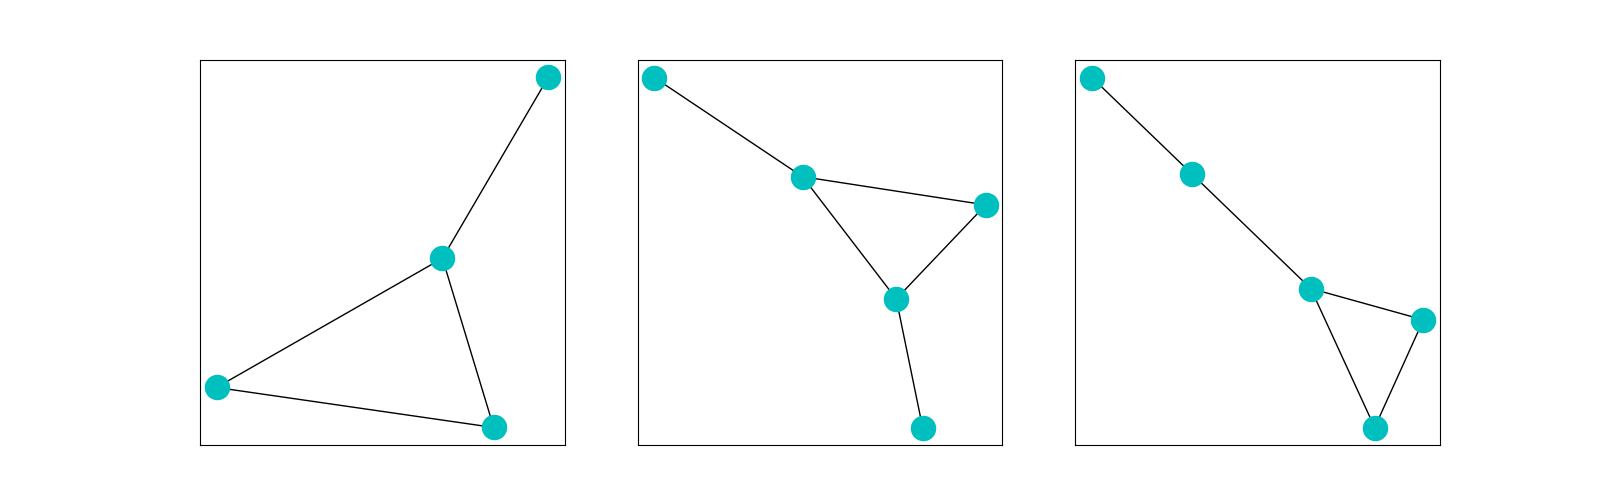
\includegraphics[width=12cm]{Images/H5_evolution.png}
    \centering
    \caption{The possible graphs generated by adding a node to the $H5$ graph 
    and connecting it to an existing node}
    \label{fig:H5T2}
\end{figure}
\FloatBarrier

\begin{table}
    \centering
    \begin{tabular}{||c c c c c||} 
    \hline
    Motif Count & Original Motif & Event 1 & Event 2 & Event 3\\ [0.5ex] 
    \hline\hline
    H3 & 2 & 4 & 4 & 5\\ 
    \hline
    H4 & 1 & 4 & 1 & 2\\
    \hline
    H5 & 1 & 2 & 1 & 2\\
    \hline
    H6 & 0 & 0 & 0 & 0 \\
    \hline
    H7 & 0 & 1 & 0 & 0 \\
    \hline
    H8 & 0 & 0 & 0 & 1\\
    \hline
    H9 & 0 & 0 & 1 & 0\\
    \hline
   \end{tabular}
   \caption{Motif counts of the possible $T2$ events on the $H5$ motif.}
    \label{table:3}
\end{table}


\section{H6}
The $H6$ motif is formed starting with an $H4$ and adding two edges between the three outer nodes. It is 
almost a complete four-node graph. 
The $H6$ motif count is not relatively high when compared to other motifs in the Thij
model because it would require exact $T3$ events to generate them. Moreover, this
$T3$ event has to occur between what are likely non-root nodes. However, in the preferential attachment model for $m>2$
it is more likely to see many $H6$ appearances because of the manner in which 
the preferential attachment model adds multiple edges from a single new node.

\begin{figure}[!ht]
    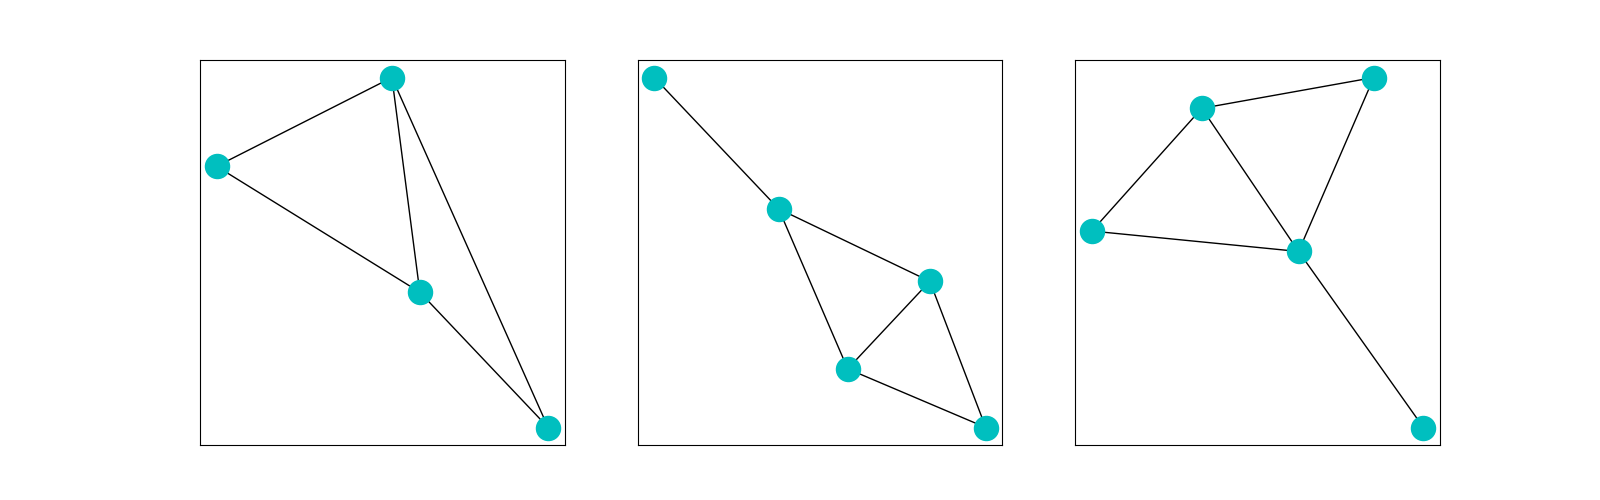
\includegraphics[width=14cm]{Images/H6_evolution.png}
    \centering
    \caption{The possible graphs generated by adding a node to the $H6$ graph 
    and connecting it to an existing node}
\end{figure}
\FloatBarrier

\begin{table}
    \centering
    \begin{tabular}{||c c c c||} 
    \hline
    Motif Count & Original Motif & Event 1 & Event 2\\ [0.5ex] 
    \hline\hline
    H3 & 6 & 10 & 10\\ 
    \hline
    H4 & 2 & 3 & 5\\
    \hline
    H5 & 4 & 5 & 6\\
    \hline
    H6 & 1 & 1 & 1\\
    \hline
    H7 & 0 & 0 & 2\\
    \hline
    H8 & 0 & 2 & 2\\
    \hline
    H9 & 0 & 1 & 1\\
    \hline
    H10 & 0 & 2 & 0\\
    \hline
   \end{tabular}
   \caption{Motif counts for variations of the $T2$ event on the $H6$ motif.}
    \label{table:4}
\end{table}

\section{H7}
$H7$ motifs feature prominently given certain parameters in the Thij model. This is another consequence
of $S_k$ induced subgraphs in the networks. Connecting any two of the outer edges of $S_k$
will generate ${k-2 \choose 2}$ $H7$ motifs. If we generalize it and assume a network has
formed with nodes attached across to all three vertices of a $C_3$ the $H7$ count is
the sum of ${d_i-2 \choose 2}$ for $i=1,2,3$. Adding a node to any one of those vertices, assuming 
$d_i\geq 4$, will generate $d_i-2$ new $H7$ appearances.

\begin{figure}[!ht]
    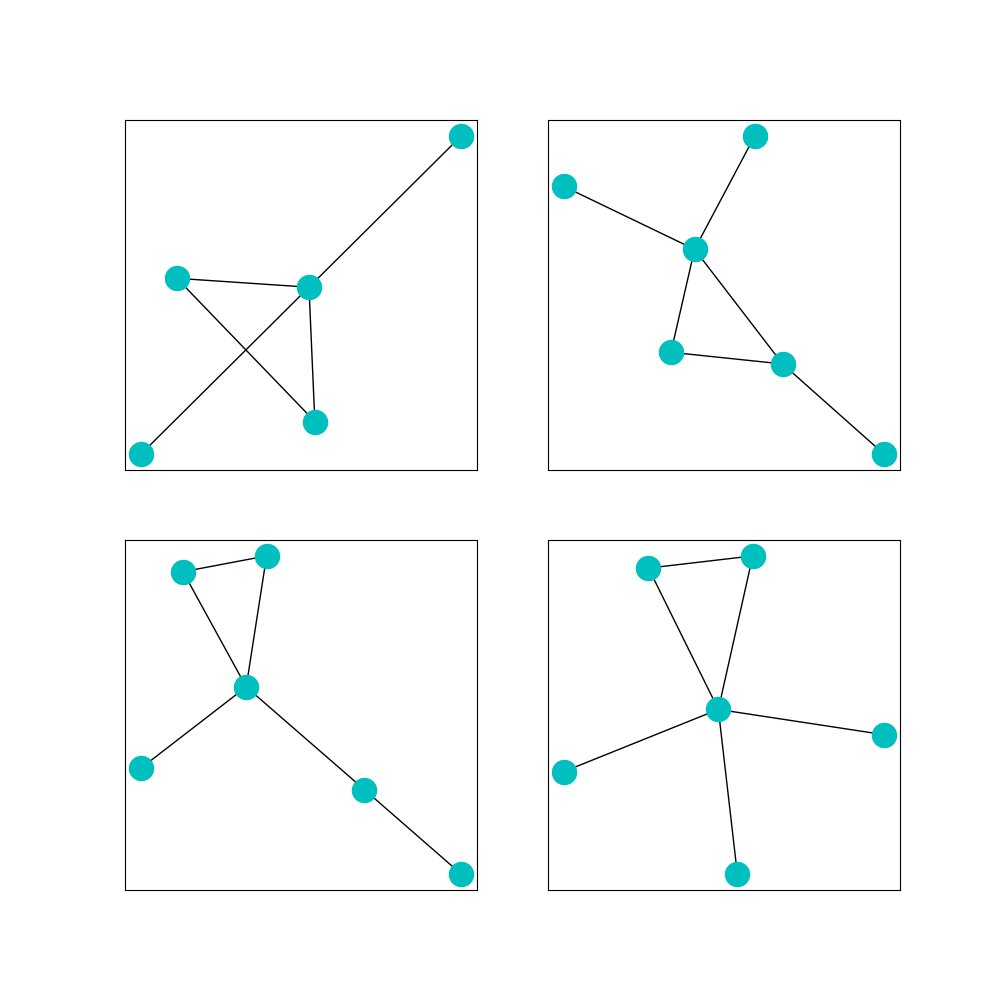
\includegraphics[width=12cm]{Images/H7_evolution.png}
    \centering
    \caption{The possibly graphs generated by adding a node to the $H7$ graph 
    and connecting it to an existing node}
\end{figure}
\FloatBarrier

\begin{table}
    \centering
    \begin{tabular}{||c c c c c||} 
    \hline
    Motif Count & Original Motif & Event 1 & Event 2 & Event 3 \\ [0.5ex] 
    \hline\hline
    H3 & 4 & 8 & 7 & 6\\ 
    \hline
    H4 & 4 & 5 & 4 & 10\\
    \hline
    H5 & 2 & 3 & 2 & 3\\
    \hline
    H6 & 0 & 0 & 0 & 0\\
    \hline
    H7 & 1 & 1 & 1 & 3\\
    \hline
    H8 & 0 & 2 & 0 & 0\\
    \hline
    H9 & 0 & 0 & 0 & 0\\
    \hline
    H10 & 0 & 0 & 1 & 0\\
    \hline
   \end{tabular}
   \caption{Motif counts of the $H7$ motif and the possible additions of $T2$ event nodes.}
   \label{table:5}
\end{table}

\section{H8}
The $H8$ motif is another we expect to appear fairly often. The $H8$
is two $H4$'s sharing an edge and a node. We can also characterize
it as $C_3$ with two nodes attached to distinct vertices on the $C_3$. For the 
$H8$ it is relatively easy to characterize growth as nodes connect
to the vertices of the $C_3$. Given a $C_3$ with at-least one node attached
to each vertex we have $(d_i-2)(d_j-2)(d_k-2)$ $H8's$. The number of new 
$H8$'s by connecting a node to vertex $v_i$ is given by $(d_j-2)(d_k-2)$.

\begin{figure}[!ht]
    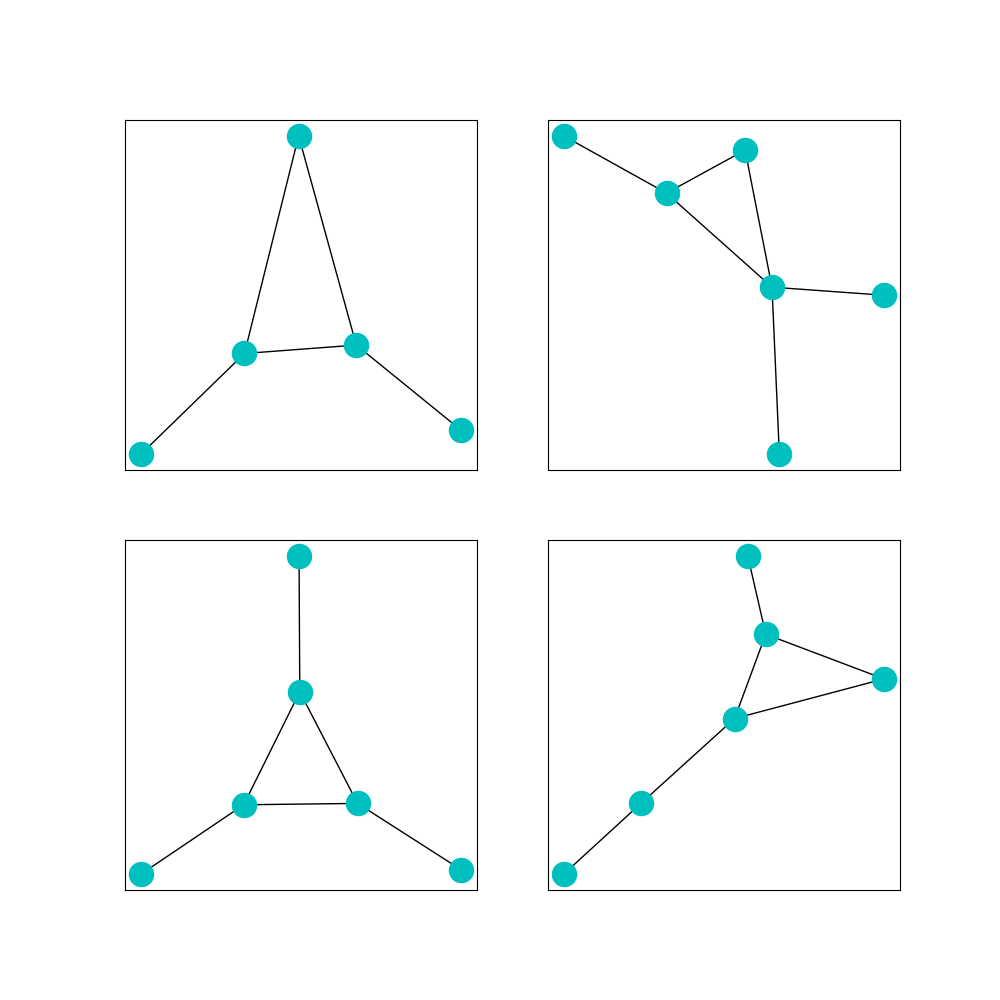
\includegraphics[width=12cm]{Images/H8_evolution.png}
    \centering
    \caption{The possible graphs generated by adding a node to the $H8$ graph 
    and connecting it to an existing node}
\end{figure}

\FloatBarrier
\begin{table}
    \centering
    \begin{tabular}{||c c c c c||} 
    \hline
    Motif Count & Original Motif & Event 1 & Event 2 & Event 3 \\ [0.5ex] 
    \hline\hline
    H3 & 5 & 8 & 9 & 7\\ 
    \hline
    H4 & 2 & 5 & 3 & 2 \\
    \hline
    H5 & 2 & 3 & 3 & 2 \\
    \hline
    H6 & 0 & 0 & 0 & 0 \\
    \hline
    H7 & 0 & 1 & 0 & 0 \\
    \hline
    H8 & 1 & 2 & 3 & 1\\
    \hline
    H9 & 0 & 0 & 0 & 0\\
    \hline
    H10 & 0 & 0 & 0 & 1\\
    \hline
   \end{tabular}
   \caption{Motif counts graphs formed by possible $T2$ events on the $H8$ motif.}
   \label{table:6}
\end{table}

\section{H9}
The $H9$ motifs do not form around stars in the same way we might expect $H7$'s and $H8$'s to do so.
 The $H9$ motif could develop in a way similar to the $H5$. This is because the $H9$ has an induced subgraph
 isomorphic to the $C4$. The $H9$ is produced by attaching a node to any one of those vertices in the induced
 subgraph. Given a $C_4$ and attachment
 of new nodes to any of its four vertices, the count of $H9$'s is simply the sum of the degrees of each
 vertex minus 2. The growth is additive, not combinatorial in the manner of $H7$'s or $H8$'s.

\begin{figure}[!ht]
    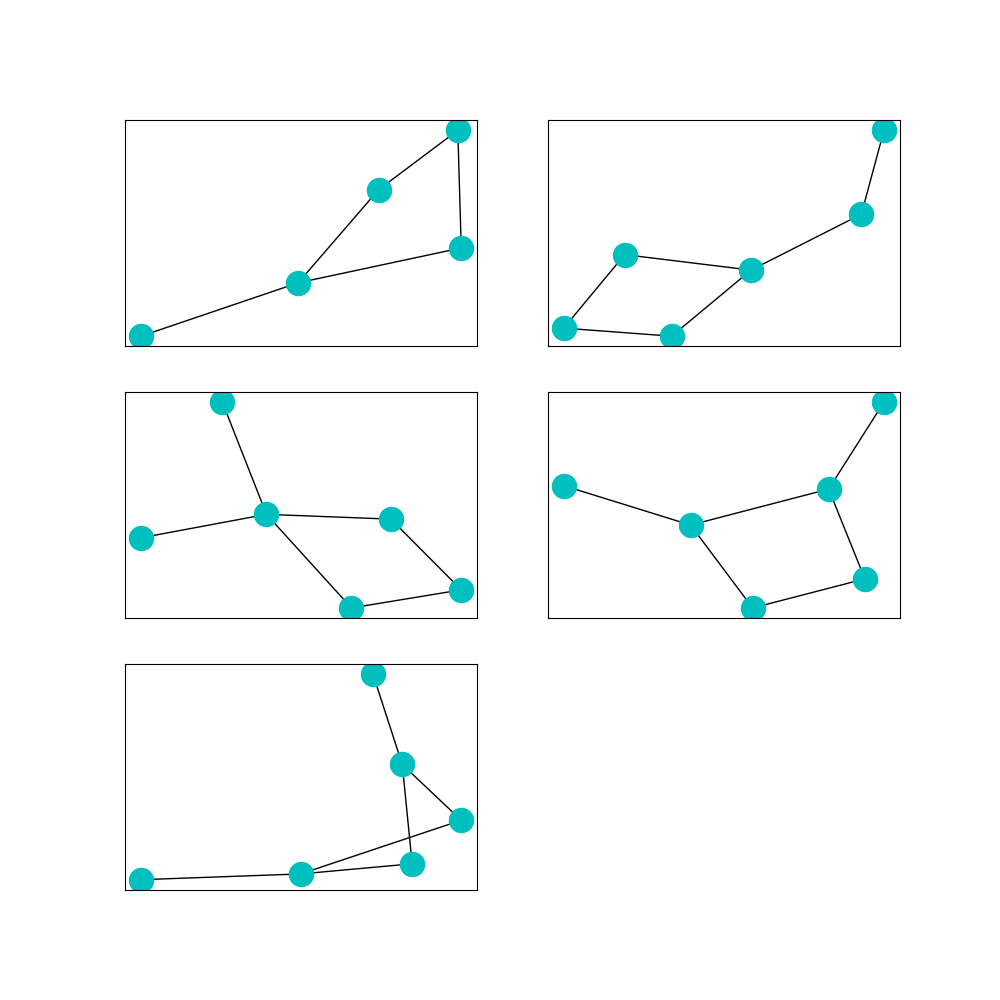
\includegraphics[width=12cm]{Images/H9_evolution.png}
    \centering
    \caption{The possible graphs generated by adding a node to the $H9$ graph 
    and connecting it to an existing node}
\end{figure}

\begin{table}
    \centering
    \begin{tabular}{||c c c c c c ||} 
    \hline
    Motif Count & Original Motif & Event 1 & Event 2 & Event 3  & Event 4\\ [0.5ex] 
    \hline\hline
    H3 & 6 & 8 & 8 & 9 & 8\\ 
    \hline
    H4 & 1 & 1 & 4 & 2 & 2 \\
    \hline
    H5 & 0 & 0 & 0 & 0 & 0\\
    \hline
    H6 & 0 & 0 & 0 & 0 & 0\\
    \hline
    H7 & 0 & 0 & 0 & 0 & 0\\
    \hline
    H8 & 0 & 0 & 0 & 0& 0\\
    \hline
    H9 & 1 & 1 & 2 & 2 &2\\
    \hline
   \end{tabular}
   \caption{Motif counts graphs formed by possible $T2$ events on the $H9$ motif.}
   \label{table:7}
\end{table}

\section{H10}
The $H10$ is the $H9$ with an extra vertex and an edge between that vertex to the 
single vertex of degree one in the $H9$. Many $H10$'s could be generated from a single $H9$ if vertices
attach to the single vertex of degree one in the $H9$ motif. A star graph would form
with that vertex at the center. The growth for the $H10$ in the preferential mechanism with $k=1$ is additive.
For $k>1$, it is possible clusters of triangles to see the $H10$ motif count to grow faster than what one would
see, adding a single node and edge at each time step. 

\begin{figure}[!ht]
    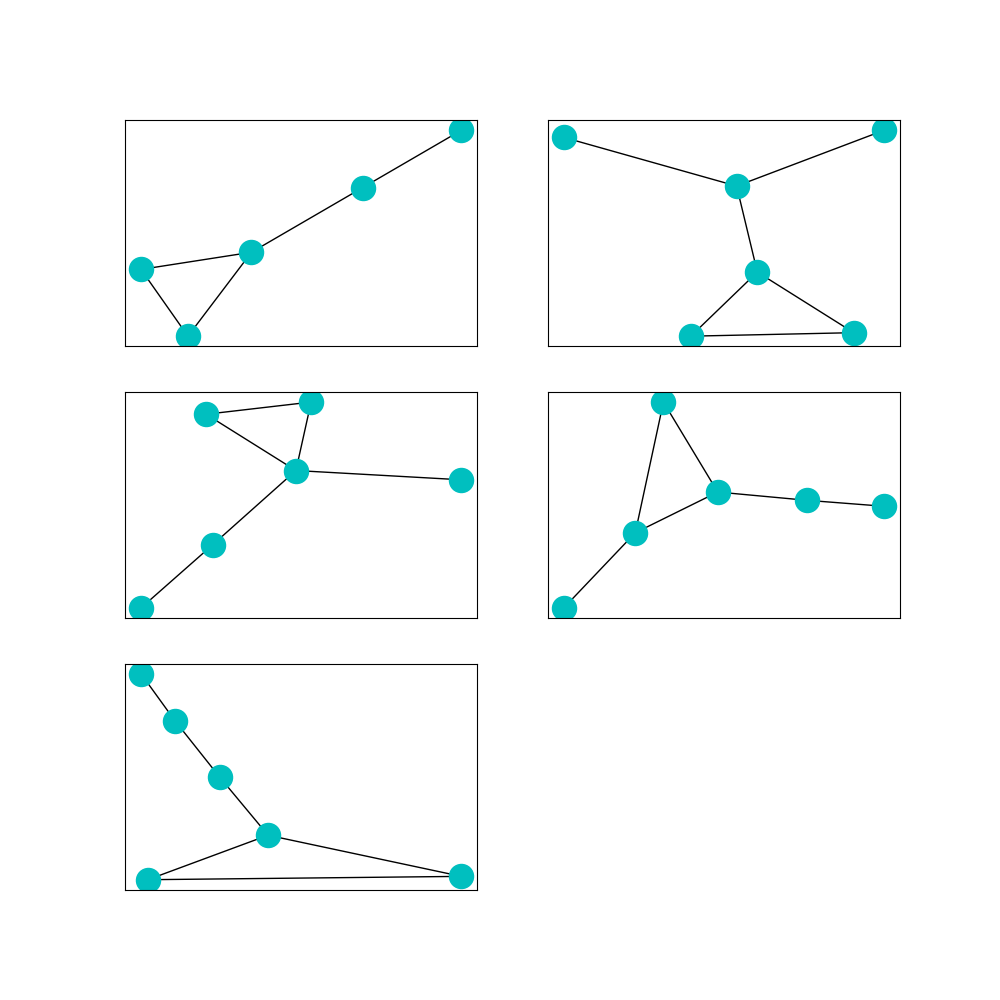
\includegraphics[width=12cm]{Images/H10_evolution.png}
    \centering
    \caption{The possible graphs generated by adding a node to the $H10$ graph 
    and attaching it to an existing node.}
\end{figure}

\begin{table}
    \centering
    \begin{tabular}{||c c c c c c ||} 
    \hline
    Motif Count & Original Motif & Event 1 & Event 2 & Event 3  & Event 4 \\ [0.5ex] 
    \hline\hline
    H3 & 4 & 6 & 7 & 7  & 5\\
    \hline
    H4 & 1 & 2 & 4 & 2  & 1\\
    \hline
    H5 & 1 & 1 & 2 & 2 & 1\\
    \hline
    H6 & 0 & 0 & 0 & 0  & 5\\
    \hline
    H7 & 0 & 0 & 1 & 0 & 0 \\
    \hline
    H8 & 0 & 0 & 0 & 1 & 0 \\
    \hline
    H9 & 0 & 0 & 0 & 0  & 0 \\
    \hline
    H10 & 1 & 2 & 1 & 1 & 1 \\
    \hline
   \end{tabular}
   \caption{Motifs counts of the possible $T2$ event on the $H10$ motif.}
   \label{table:8}
\end{table}

\FloatBarrier

\section{H11}
The $H11$ motif, shaped like a bow-tie, is formed by two three-walks that share a common
vertex. This motif does need $k \geq 2$ in the Barabási–Albert Model or a 
 a $T3$ event to form an edge between two existing nodes. The $H11$ motif does not appear 
 commonly without those necessary criteria.

\begin{figure}[!ht]
    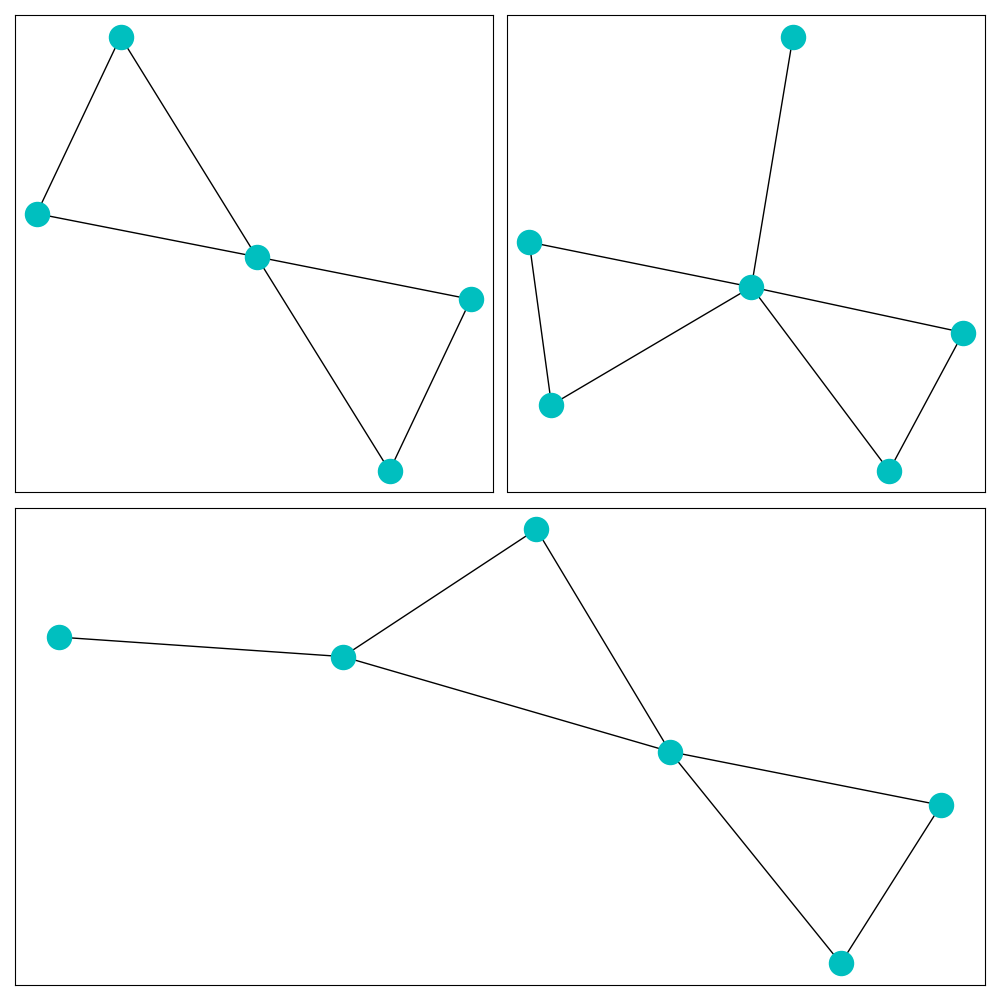
\includegraphics[width=8cm]{Images/H11_evolution.png}
    \centering
    \caption{The possibly graphs generated by adding a node to the $H11$ graph 
    and connecting it to an existing node.}
\end{figure}

\begin{table}
    \centering
    \begin{tabular}{||c c c c||} 
    \hline
    Motif Count & Original Motif & Event 1 & Event 2 \\ [0.5ex] 
    \hline\hline
    H3 & 8 & 12 & 12 \\ 
    \hline
    H4 & 4 & 5 & 10  \\
    \hline
    H5 & 0 & 5 & 6  \\
    \hline
    H6 & 0 & 0 & 0  \\
    \hline
    H7 & 2 & 2 & 6 \\
    \hline
    H8 & 0 & 2 & 0 \\
    \hline
    H9 & 0 & 0 & 0 \\
    \hline
    H10 & 4 & 5 & 4 \\
    \hline
    H11 & 1 & 1 & 1\\
    \hline
   \end{tabular}
   \caption{Motif counts of the graphs generated by possible $T2$ events on the $H11$ motif.}
   \label{table:9}
\end{table}

\FloatBarrier

\section{H12}
$H12$, shaped like a house, contains five nodes, six edges, with an induced subgraph isomorphic to $C_4$
and a single vertex attached to two vertices they connected. The $H12$, like other
motifs, contains an induced subgraph isomorphic to $C_4$ is not a priori expected to have a relatively large count
given the preferential attachment mechanism. 

\begin{figure}[!ht]
    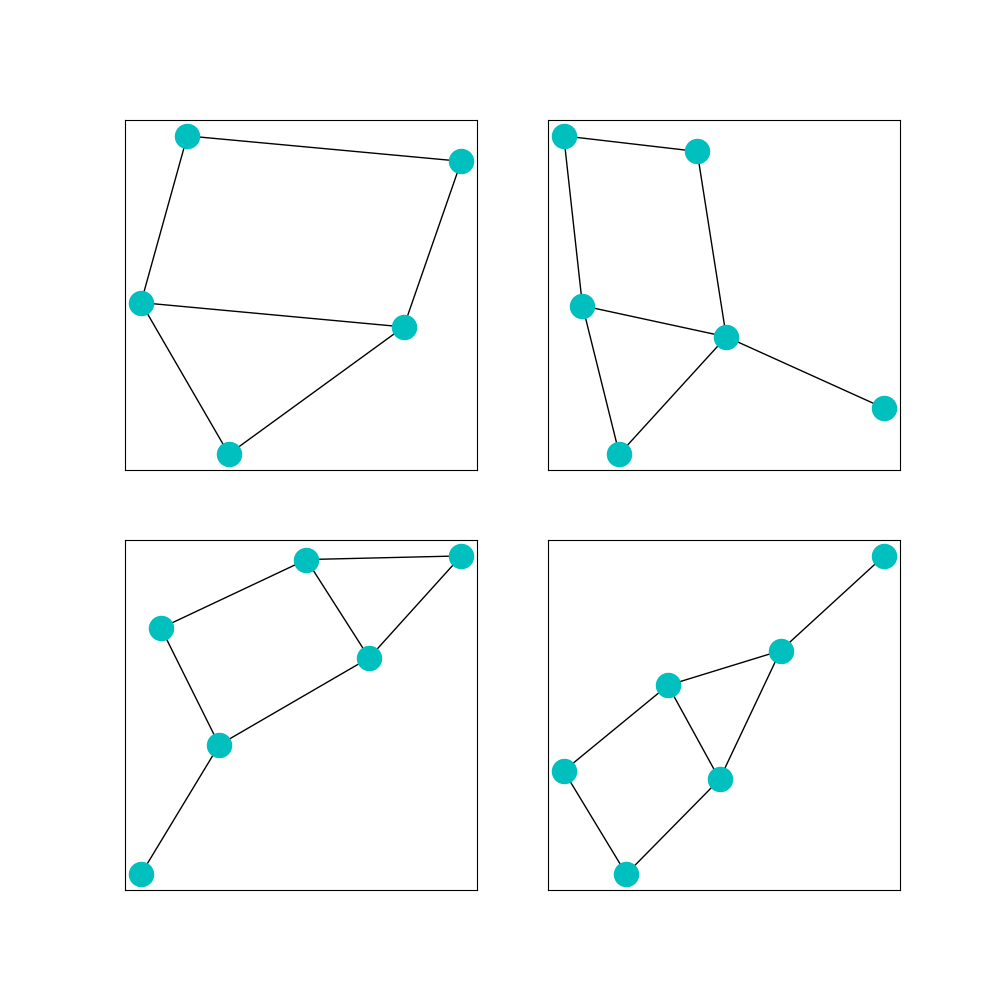
\includegraphics[width=12cm]{Images/H12_evolution.png}
    \centering
    \caption{The possibly graphs generated by adding a node to the $H12$ graph 
    and connecting it to an existing node.}
\end{figure}

\begin{table}
    \centering
    \begin{tabular}{||c c c c c||} 
    \hline
    Motif Count & Original Motif & Event 1 & Event 2 & Event 3 \\ [0.5ex] 
    \hline\hline
    H3 & 10 & 14 & 13 & 14\\ 
    \hline
    H4 & 2 & 5 & 3 & 3 \\
    \hline
    H5 & 2 & 3 & 2 & 3 \\
    \hline
    H6 & 0 & 0 & 0 & 0 \\
    \hline
    H7 & 0 & 1 & 0 & 0 \\
    \hline
    H8 & 1 & 2 & 1 & 3\\
    \hline
    H9 & 2 & 3 & 3 & 2 \\
    \hline
    H10 & 2 & 2 & 3 & 2 \\
    \hline
    H11 & 0 & 0 & 0 & 0 \\
    \hline
    H12 & 1 & 1 & 1 & 1\\
    \hline
   \end{tabular}
   \caption{Variations of the $T2$ event on the $H12$ motif}
   \label{table:10}
\end{table}


\FloatBarrier

\section{H13}
The $H13$ could plausibly form in the $k \geq 2$ case for the 
Barabási–Albert model, but it would require a new node being consistently attached to the
same two nodes repeatedly. If this process of generating new $H13$'s, the increase in the motif counts is additive.
 Thus for the Barabási–Albert model of $0<k<3$, the presence of an $H13$ is sensitive
to the initial graph and its early development when there might still be a 'more uniform' probability
of attachment.

\begin{figure}[!ht]
    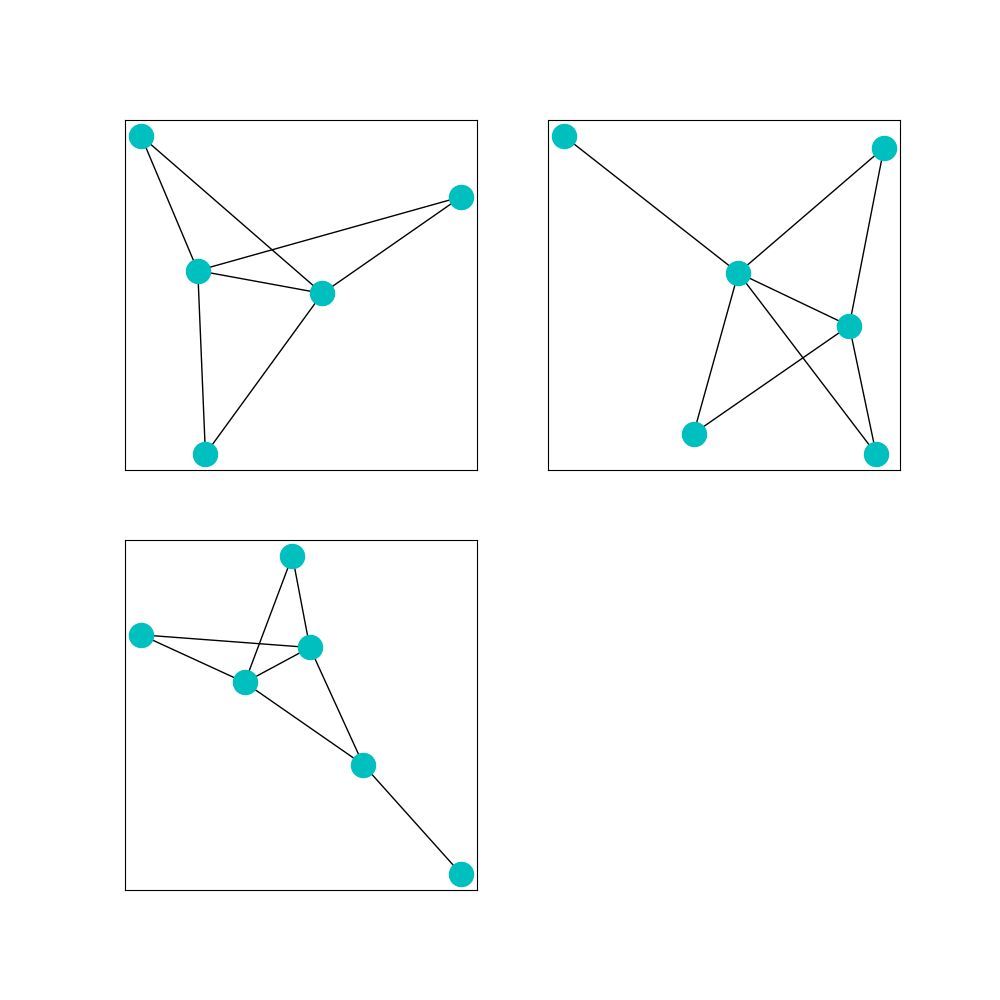
\includegraphics[width=8cm]{Images/H13_evolution.png}
    \centering
    \caption{The H13 graph and possible node attachments up to symmetry.}
\end{figure}

\begin{table}
    \centering
    \begin{tabular}{||c c c c||} 
    \hline
    Motif Count & Original Motif & Event 1 & Event 2 \\ [0.5ex] 
    \hline\hline
    H3 & 18 & 24 & 24\\ 
    \hline
    H4 & 8 & 14 & 9  \\
    \hline
    H5 & 12 & 15 & 13  \\
    \hline
    H6 & 3 & 3 &3  \\
    \hline
    H7 & 6 & 12 & 6 \\
    \hline
    H8 & 6 & 12 & 10\\
    \hline
    H9 & 6 & 9 & 8 \\
    \hline
    H10 & 0 & 0 & 4  \\
    \hline
    H11 & 0 & 0 & 0  \\
    \hline
    H12 & 0 & 0 & 0 \\
    \hline
    H13 & 1 & 1 & 1 \\
    \hline
   \end{tabular}
   \caption{Motif counts of the possible $T2$ events on the $H13$ motif}
   \label{table:11}
\end{table}

\section{Summary of Preferential Attachment and $T2$ Event Motif Evolution}


Motif developement in the Barabási–Albert model is dependent on how the model is initialized and 
the choice of $k$. If we only add $k=1$ edges for every new node
this limits the types of motifs that can appear. There will be no new $H6$'s, $H11$'s,
$H12$'s, or $H13$'s generated. There is no possible way for them to form as there is no
node of degree one in those motifs. Only upon taking $k>1$ could those motif counts change over
 time. Some graphs still are more likely for $k=2$ than others like the $H4$'s, $H7$'s, and $H8$'s.

This analysis also applies to the $T2$ event in the Thij model. The occurrence is similar to
the preferential attachment model with $k=1$ as it is simply the addition of a node which is then
connected to a single existing node. The $T2$ event, unlike the BA model, selects a message tree 
and then uses a superstar attachment mechanism to attach to a node with probability $q=0.9$. Even when the network is relatively
small nodes will still overwhelmingly attach to the root message node. This mechanism is
much more probable to generate $H4$'s as seen above in chapter 3. If the root
message node is the vertex of a $C_3$ then we may see $H7$ and $H8$ counts
rapidly increase over time, correlating with the $H4$ count. 

\chapter{Twitter Model Specific Motif Evolution}

In chapter 3, we specified three possible
events in the Thij model: a new root node, a new node and an attached edge, or a new edge between existing nodes 
($T1$, $T2$, $T3$ respectively). The only event specific to the Thij model are $T1$ and $T3$ events. 
$T1$ events add a new message node, but they don't immediately affect any change in the motif counts.
They could potentially with the right $T3$ event or a series of $T2$ events. The $T3$ event we must consider, because
 a $T3$ event can change the composition of the network in ways $T2$ events cannot. Given that a $T3$ event is
occurring it follows first, the preferential-attachment mechanism for tree selection, then follows superstar 
probability for source node selection, and then finally uniform probability for target node selection.
This makes it difficult
to discuss the associated probabilities of a potential $T3$ event. We may suspect
a root message node within a graph based on its degree, but may not know without prior knowledge
of the data. We can examine how each $T3$ event will affect a given motif graph provided the $T3$
event occurs between nodes in the motif.

\section{H3}
The $H3$ motif only has two possible events. We see either an $H5$ form by connecting
an outer vertex to the opposite inner or the outer two vertices are connected
forming a four-cycle. Future development of this new $H5$ in the context of 
$T3$ events is discussed in section 6.3. 

\begin{figure}[!ht]
    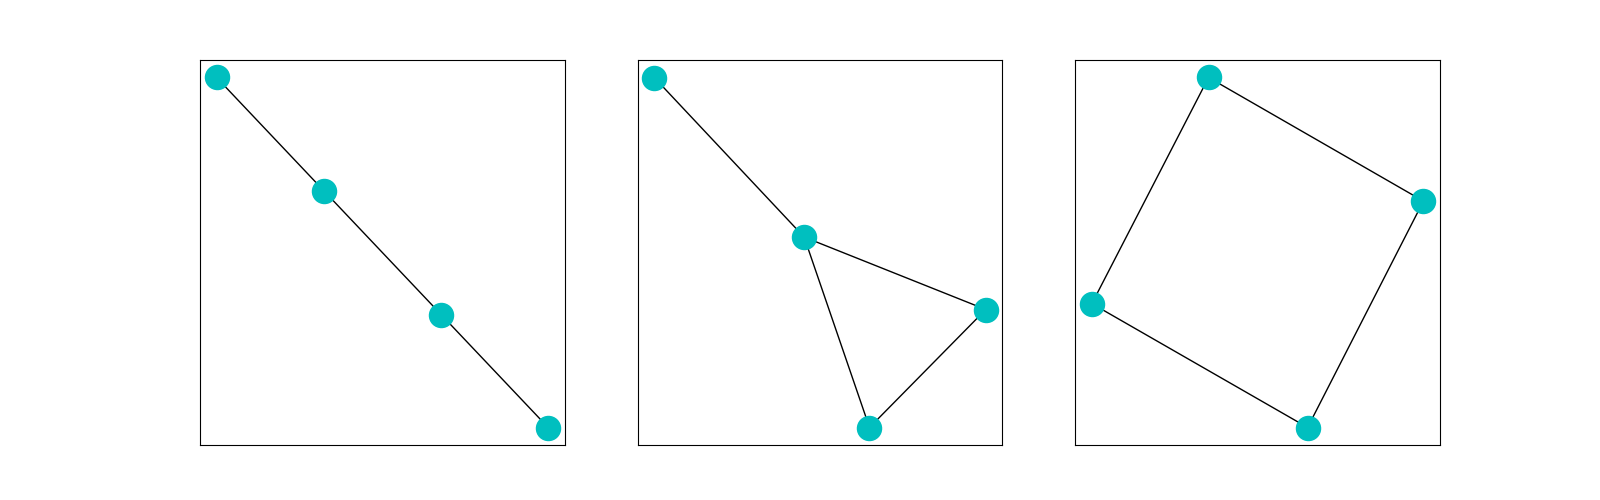
\includegraphics[width=15cm]{Images/H3_T3_evolution.png}
    \centering
    \caption{The possible graphs generated by adding an edge to the $H3$ graph.}
\end{figure}

\begin{table}
    \centering
    \begin{tabular}{||c c c c||} 
    \hline
    Motif Count & Original Motif & Event 1 & Event 2\\ [0.5ex] 
    \hline\hline
    H3 & 1 & 2 & 4\\ 
    \hline
    H4 & 0& 1 & 0  \\
    \hline
    H5 & 0& 1 & 0  \\
    \hline
   \end{tabular}
   \caption{Motif counts of the possible $T3$ events on the $H3$ motif}
   \label{table:12}
\end{table}

\section{H4}
Due to the three symmetry of the $H4$, adding an edge between any two unconnected nodes creates a single $H5$. Therefore given some balance between $T2$ and $T3$ events
we could see correlation between these two motifs.

\begin{figure}[!ht]
    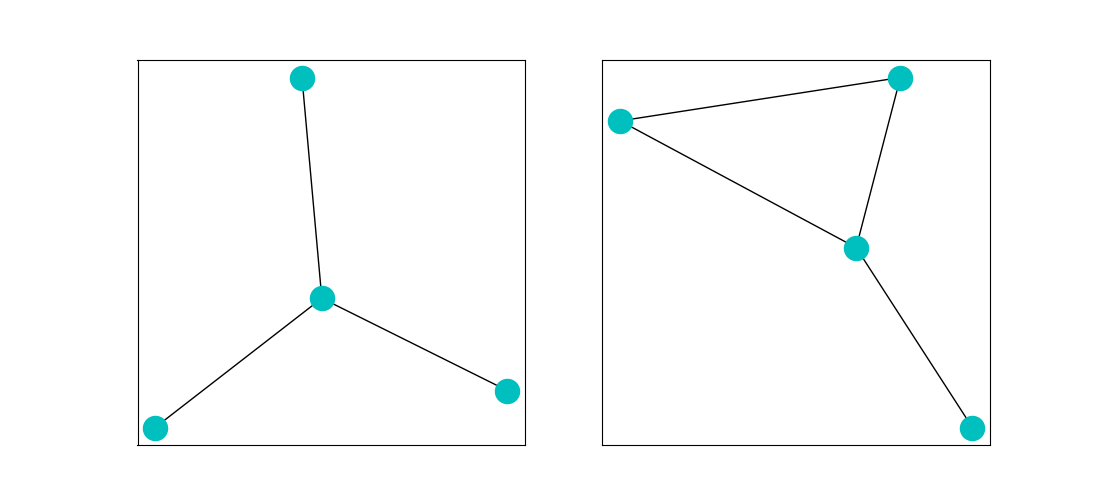
\includegraphics[width=14cm]{Images/H4_T3_evolution.png}
    \centering
    \caption{The possible graphs generated by adding an edge to the $H4$ graph. By connecting the 
    two outer edges we find a $C_4$ and by connecting an outer vertex to an inner vertex we generate a $H5$.}
\end{figure}

\begin{table}
    \centering
    \begin{tabular}{||c c c||} 
    \hline
    Motif Count & Original Motif & Event 1 \\ [0.5ex] 
    \hline
    H3 & 0 & 2 \\ 
    \hline
    H4 & 1 & 1 \\
    \hline
    H5 & 0 & 1 \\
    \hline
   \end{tabular}
   \caption{Motif counts of the $T3$ event on the $H4$ motif}
   \label{table:13}
\end{table}

\section{H5}
The $H5$ motif is symmetric. Connecting any two unconnected vertices of the $H5$ produces an $H6$.
A $H4$ with a $T3$ event creates an $H5$ graph. A $T3$ event occurs again on the same graph and a $H6$
graph is produced.

\begin{figure}[!ht]
    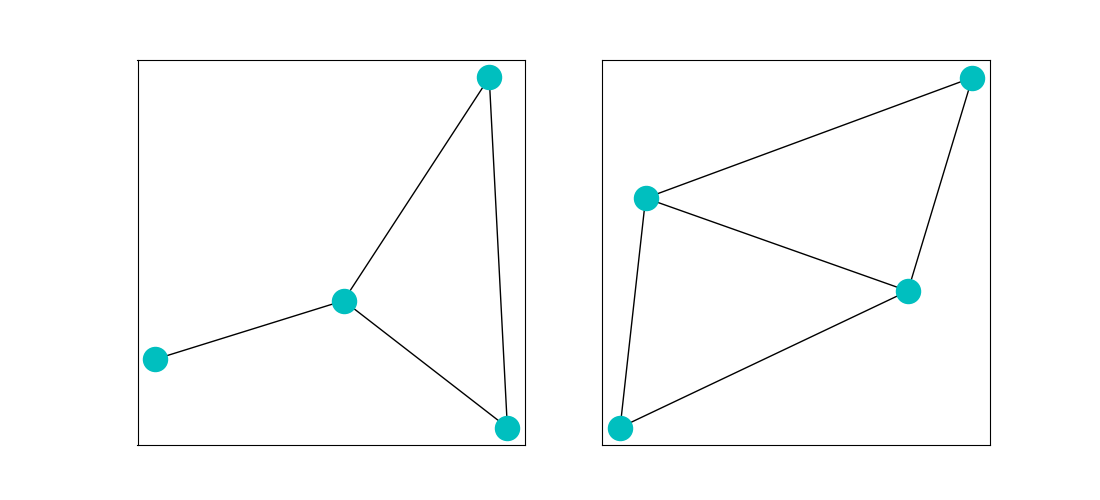
\includegraphics[width=14cm]{Images/H5_T3_evolution.png}
    \centering
    \caption{The possible graphs generated by adding an edge to the $H5$ graph.}
\end{figure}

\begin{table}
    \centering
    \begin{tabular}{||c c c||} 
    \hline
    Motif Count & Original Motif & Event 1 \\ [0.5ex] 
    \hline\hline
    H3 & 2 & 6\\ 
    \hline
    H4 & 1 & 2 \\
    \hline
    H5 & 1 & 4\\
    \hline
    H6 & 0 & 1\\
    \hline
   \end{tabular}
   \caption{Motif counts of the graphs produced by a $T3$ event on the $H5$ motif.}
   \label{table:14}
\end{table}

\section{H6}
Adding an edge to $H6$ generates a complete graph of four nodes. This 
event is unlikely given a large graph, but not impossible. If a vertex
of the $H6$ is a message node then an edge could be added within the $H6$ graph. 
However, an edge added between the $H6$ appearance and the appearance of another 
motif is more likely. 

\begin{figure}[!ht]
    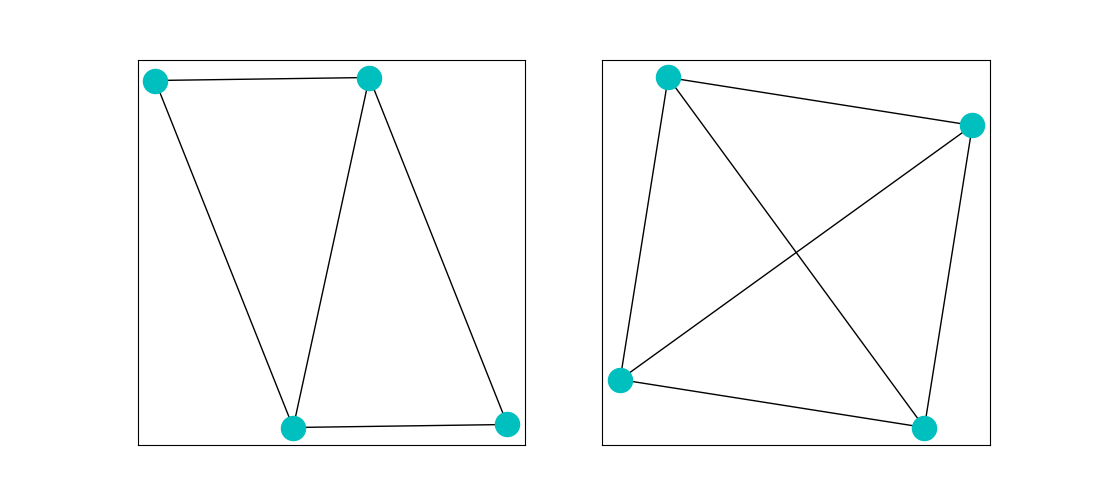
\includegraphics[width=14cm]{Images/H6_T3_evolution.png}
    \centering
    \caption{The possible graphs generated by adding an edge to the $H6$ graph.}
\end{figure}

\begin{table}
    \centering
    \begin{tabular}{||c c c ||} 
    \hline
    Motif Count & Original Motif & Event 1  \\ [0.5ex] 
    \hline\hline
    H3 & 6 & 12 \\ 
    \hline
    H4 & 2 & 4 \\
    \hline
    H5 & 4 & 12 \\
    \hline
    H6 & 1 & 6 \\
    \hline
    \hline
   \end{tabular}
   \caption{Motif counts of graph produced by a $T3$ event on the $H6$ motif.}
\end{table}

\section{H7}
Adding edges, the $H7$ motif gives only two non-isomorphic graphs as 
a consequence of the motif's symmetry. Given an event two in figure ~\ref{fig:H7T3} the graph becomes
an $H11$. Both events do show that one could see a high $H7$ count given enough
clustering around a message node. 
 
\begin{figure}[!ht]
    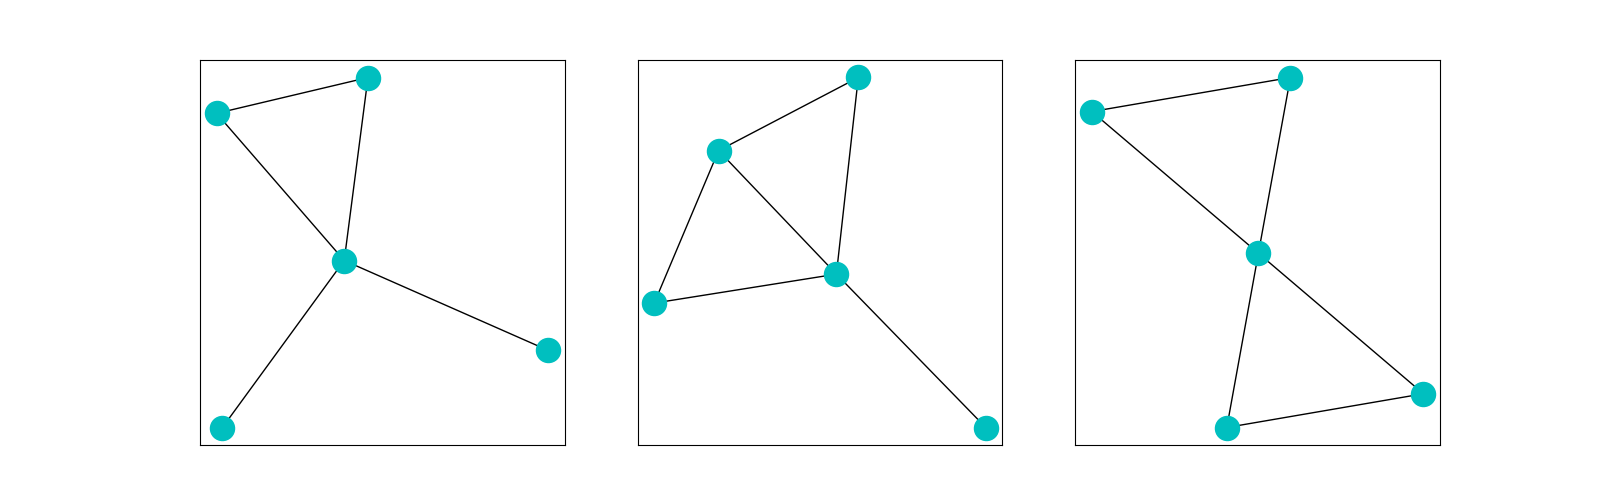
\includegraphics[width=16cm]{Images/H7_T3_evolution.png}
    \centering
    \caption{The possible graphs generated by adding an edge to the $H7$ graph.}
    \label{fig:H7T3}
\end{figure}

\begin{table}
    \centering
    \begin{tabular}{||c c c c||} 
    \hline
    Motif Count & Original Motif & Event 1 & Event 2  \\ [0.5ex] 
    \hline\hline
    H3 & 4 & 10 & 8\\ 
    \hline
    H4 & 4 & 5& 4 \\
    \hline
    H5 & 2 & 6 & 4 \\
    \hline
    H6 & 0 & 1 & 0 \\
    \hline
    H7 & 1 & 2 & 2 \\
    \hline
    H8 & 0 & 2 & 0\\
    \hline
    H9 & 0 & 1 & 0 \\
    \hline
    H10 & 0 & 0 & 4 \\
    \hline
    H11 & 0 & 0 & 1\\
    \hline
   \end{tabular}
   \caption{Motif counts of the two possible graphs produced by the $T3$ event on the $H7$ motif}
   \label{table:16}
\end{table}

\section{H8}
The $H8$ motif here generates three different motifs depending upon the nodes which become connected.
The $H8$ motif if similar to the $H7$ motif as clusters of triangles can contain many $H8$ appearances. 

\begin{figure}[!ht]
    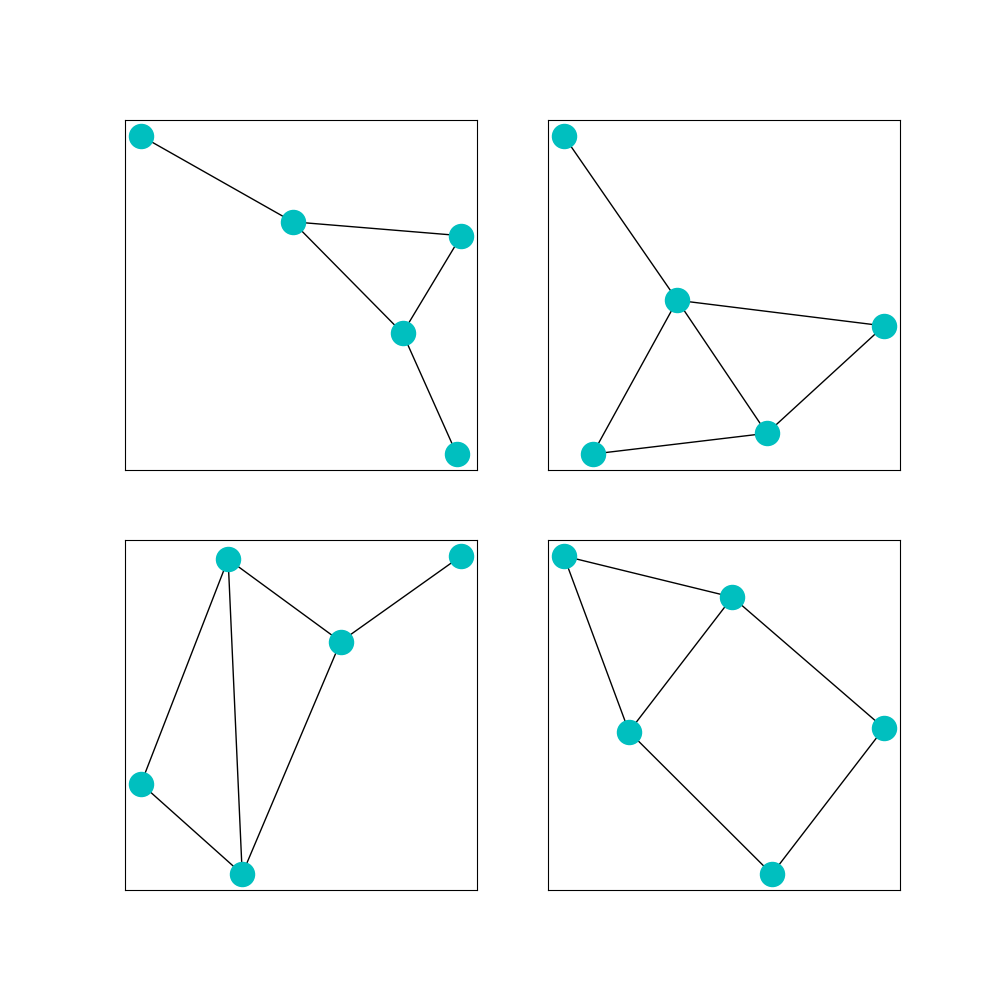
\includegraphics[width=12cm]{Images/H8_T3_evolution.png}
    \centering
    \caption{The possible graphs generated by adding an edge to the $H8$ graph.}
\end{figure}

\begin{table}
    \centering
    \begin{tabular}{||c c c c c||} 
    \hline
    Motif Count & Original Motif & Event 1 & Event 2 & Event 3 \\ [0.5ex] 
    \hline\hline
    H3 & 5 & 10 & 10 & 10\\ 
    \hline
    H4 & 2 & 5 & 3 & 2 \\
    \hline
    H5 & 2 & 6 & 5 & 2 \\
    \hline
    H6 & 0 & 1 & 1 & 0 \\
    \hline
    H7 & 0 & 2 & 0 & 0 \\
    \hline
    H8 & 1 & 2 & 2 & 1\\
    \hline
    H9 & 0 & 1 & 1 & 2\\
    \hline
    H10  & 0 & 0 & 2& 2 \\
    \hline
    H11  & 0 & 0 & 1& 0 \\
    \hline
    H12  & 0 & 0 & 0& 0 \\
    \hline
   \end{tabular}
   \caption{Motif counts of the possible $T3$ event on the $H8$ motif}
   \label{table:17}
\end{table}

\section{H9}
An $H9$ motif with an edge added anywhere does not produce a combinatorial jump in counts as
 other motifs might. The $H9$ had an induced subgraph, isomorphic to the $C_4$ which
 means the graph requires more events or the right intialization to generate itself. Given
 a high $T3$ probability there relatively high $H9$ counts as seen in figures ~\ref{fig:pthij0202}
and ~\ref{fig:pthij0802}.

\begin{figure}
    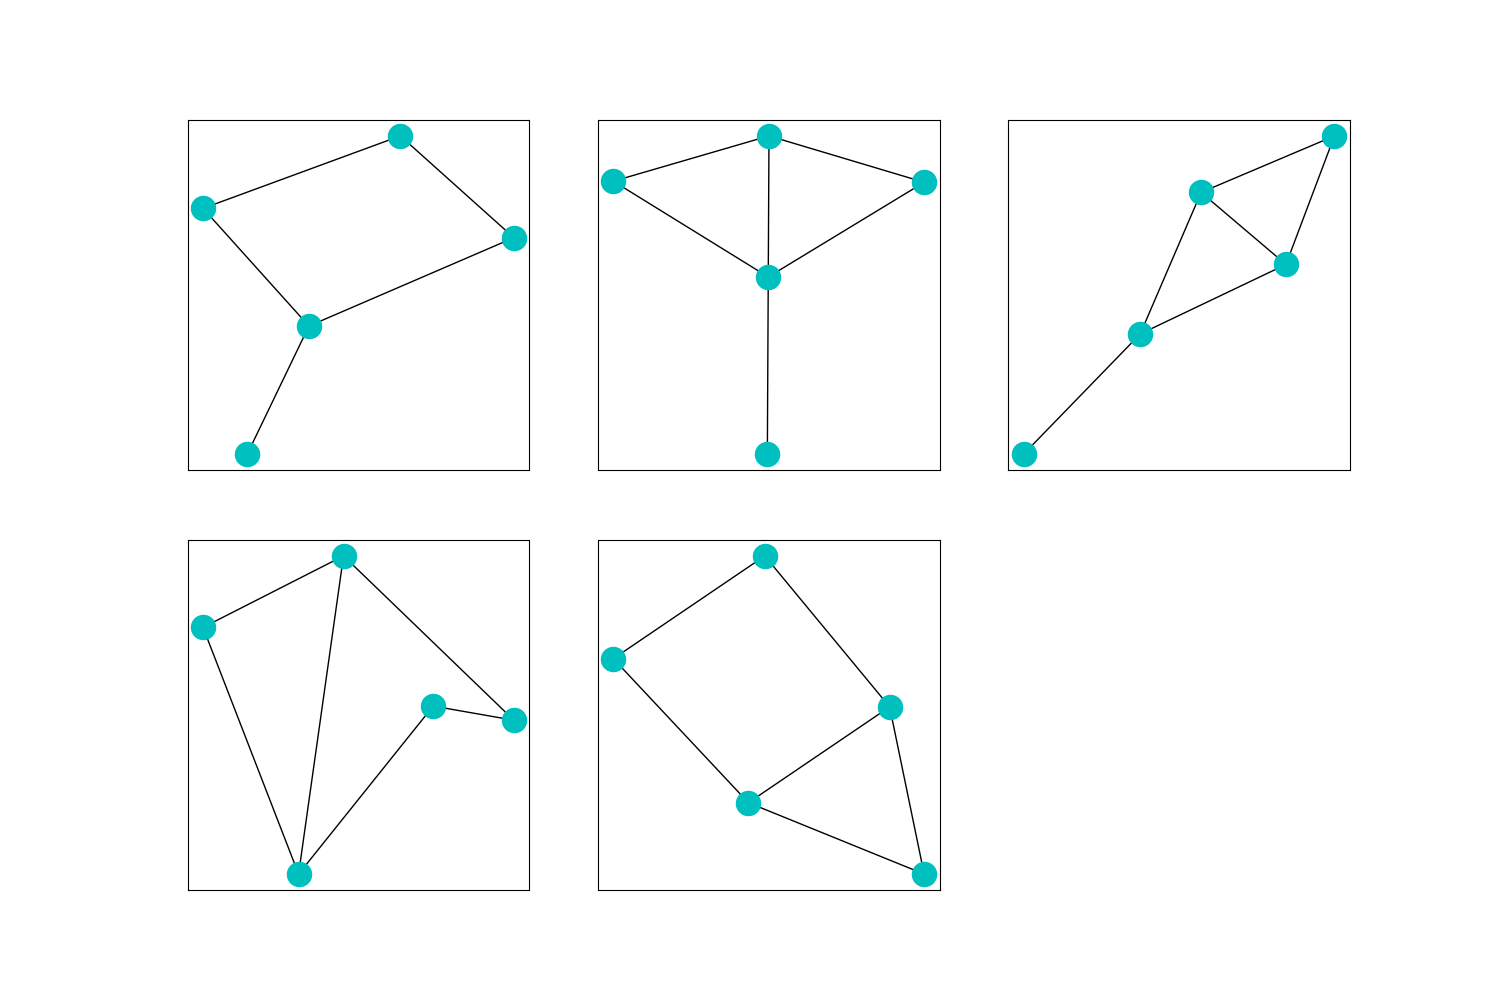
\includegraphics[width=14cm]{Images/H9_T3_evolution.png}
    \centering
    \caption{The possible graphs generated by adding an edge to the $H9$ graph.}
\end{figure}

\begin{table}
    \centering
    \begin{tabular}{||c c c c c c||} 
    \hline
    Motif Count & Original Motif & Event 1 & Event 2 & Event 3 & Event 4 \\ [0.5ex] 
    \hline\hline
    H3 & 6 & 10 & 10 & 10 & 10\\ 
    \hline
    H4 & 1 & 5 & 3 & 2 & 2 \\
    \hline
    H5 & 0 & 6 & 5 & 2 & 2 \\
    \hline
    H6 & 0 & 1 & 1 & 0 & 0 \\
    \hline
    H7 & 1 & 2 & 1 & 0 & 0 \\
    \hline
    H8 & 0 & 2 & 2 & 1 & 1\\
    \hline
    H9 & 1 & 1 & 2 & 2 & 2\\
    \hline
    H10 & 0 & 0 & 2 & 2 & 2\\
    \hline
    H11 & 0 & 0 & 0 & 0 & 0\\
    \hline
    H12 & 0 & 0 & 0 & 1 & 1\\
    \hline
   \end{tabular}
   \caption{Motif counts of the possible $T3$ event on the $H9$ motif}
   \label{table:18}
\end{table}

\section{H10}
The $H10$ motif features in those Thij models with $p<0.5$ line in figures ~\ref{fig:pthij0202} and
~\ref{fig:pthij0808}, given
that there is enough likelihood a $T3$ event occurs acting on an $H9$. For events two, three, and four below
in Figure~\ref{fig:H10T3}, attaching a node to the $H10$ motif produces a handful more of $H10$'s.


\begin{figure}
    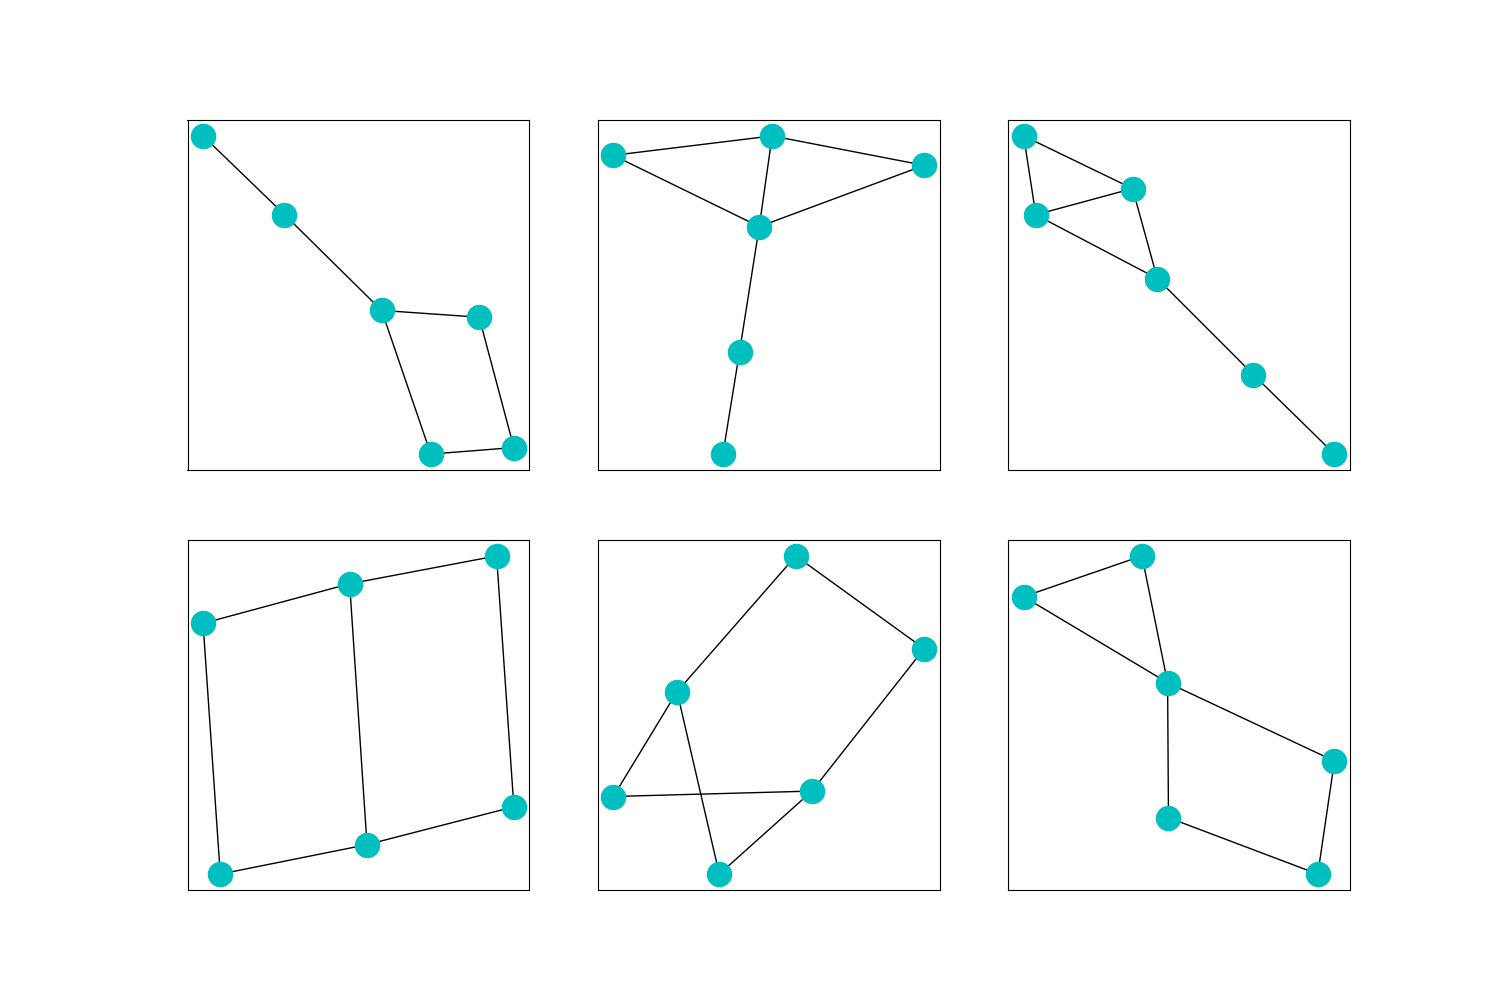
\includegraphics[width=12cm]{Images/H10_T3_evolution.png}
    \centering
    \caption{The possible graphs generated by adding an edge to the $H10$ graph.}
    \label{fig:H10T3}
\end{figure}

\begin{table}
    \centering
    \begin{tabular}{||c c c c c||} 
    \hline
    Motif Count & Original Motif & Event 1 & Event 2 & Event 3 \\ [0.5ex] 
    \hline\hline
    H3 & 4 & 10 & 8 & 10 \\ 
    \hline
    H4 & 1 & 2 & 4 & 3 \\
    \hline
    H5 & 1 & 2 & 4 & 5\\
    \hline
    H6 & 0 & 0 & 0 & 1 \\
    \hline
    H7 & 0 & 0 & 2 & 0 \\
    \hline
    H8 & 0 & 1 & 0 & 2\\
    \hline
    H9 & 0 & 2 & 0 & 1\\
    \hline
    H10 & 1 & 2 & 4 & 2\\
    \hline
    H11 & 0 & 0 & 1 & 0\\
    \hline
    H12 & 0 & 1 & 0 & 0\\
    \hline
   \end{tabular}
   \caption{Motif counts of the graphs given by a $T3$ event on the $H10$ motif}
   \label{table:19}
\end{table}

\section{H11}
$H11$'s do not appear prominently in any of the simulations because they are isomorphic to
two $C_3$'s connect at a single vertex. To produce an $H11$ from another
one would need to add a whole new $C_3$ and to connect to one of the
 $H11$ vertices . Connecting at its center would increase the $H11$ count by a total 
of the three cycles that make it up, but in our Thij model we would need exactly 
the right $T2$ events and an exact $T3$ event.

\begin{figure}
    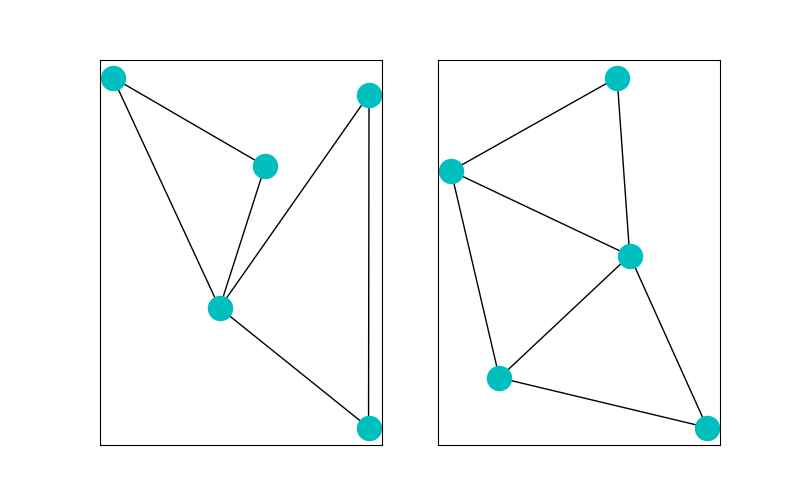
\includegraphics[width=12cm]{Images/H11_T3_evolution.png}
    \centering
    \caption{The possible graphs generated by adding an edge to the $H11$ graph.}
\end{figure}

\begin{table}
    \centering
    \begin{tabular}{||c c c ||} 
    \hline
    Motif Count & Original Motif & Event 1 \\ [0.5ex] 
    \hline\hline
    H3 & 8 & 17 \\ 
    \hline
    H4 & 4 & 6  \\
    \hline
    H5 & 4 & 10 \\
    \hline
    H6 & 0 & 2 \\
    \hline
    H7 & 2 & 3 \\
    \hline
    H8 & 0 & 5 \\
    \hline
    H9 & 0 & 4 \\
    \hline
    H10 & 4 & 6 \\
    \hline
    H11 & 1 & 1 \\
    \hline
    H12 & 0 & 2 \\
    \hline
    H13 & 0 & 0 \\
    \hline
   \end{tabular}
   \caption{Motif counts of the single graph produced by a $T3$ event on the $H11$ motif}
   \label{table:20}
\end{table}

\section{H12}
As we discussed in section 5.10, the $H12$ motifs are not commonly found in the network simulations
because they require a four-walk. In the Thij model, assuming the presence of an $H12$,
one could generate more $H12$'s by a $T2$ event to a vertex of the four-cycle and then a 
$T3$ event to follow. In table ~\ref{table:H13T3} we see even a single $T3$ would suffice to produce two or even four new
$H12$'s.

\begin{figure}
    \includegraphics[width=12cm]{Images/H12_T3_evolution.png}
    \centering
    \caption{The possible graphs generated by adding an edge to the $H12$ graph.}
\end{figure}

\begin{table}
    \centering
    \begin{tabular}{||c c c c||} 
    \hline
    Motif Count & Original Motif & Event 1 & Event 2\\ [0.5ex] 
    \hline\hline
    H3 & 10 & 17 & 18 \\ 
    \hline
    H4 & 2 & 6 & 4 \\
    \hline
    H5 & 2 & 10 & 6\\
    \hline
    H6 & 0 & 2 & 1 \\
    \hline
    H7 & 0 & 3 & 0\\
    \hline
    H8 & 1 & 5 & 4 \\
    \hline
    H9 & 2 & 4 & 8 \\
    \hline
    H10 & 2 & 6 & 6 \\
    \hline
    H11 & 0 & 1 & 0 \\
    \hline
    H12 & 1 & 2 & 4 \\
    \hline
    H13 & 0 & 0 & 0\\
    \hline
   \end{tabular}
   \caption{Motif counts of the possible $T3$ event on the $H12$ motif.}
   \label{table:H13T3}
\end{table}

\section{H13}
The $H13$ does not frequently appear in any of the simulations. $H13$'s
are not readily generated from a $H13$ motif, but require a $T2$ event
and a $T3$ event to connect the newly introduced $T2$ node such that it forms a
$C_4$ at one of the nodes of degree four in the $H13$. Contrast this to an $H7$
or an $H8$ which upon a $T3$ event alone can generate new $H7$'s or $H8$'s. The $H13$
requires events to occur, which are not likely given the attachment mechanism. 

\begin{figure}
    \includegraphics[width=12cm]{Images/H13_T3_evolution.png}
    \centering
    \caption{The possible graph generated by a $T3$ event on the $H13$.}
\end{figure}

\begin{table}
    \centering
    \begin{tabular}{||c c c||} 
    \hline
    Motif Count & Original Motif & Event 1\\ [0.5ex] 
    \hline\hline
    H3 & 18 & 28 \\ 
    \hline
    H4 & 8 & 10 \\
    \hline
    H5 & 12 & 22 \\
    \hline
    H6 & 3 & 8 \\
    \hline
    H7 & 6 & 8 \\
    \hline
    H8 & 6 & 14 \\
    \hline
    H9 & 6 & 12 \\
    \hline
    H10 & 0 & 12 \\
    \hline
    H11 & 0 & 2 \\
    \hline
    H12 & 0 & 6 \\
    \hline
    H13 & 1 & 1\\
    \hline
   \end{tabular}
   \caption{Motif counts of the graph given by a $T3$ event on the $H13$ motif.}
   \label{table:22}
\end{table}


\section{In summary of the $T3$ events}

The $T3$ event is a much more complex animal than the $T2$. For any of the motifs $H3$-$H13$,
 we see how $T3$ events change the motif counts, but 
$T3$'s can add edges \textit{between} different motifs as well as on motifs. If two motifs
are disjoint a $T3$ bridges them and functions as one or more $T2$ events occurring in a single 
time-step. This is still a simple case, but for the eleven motifs considered there are 
fifty-five different possibilities. 

The $T3$ ultimately opens up several possibilities for the model. $C_3$'s and $C_4$'s
are more likely to form around root nodes. We may ultimately see more 
$H6$'s through $H13$'s. For $p=0.2$, the
 Thij model exhibits significantly more clustering throughout time. Shedding light on the impact of the $p$
parameter is for the tools of statistical analysis.


\chapter{Motif Correlation}
Given the analysis in chapters 4 and 5, a $T2$ or $T3$ event applied to a certain motif will generate a given amount of
new motifs. We expect some motifs like $H4$, $H7$, and $H8$ tp correlate together. We
 compute correlation and covariance matrices for the time-series generate by motif counts. There is an order of magnitude difference in covariances between
motifs although all are strongly correlated. All covariance matrices below are described on a log scale.
 We begin with a simulation of the Barabási–Albert model
resulting in the heat maps in figures ~\ref{fig:BAcorr1} and ~\ref{fig:BAcov1}:


\begin{figure}
    \includegraphics[width=10cm]{Images/CorrCoeffpref1.png}\
    \centering
    \caption{Barabási–Albert model with eight initial nodes and $m=1$. The model
     is capable of only producing certain motifs due to the limitations of 
    attaching a single edge and a single node at every time-step. We also see that 
    H7's and H8's correlate together. However, appearances of those motifs depend upon the initialization
     of the graph itself.}
     \label{fig:BAcorr1}
\end{figure}

\begin{figure}
    \includegraphics[width=10cm]{Images/CovMatPref1.png}\
    \centering
    \caption{Barabási–Albert model with eight initial nodes and $m =1$. Here we once again see that 
    the H7 and H8 motifs have a much higher covariance than any other pair of motifs.}
    \label{fig:BAcov1}
\end{figure}


The Barabási–Albert model, for $m=1$, is only capable of generating certain new motifs after the initialization as 
it can only add one edge at a time. Some motifs would require the introduction of an event
which can add edges between existing nodes. The only motifs that increase in size after the initialization
 of the $m=1$ Barabási–Albert model are $H2$,$H4$,$H5$,$H7$, $H8$, $H9$, and $H10$. There is an initialized cluster
of nodes at the center of the graph and new nodes are introduced by the
preferential attachment mechanism. However we see in figures  ~\ref{fig:BA2corr} and ~\ref{fig:BA2coeff} that we can generate all motifs provided
$m>2$.


\begin{figure}
    \includegraphics[width=10cm]{Images/CorrCoeffpref2.png}\
    \centering
    \caption{Barabási–Albert model with three initial nodes and $m=2$. Here we see that all motifs 
    are present. They all have fairly high correlation coefficients, but we see that the H7's and
    H8's are highly correlated as is H7 and H8 with H3.}
    \label{fig:BA2corr}
\end{figure}

\begin{figure}
    \includegraphics[width=10 cm]{Images/CovMatPref2.png}\
    \centering
    \caption{Barabási–Albert model with three initial nodes and $m=2$. The covariance
    offers a different perspective than the correlation figure. We now see that 
    their high covariance between $H7$'s and $H8$'s, and we once again see a relationship
    between $H8$, $H7$, $H3$, $H4$, but many other motifs have a much, much smaller covariances.}
    \label{fig:BA2coeff}
\end{figure}

In figures ~\ref{fig:BA2corr} and ~\ref{fig:BA2coeff}, we have a Barabási–Albert simulation that more so resembles our Thij model for certain parameters. For 
the Barabási–Albert model with $m=2$, all motifs can now be generated via an attachment event.
 This allows for the formation of $C_3$ and $C_4$ subgraphs that are necessary for the
the motifs that also have $C_3$ and $c_4$ subgraphs. We also see that some of our a-priori speculation
in chapter 5 is supported by the correlation and covariance matrices. 


We recall that for relatively high $p$ we are more likely to attach a new node and a new
edge. For relatively low $p$ we attach a new edge between existing nodes. For relatively
high $\lambda$ we are likely to introduce a new message node without any attachments. 
In chapter 4, we discussed that for high $p$ we introduce a new node and attach it with
a the superstar mechanism after selecting a message subgraph with the preferential
attachment mechanism.

\begin{figure}
    \includegraphics[width=10cm]{Images/CorrCoefTwitterModel020209.png}\
    \centering
    \caption{$\lambda=0.2$ and $p=0.2$. We recall low $\lambda$ reduces the chance of only adding a new node (T1)
    and low $p$ reduces the chance of adding a new node and a new edge. Thus 
    probabilistically this simulation should be overall adding only edges between existing nodes.}
\end{figure}

\begin{figure}
    \includegraphics[width=10cm]{Images/CovMatTwitterModel020209.png}\
    \centering
    \caption{$\lambda=0.2$ and $p=0.2$. Here we see once again 
    a strong covariance relationship between $H7$, $H8$, $H9$, $H10$. In this particular graph 
    it's insightful to see these correlate together given these parameters 
    are less likely to produce the induced star subgraph we expect to see for higher $p$.}
\end{figure}

\begin{figure}
    \includegraphics[width=10cm]{Images/CorrCoefTwitterModel020809.png}\
    \centering
    \caption{$\lambda=0.2$ and $p=0.8$. Here in the correlation coefficients we 
    see that there is a strong correlation between $H7$, $H8$, but otherwise a much
    larger spread over the motifs. We also see that no $H6$ or $H13$ motifs appeared
    throughout this simulation.}
\end{figure}

\begin{figure}
    \includegraphics[width=10cm]{Images/CovMatTwitterModel020809.png}\
    \centering
    \caption{$\lambda=0.2$ and $p=0.8$. Here the covariance is relatively 
    very small, except for the H4 variance. This is suggestive of 
    the high $p$ generating that induced star subgraph.}
\end{figure}

\begin{figure}
    \includegraphics[width=10cm]{Images/CorrCoefTwitterModel080209.png}\
    \centering
    \caption{$\lambda=0.8$ and $p=0.2$. Once again we see a familiar structure
    in the correlation matrix. Here though we do see strong correlations 
    across a wider selection of motifs: $C3$, $C4$, $C5$, $H3$, $H4$, $H5$, $H7$, $H8$, $H9$, $H10$. It appears
    the $H6$'s are not easily produced by any of the parameters chosen or the 
    Barabási–Albert model.}
\end{figure}

\begin{figure}
    \includegraphics[width=10cm]{Images/CovMatTwitterModel080209.png}\
    \centering
    \caption{$\lambda=0.8$ and $p=0.2$. We do see strong covariance around the $H4$ with 
    other motifs. There is possibly multiple induced star subgraphs connected that could
    drive this phenomena generating many $H4$'s along with other motifs.}
\end{figure}

\begin{figure}
    \includegraphics[width=10cm]{Images/CorrCoefTwitterModel080809.png}\
    \centering
    \caption{$\lambda=0.8$ and $p=0.8$. Here we have a higher likelihood of adding a new node
     or a new edge and node. Here we do not see any new $H6$'s or $H8$'s produced after the initialization of 
     the graph. Any block structures that we saw in earlier correlation matrices are not as apparent, although
     there is still strong $H7$-$H8$ correlation. }
     \label{fig:corrmat0808}
\end{figure}

\begin{figure}
    \includegraphics[width=10cm]{Images/CovMatTwitterModel080809.png}\
    \centering
    \caption{$\lambda=0.8$ and $p=0.8$. The covariances formed by this simulation suggest once again
    an overlapping of $H4$'s, but there are clearly more nodes attached to the outer edges of this
    induced subgraph. This could lead to the covariance we see between $H3$ and $H4$}
    \label{fig:covmat0808}
\end{figure}

\FloatBarrier

In figures ~\ref{fig:corrmat0808} and ~\ref{fig:covmat0808}, we see clearly evidence of the $S_k$, $k>>1$ induced subgraph
for high values of $p$. We see relatively high covariance between the $H7's$ and
$H8's$ and with $H3$ and $H3$. $H13$ and $H6$ counts don't change at all because the probabilistically
of $T2$ attachment through the superstar mechanism is high relatively high. In fact, this 
mechanism is what encourages the growth of those motifs. We expect to grow in a combinatorial manner
 around $S_k$ induced subgraphs.

\chapter{Dynamic Mode Decomposition}
In addition to using statistical methods we can view the motif counts through the lens of dynamical systems. We achieve this through
dynamic mode decomposition to find the modes and eigenvalues of the Koopman operator.
 The DMD algorithm produces spatiotemporal coherent structures (modes)
which have associated temporal behavior: growth, decay, and oscillation. 

\section{The Koopman Operator}
Suppose we have some continuous, finite-dimensional, non-linear dynamical system 

$$
\frac{dy}{dt} = f(y) \quad y(0) = x \in \mathbb{R}^N
$$

\noindent with $N>>1$. $y(t)$ is the state of the dynamical system at time $t$. Sampling the dynamical
system every $\Delta t$ we get the discrete time-series

$$
y_{k+1} = F(y_k).
$$

\noindent with $y_k = y(t_k) = y(k \Delta t)$. We would like a coordinate transformation render the dynamics of the
 non-linear system much simpler. In this new coordinate system the dynamics could be
described linearly. We seek some $\phi$ such
that $z = \phi(y)$ where the dynamics are much easier to evaluate in the
 z-coordinates. In this context, we seek $y_{k+1} = Ky_k$.


 \noindent We define a Hilbert space of observables, that is 

$$
L_2(O) = L_2(\mathbb{R}^N, \mathbb{R}, \mu),
$$

\noindent with an associated norm 

$$
\int_{\mathbb{R}^N} |g(x) |^2 d\mu(x)  < \infty,
$$

\noindent where $\mu$ is some appropriately chosen measure. The Koopman
operator $K$ is a mapping between the Hilbert space of observables unto itself,

$$
K: L_2(O) \rightarrow L_2(O)
$$

\noindent such that

$$
Kg(x) = g(F(x)) = g(x_{k+1}) \quad g \in L_2(O)
$$

\noindent For an eigenfunction $\varphi$ of $K$ and their associated eigenvalue $\mu$ we have that 


$$
K(\varphi(x_k)) = \mu \varphi(x_k) = \varphi(x_{k+1})
$$

\noindent A vector of observables $g$ can be written in terms of a basis of eigenvectors

$$
g(x_{k}) = \sum^{\infty}_{j=1}\varphi_j(x_k) \xi_j
$$

\noindent which implies we can evolve the system like so

$$
g(x_{k+1}) = \sum^{\infty}_{k=1} \mu_j \varphi_j(x_k) \xi_j.
$$

\noindent However, finding the exact eigenfunctions, modes, and eigenvalues of $K$ analytically
is difficult for any meaningful problem, and thus we have to resort to
numerics to estimate them via the Dynamic Mode Decomposition.


\section{Approximating the Koopman Operator via Dynamic Mode Decomposition}
Similar to the previous section we consider now sampled-data collected from a non-linear dynamical system
of the form:

$$
\frac{dx}{dt} = f(x,t; \mu)
$$

\noindent where $x(t)\in \mathbb{R}^{n}$ is a vector representing the state of the dynamical system
at time $t$ and $\mu$ are parameter values.
 Our data is sampled at discrete points in time every $\Delta t$. Every sampling can be written as $x_{k} = x(k \Delta t)$. This 
discrete time-flow map we denote $X_{k+1} = F(x_k)$. \
We can then extend our collected data:

$$
y_k = g(x_k)
$$

\noindent where $g(k)$ is the set of observables formed from the state space. 
Here we now use the Koopman operator theory to introduce a
 linear, infinite-dimensional operator $A$:

$$
A g = A g(x_k) = g(x_{k+1}),
$$
\noindent exactly as we described in section 8.1. $A$ advances measurements along the flow $F$ by $\Delta t$.
We calculate the Koopman operator of our dynamical system in the following manner \cite{brunton2021modern}.
Beginning with our data snapshot matrix composed of the relevant observables we write

$$
G = [g(x_0), g(x_1), g(x_2), \dots ,g(x_n)] = [g_1,g_2,\dots, g_n],
$$

\noindent which we can then break into two matrices:

\begin{align*}
    & G_+ = [g_1, g_2, g_3, \dots g_n]\\
    & G_- = [g_0, g_1, g_2, \dots g_{n-1}]\\\
\end{align*}

\noindent The matrix $G_+$ is simply our matrix $G_-$ taken forward one step in time. 
The particular Koopman operator ${A}$ we wish to find, satisfies:

$$
G_+ = AG_-
$$

\noindent Subtracting $AG_-$ from both sides, we have

$$
G_+ - {A}G_- = 0
$$

\noindent We would then like to find that 

$$
{\tilde A} = {\argmin_{A}} \|G_+ - {A}G_- \|_{F}
$$

\noindent where $\| \|_{F}$ denotes the Frobenius norm. We still have the matter of finding the 
${\tilde A}$ that minimizes the norm, which is our best approximation to $A$. We could
use a least-squares fit or solve using Moore pseudo-inverse calculating $G_+G^{\dagger}_-$, but we instead
 make use of the r-rank singular value decomposition in the following way.

\begin{align*}
    G_+ &= {\tilde A}G_- \\
    &= {\tilde A}U_rS_rV^{T}_r \quad \text{by singular value decomposition} \\ 
G_+ V_r S^{-1}_r U^{T}_r &= {\tilde A} \\
\end{align*}

Taking the $r$-rank of the SVD limits the number of modes and
 eigenvalues to a few that satisfy a threshold tolerance giving us a low-rank model
 that still captures most of the information. 
The columns of $U$ are the Proper Orthogonal Decomposition modes of the
 data. The associated singular values are normalized by their total.
The singular values act as weights and can be used to discard those
 modes which don't contribute a substantial amount of energy in the decomposition.

Finally, we use an eigendecomposition on the left-hand side to find the 
eigenvalues and associated modes of $A$, our Koopman modes. Once we have the Koopman modes and eigenvalues, we can begin to look at which DMD modes
"contribute the most" throughout the snapshot matrix and the associated eigenvalues which describe
their temporal behavior: growth, decay, or oscillation. We have not yet
 discussed how to choose $g$, how we build our dictionary of observables. If we choose $g$ to 
be the identity mapping, then the method reduces to the standard DMD algorithm, where $g(x_i) = x_i$.
Choosing any other function of $g$ in a meaningful way requires some a-priori knowledge of the system.
A mapping $g$ can extend the dictionary of observables beyond the state space using some appropriate 
basis, usually a Taylor or Fourier basis. This is aptly called Extended Dynamic Mode Decomposition (EDMD) \cite{doi:10.1137/1.9781611974508}. A quick example of such
a choice might be:

$$
Y = \{y_1, y_2, y_3, \dots, y_n  \}, \quad y_i \in \mathbb{R}^{N}
$$

\noindent with 

$$
y_i = {y_{i,1}, y_{i,2},\dots, y_{i,N}} 
$$

\noindent then we might take $g$ such that:

$$
G(Y) = \{g(y_1), g(y_2), g(y_3), g(y_4), \dots , g(y_n)\}
$$

$$
g(y_i) = {y_{i,1}, y_{i,2},\dots, y_{i,N}, y^{2}_{i,1}, y_{i,1}y_{i,2}, \dots, y^{2}_{i,N}} 
$$

\noindent This example of $g$ is one of many possible functions.

\section{Kernel Dynamic Mode Decomposition}

EDMD can quickly generate a large set of observables
 and the computational complexity of the problem increases rapidly. It suffers from the
 dimensionality problem and works well provided many more snapshots than state-space
variables. If one is analyzing, for instance, n-dimensional fluid flows, the flattened matrix-snapshot
can easily have thousand of entries. Extending the state-space by building a dictionary with nonlinear combinations of the 
state space will generate very large matrices \cite{williams2015kernelbased}. For that reason, one applies the kernel trick. Instead of evaluating
the high dimensional state space directly, one can take inner-products of the state space using kernel functions
to ''collapse" the information of many nonlinear terms to a single value. In our analysis, our vectors are relatively small and thus not a conventional use of KDMD. 
 KDMD still offers a way to analyze nonlinear terms through the kernel trick and as we will see in chapters 9, can produce 
 Koopman modes with relatively low mode error. 
 These modes, but not their associated eigenfunctions, are similar in structure to the one's produced by DMD, but not identitical \cite{doi:10.1137/1.9781611974508}. 
We introduce the notion of the kernel.

\begin{dfn}
    We define the Kernel function $k:\mathbb{R}^n X \mathbb{R}^n \rightarrow \mathbb{R}, \quad k(x,{\hat x}) = \langle \phi(x), \phi({\hat x})\rangle$.
     That is $k$ maps a pair of vectors to an inner product of observables of the data.
\end{dfn}

\noindent There are a variety of different kernels that we may choose. Some include:

\vspace{3mm}

\noindent Sigmoid:
$$
f(x,x') = \text{tanh}(x^Tx' + a)
$$

\vspace{3mm}

\noindent Radial: 

$$
f(x,x') = e^{-a|x-x'|^2}
$$

\vspace{3mm}


\noindent Polynomial:

$$
f(x,x') = (1 + x^Tx')^p
$$

\vspace{3mm}

As mentioned, the kernel functions allow us to store a large amount of information in a single value. We generate matrices
$\Phi^+$ and $\Phi^-$ from the polynomial basis function. Our data snapshots are as
follows:

$$
 Y = \{y_1,y_2,y_3, \dots y_n\}
$$

$$
k (y,{\hat y}) = (1 + y^T {\hat y})^p
$$

\noindent We then construct the observable matrices $\Phi^{+}\in \mathbb{C}^{n \times n}$ and $ \Phi^{-}\Phi^{+}\in \mathbb{C}^{n \times n}$.

$$
\Phi^{+}_{i,j} = k(Y^{+}_{i}, Y^{-}_j)
$$

$$
\Phi^{-}_{i,j} = k(Y^{-}_{i}, Y^{-}_j)
$$

\noindent Then, for every element in $\Phi^{+}_{i,j}$ and $\Phi^{-}_{i,j}$, we have a kernel between two snapshots in time. The dimensionality of the
extended observables is not constrained by the total number of snapshots. For KDMD, we finally get
our approximations to the Koopman modes by applying the SVD and using matrix multiplication to find our approximation to the matrix $A$.

$$
\Phi^{+} = {\bar A} \Phi^{-}
$$

\section{Accuracy Criterion}
For the DMD and KDMD algorithms, we evaluate how
well the methods performed. We consider two different measures
of accuracy. First, we define the one-step reconstruction
error $r$. We define the matrix ${\tilde G}$ where the j'th column vectors of ${\tilde G}$ are the one-step
reconstructions of the state space at time $j+1$ for $j=0,1,\dots, n-1$.

$$
{\tilde G}_{j} = \sum_{i} \mu_i b_{i,j} \xi_i
$$

$$
r = \frac{\|G_{+} - {\tilde G} \|_F}{\|G_{+}\|_F}
$$

\noindent where $\| \cdot \|_F$ denotes the Frobenius norm.

We also wish to know if the approximated modes and eigenvalues are good approximations to 
Koopman modes. We define the Rowley criterion \cite{zhang2017evaluating}. Let $\xi_j$ and $\mu$ be a Koopman mode for the
 dynamical system $F$ and its corresponding eigenvalue. Provided that $\xi_j$ and $\mu_j$ are
a true eigenpair it follows:

$$
\xi_j \circ F = \mu_j \xi_j
$$

\noindent Now, letting $\|\cdot\|$ denote the $L2$ norm, we would like to calculate 

$$
\frac{\| \xi \circ F - \mu \xi \|}{\| \xi \|}
$$

\noindent However, if we know $F$ then DMD isn't a useful tool.
We must estimate $F$ using a finite number of data points. We take
two data points $x_k, x_{k+1} \in X$. We can now write 

$$
{\tilde r}_{j} = \frac{\sum_{k} |\varphi_j(x_{k+1}) - \mu_j \varphi_j(x_{k})|}{\sum_{k} |\varphi_j(x_k )|}
$$

This equation measures how much each eigenfunction $\phi_j$ behaves like a Koopman eigenfunction. We can use 
this to evaluate each mode individually and could potentially use it to select modes for low-rank reconstruction \cite{zhang2017evaluating}. If ${{\tilde r}_j}$ is close to one
the eigenpair is unreliable, because the difference in the eigenpair is of the same magnitude of the eigenfunction. Therefore a 
good eigenpair with have a mode error of $0< {{\tilde r}_j} \ll 1$.

\chapter{Results}

\section{Preprocessing Data}
Dynamic Mode Decomposition is sensitive to
 noise in the data. We implement several techniques to better the errors of the DMD modes.
  First, we modify the data via a Poisson process such that the events do not occur at each
snapshot, but events occur relative to a $\delta t$. Suppose we have 

$$
X = [x_1,x_2,x_3,\dots, x_n]
$$

\noindent where $x_i$ describes is a feature vector at $i \Delta t = t$. We then allow

$$
A = \frac{1}{2} \left( \frac{1}{\lambda} +  \psi(x;\lambda) \right), \quad \psi(x;\lambda) = \lambda e^{-\lambda x}
$$

$$
\delta t = \min(A)
$$

 $\psi(x;\lambda)$ is an exponential probability distribution from which we draw a thousand samples with $\lambda=10$.
  We then distribute events in the following
way. Let ${\hat A}$ denote a matrix that initially only contains the value $x_1$. For $k=1,2,3,\dots$ we calculate $k \delta t$. While $k\delta t < A_i$ we append $x_i$ to 
a ${\hat A}$. Thus we generate a new matrix ${\hat A}$ that now contains $n = \sum^{N}_{i=1} A_i \mod(\delta t)$ 
${\hat A}$. This distributes the events according to a Poisson process. After we distribute events in tome according to this process, we
 smooth the data with the window-average. This smoothing will help the DMD and KDMD generate better fits. Last, we center the data about its mean to improve the fit.

\section{DMD: Barabási–Albert m=1}
We now reach the results of the DMD algorithm applied to the
motif counts of the simulated networks. We will first examine DMD applied to the 
Barabási–Albert motif counts. Thereafter, we examine several parameter choices for the Thij model.
For all DMD and KDMD results, the Koopman modes
 and eigenvalues are as discussed in chapter 8. The phi modes are simply the weighting of each Koopman mode 
 at each time step. These tell us how much energy the respective Koopman mode contributes at a given time
step.

We can now consider DMD results of the Barabási–Albert motif counts. We show in this section
the $m=1$ and $m=2$ case to observe differences and similarities between the approximated 
Koopman modes and eigenvalues. 

For the $m=1$ case, we know that a new node and edge are added at every time step. Moreover from our
correlation and covariance heat maps, we know the only motifs that change in the $m=1$ case 
are as such: 

\newpage

\begin{figure*}
    \includegraphics[width=17cm]{Images/smooth_pref_counts_1.png}
    \centering
    \caption{Smooth motif counts for Barabási–Albert model $k=1$.}
\end{figure*}
\clearpage

\begin{figure*}
    \includegraphics[width=14cm]{Images/DMDm1k300eigen-1.png}
    \centering
    \caption{Mode Eigenvalues for Barabási–Albert model
    with $k=1$.}
\end{figure*}

\begin{figure*}
    \includegraphics[width=12cm]{Images/DMDm1k300eigen-2.png}
    \centering
    \caption{Koopman modes by DMD for Barabási–Albert model
    with $k=1$.}
\end{figure*}

\clearpage

\section{KDMD: Barabási-Albert m=1}

We now examine the same simulations through the KDMD method.

\FloatBarrier

\begin{figure*}
    \includegraphics[width=14cm]{Images/KDMDm1k300eigen-1.png}
    \centering
    \caption{Mode Eigenvalues by KDMD for Barabási–Albert model
    with $k=1$.}
\end{figure*}

\begin{figure*}
    \includegraphics[width=12cm]{Images/KDMDm1k300eigen-2.png}
    \centering
    \caption{Koopman modes by KDMD for Barabási–Albert model
    with $k=1$.}
\end{figure*}

\clearpage

\FloatBarrier

\section{DMD: Barabási–Albert m=2}

\begin{figure*}
    \includegraphics[width=17cm]{Images/smooth_pref_counts_2.png}
    \centering
    \caption{Smooth motif counts for the Barabási–Albert model with $k=2$.}
\end{figure*}

\clearpage
\begin{figure*}
    \includegraphics[width=14cm]{Images/DMDm2k300eigen-1.png}
    \centering
    \caption{Koopman modes by DMD for the Barabási–Albert model
    with $k=2$.}
\end{figure*}

\begin{figure*}
    \includegraphics[width=12cm]{Images/DMDm2k300eigen-2.png}
    \centering
    \caption{Koopman Modes by DMD for the Barabási–Albert model
    with $k=2$.}
\end{figure*}

\clearpage

\section{KDMD: Barabási–Albert m=2}

\begin{figure*}
    \includegraphics[width=14cm]{Images/KDMDm2k300eigen-1.png}
    \centering
    \caption{Mode eigenvalues by KDMD for the Barabási–Albert model
    with $k=2$.}
\end{figure*}

\begin{figure*}
    \includegraphics[width=12cm]{Images/KDMDm2k300eigen-2.png}
    \centering
    \caption{Koopman modes by KDMD for the Barabási–Albert model
    with $k=2$.}
\end{figure*}

\clearpage

\section{DMD: Thij Model with $\lambda=0.2$, $p=0.2$}
\begin{figure*}
    \includegraphics[width=17cm]{Images/smooth_twitter_counts_020209.png}
    \centering
    \caption{Smooth motif counts for the Thij model
    with $\lambda=0.2$, $p=0.2$.}
    \label{fig:pthij0202}
\end{figure*}

\clearpage

\begin{figure*}
    \includegraphics[width=14cm]{Images/DMD_twitter_020209-1.png}
    \centering
    \caption{Mode eigenvalues by DMD for the Thij model
    with $\lambda=0.2$, $p=0.2$.}
\end{figure*}

\begin{figure*}
    \includegraphics[width=12cm]{Images/DMD_twitter_020209-2.png}
    \centering
    \caption{Koopman Modes by DMD for the Thij model
    with $\lambda=0.2$, $p=0.2$.}
\end{figure*}

\clearpage

\section{KDMD: Thij Model with $\lambda=0.2$, $p=0.2$}

\FloatBarrier


\begin{figure*}
    \includegraphics[width=14cm]{Images/KDMD_twitter_020209-1.png}
    \centering
    \caption{Mode eigenvalues by KDMD for the Thij model
    with $\lambda=0.2$, $p=0.2$.}
\end{figure*}

\begin{figure*}
    \includegraphics[width=12cm]{Images/KDMD_twitter_020209-2.png}
    \centering
    \caption{Koopman modes by KDMD for the Thij model
    with $\lambda=0.2$, $p=0.2$.}
\end{figure*}

\clearpage
\FloatBarrier
\section{DMD: Thij Model with $\lambda=0.2$, $p=0.8$}
\begin{figure*}
    \includegraphics[width=17cm]{Images/smooth_twitter_counts_020809.png}
    \centering
    \caption{Motif counts for the Thij model with $\lambda=0.2$, $p=0.8$.}
    \label{fig:pthij0208}
\end{figure*}

\clearpage
\begin{figure*}
    \includegraphics[width=14cm]{Images/DMD_twitter_020809-1.png}
    \centering
    \caption{Mode eigenvalues by DMD for the Thij model
    with $\lambda=0.2$, $p=0.8$.}
    \label{fig:dmd02081}
\end{figure*}

\begin{figure*}
    \includegraphics[width=12cm]{Images/DMD_twitter_020809-2.png}
    \centering
    \caption{Koopman modes by DMD for the Thij model
    with $\lambda=0.2$, $p=0.8$.}
    \label{fig:dmd02082}
\end{figure*}

\clearpage
\section{KDMD: Thij Model with $\lambda=0.2$, $p=0.8$}


\begin{figure*}
    \includegraphics[width=14cm]{Images/KDMD_twitter_020809-1.png}
    \centering
    \caption{Mode eigenvalues by KDMD for the Thij model
    with $\lambda=0.2$, $p=0.8$.}
    \label{fig:kdmd02083}
\end{figure*}

\begin{figure*}
    \includegraphics[width= 12cm]{Images/KDMD_twitter_020809-2.png}
    \centering
    \caption{ Koopman modes by KDMD for the Thij model
    with $\lambda=0.2$, $p=0.8$.}
    \label{fig:kdmd02084}
\end{figure*}

\FloatBarrier

\clearpage

\section{DMD: Thij Model with $\lambda=0.8$, $p=0.2$}
\begin{figure*}
    \includegraphics[width=17cm]{Images/smooth_twitter_counts_080209.png}
    \centering
    \caption{Motif counts for the Thij simulation with $\lambda=0.8$, $p=0.2$}
    \label{fig:pthij0802}
\end{figure*}

\clearpage
\begin{figure*}
    \includegraphics[width=14cm]{Images/DMD_twitter_080209-1.png}
    \centering
    \caption{Mode eigenvalues by DMD for the Thij model
    with $\lambda=0.8$, $p=0.2$.}
\end{figure*}

\begin{figure*}
    \includegraphics[width=12cm]{Images/DMD_twitter_080209-2.png}
    \centering
    \caption{Koopman modes and phi modes by DMD for the Thij model
    with $\lambda=0.8$, $p=0.2$.}
\end{figure*}


\clearpage
\section{KDMD: Thij Model with $\lambda=0.8$, $p=0.2$}


\begin{figure*}
    \includegraphics[width=14cm]{Images/KDMD_twitter_080209-1.png}
    \centering
    \caption{Mode eigenvalues by KDMD for the Thij model
    with $\lambda=0.8$, $p=0.2$.}
\end{figure*}

\begin{figure*}
    \includegraphics[width=12cm]{Images/KDMD_twitter_080209-2.png}
    \centering
    \caption{Koopman modes and phi modes by KDMD for the Thij model
    with $\lambda=0.8$, $p=0.2$.}
\end{figure*}

\FloatBarrier

\clearpage

\section{DMD: Thij Model with $\lambda=0.8$, $p=0.8$}
\begin{figure*}
    \includegraphics[width=17cm]{Images/smooth_twitter_counts_080809.png}
    \centering
    \caption{Motif counts for the Thij model with $\lambda=0.8$, $p=0.8$.}
    \label{fig:pthij0808}
\end{figure*}

\clearpage

\begin{figure*}
    \includegraphics[width=14cm]{Images/DMD_twitter_080809-1.png}
    \centering
    \caption{Mode eigenvalues by DMD for the Thij model
    with $\lambda=0.8$, $p=0.8$.}
    \label{fig:dmd08081}
\end{figure*}

\begin{figure*}
    \includegraphics[width=12cm]{Images/DMD_twitter_080809-2.png}
    \centering
    \caption{Koopman modes by DMD for the Thij model
    with $\lambda=0.8$, $p=0.8$.}
    \label{fig:dmd08082}
\end{figure*}

\clearpage
\section{KDMD: Thij Model with $\lambda=0.8$, $p=0.8$}

\begin{figure*}
    \includegraphics[width=14cm]{Images/KDMD_twitter_080809-1.png}
    \centering
    \caption{Mode eigenvalues by KDMD for the Thij model
    with $\lambda=0.8$, $p=0.8$.}
    \label{fig:dmd08083}
\end{figure*}

\begin{figure*}
    \includegraphics[width=12cm]{Images/KDMD_twitter_080809-2.png}
    \centering
    \caption{Koopman modes and phi modes by KDMD for the Thij model
    with $\lambda=0.8$, $p=0.8$.}
    \label{fig:dmd08084}
\end{figure*}

\FloatBarrier
\clearpage

\section{Accuracy of Methods}

We want to know how DMD handles different parameter simulations of the Thij model and how it compares to KDMD.
 We also need to evaluate how the two accuracy criterion described in section 8.2 perform across
simulations and methods. We recall that we use the one-step reconstruction error, a measure of 
how well the modes and eigenvalues replicate the data. We also defined the mode error describing how 
well each DMD mode behaves like a Koopman mode. We begin with the
reconstruction error of the Barabási–Albert models.

\begin{figure}
    \includegraphics[width=14cm]{Images/pref_rec_errors.png}
    \centering
    \caption{In orange have the reconstruction error of the DMD results and in cyan 
    the KDMD results. The DMD performs much better with regard to reconstruction error, by several scales of magnitude.}
    \label{fig:prefrecerror}
\end{figure} 

\begin{figure}
    \includegraphics[width=14cm]{Images/Pref_Mode_errors.png}
    \centering
    \caption{DMD also seems to produce modes with lower mode error. The scale on this figure is linear,
    so the differences are not as stark in figure~\ref{fig:prefrecerror}. The KDMD method for $m=1$
    does seem to perform comparable given that all the modes in KDMD have dynamic behavior.}
\end{figure} 

% \begin{table}
%     \centering
%     \begin{tabular}{||c c c ||} 
%     \hline
%     Params & DMD & KDMD  \\ [0.5ex] 
%     \hline\hline
%     $k=1$ & 1.73e-04 & 9.23e-01\\ 
%     \hline
%     $k=2$ & 2.02e-04 &  1.42e+00 \\
%     \hline
%    \end{tabular}
%    \caption{One-step Errors of the DMD and KDMD methods on the Barabási–Albert model with $k=1$ and $k=2$}
%    \label{table:15}
% \end{table}

% \begin{figure}
%     \includegraphics[width=8cm]{Images/mode_error_dmd_prefattach1.png}
%     \centering
%     \caption{DMD mode error for preferential attachment with $k=1$}
% \end{figure}

% \begin{figure}
%     \includegraphics[width=8cm]{Images/mode_error_kdmd_prefattach1.png}
%     \centering
%     \caption{KDMD mode error for preferential attachment with $k=1$}
% \end{figure}

% \begin{figure}
%     \includegraphics[width=8cm]{Images/mode_error_dmd_prefattach2.png}
%     \centering
%     \caption{KDMD mode error for preferential attachment with $k=2$}
% \end{figure}

% \begin{figure}
%     \includegraphics[width=8cm]{Images/mode_error_kdmd_prefattach2.png}
%     \centering
%     \caption{KDMD mode error for preferential attachment with $k=2$}
% \end{figure}

\FloatBarrier

Now we consider the performance of DMD and KDMD on the more complex Thij model.

% \begin{table}
%     \centering
%     \begin{tabular}{||c c c ||} 
%     \hline
%     $(\lambda,p)$ & DMD & KDMD  \\ [0.5ex] 
%     \hline\hline
%     $(0.2,0.2)$ & 4.71e-05 &  7.61e-02\\ 
%     \hline
%     $(0.2,0.8)$ & 2.59e-04 & 3.35e-01\\
%     \hline
%     $(0.8,0.2)$ & 1.31e-04 & 1.17e-01\\
%     \hline
%     $(0.8,0.8)$ & 2.48e-04 &  1.95e-01 \\
%     \hline
%    \end{tabular}
%    \caption{One-step errors of the DMD and KDMD methods on the Thij model.
%    DMD generally performs better than KDMD in reconstruction errors.}
%    \label{table:15}
% \end{table}

\begin{figure}
    \includegraphics[width=14cm]{Images/rec_errors.png}
    \centering
    \caption{DMD and KDMD reconstruction errors across Thij simulations. DMD here again
    has very low reconstruction errors compared to KDMD.}
\end{figure}

Now we can evaluate the respective mode errors.

\begin{figure}
    \includegraphics[width=14cm]{Images/Mode_errors.png}
    \centering
    \caption{DMD and KDMD mode errors across simulations. DMD does seem to produce 
    better results, but KDMD has the advantage of being able to produce more Koopman modes. The
    KDMD results for $\lambda=0.2$, $p=0.2$ is a noticable outlier with very low mode error.}
\end{figure}

\FloatBarrier

Examining these mode errors, we can see the modes
from the standard DMD algorithm are just as accurate or more 
 accurate than the KDMD modes. DMD also performs much better in terms of one-step
reconstruction error over KDMD, which is not unexpected since 
DMD is a least-squares fit to the data. Overall the KDMD modes look to 
be good Koopman modes. However, examining the phi modes above we see that in 
DMD we can pick out modes which effectively contribute more to the overall energy 
at each time step \cite{chris}. We could use to select a low rank representation
of the data, reconstructing it with only a few nodes. However, reconstruction is not the focus 
of this thesis.


\chapter{Discussion}
From the results in the previous chapter, we are able to sift out differences in dynamic behavior by applying
 DMD to the motif counts. DMD produces modes that have associated temporal
patterns: growth, decay, and oscillation. For many of these simulations, the real part of
 the approximated Koopman eigenvalues clusters around one or zero. We only see zero eigenvalues
given that a mode does not exhibit any temporal behavior such as in the $k=1$ Barabási–Albert 
simulation or the $p=0.8$ Thij simulations. Otherwise our observed eigenvalues tend to cluster
in tight groups at the edge of the unit circle. 

Examining the modes above we see block structure in the heatmaps in a pattern similar to those 
generated in the correlation and covariance matrices in chapter 7. If we look to 
figure~\ref{fig:dmd02082} and ~\ref{fig:kdmd02084} we can pick out in the former the strongest
DMD modes reflect an association between $H3$, $H4$, $H7$, $H8$. In the latter simulation, KDMD produces
modes of equal amplitude throughout time but we can once again see the association between the same motifs. 

For certain simulations, we have a readily available a-priori explanation
of global network dynamics, the formation of large induced star subgraphs. The preferential
attachment mechanism effectively acts as a positive feedback loop - the
additional attachment of nodes to a node $u$ increases
the likelihood of the future attachment to node $u$. Even without 
 such a tale DMD and KDMD are capable of extracting out underlying 
structure from those simulations, for example a Thij model with $\lambda=0.8$, $p=0.2$ or $\lambda=0.8$, $p=0.8$.

This tale of induced star subgraphs on the network is most apt when
there is a strong preferential attachment mechanism, but not so for $T3$ events.
 It's true that for any of the given simulations examined, the $H4$ motif was present if not outright
central to the formation of the network's temporal development. The development
of other motifs alongside the $H4$ development depends on the initialization
of the graph, especially in the Barabási–Albert model which cannot add in
edges between any two nodes. Even for the Barabási–Albert simulations in chapter 5 
we see that $H4$ is preparing to surpass in either the $m=2$ or $m=1$
simulations. One might speculate, asymptotically, given a preferential attachment
mechanism a network, $H4$ will come to be the dominant motif.

This is further motivated by our analysis of the correlation and covariance
matrices of the given simulations. The $H7$'s and $H8$'s generally have 
relatively high covariances with one another and relatively high variances.
In the analysis of their development, adding a node and an edge to either of the
motifs generates a host of new ones either combinatorially or multiplicatively 
respectively. 

\chapter{Conclusion}

The motif counts make valuable features to characterize the local structure 
of the network over time. Their dynamical behavior can be studied using
traditional statistical methods as we have done above using correlation
and covariance statistics. However DMD also provides a way to extract 
the spatiotemporal coherent structures associated with the motif counts. It 
is a different way of understanding how attaching nodes and edges to a graph,
generates those new motifs. 

The effects of adding nodes and edges can be understood through graph theory. As
the attachment mechanisms become more complex the analysis becomes much more
difficult. The connection of disjoin graphs can generate many new motifs quite
suddenly. In the simplest case however the induced star subgraph offers 
a good explanation of why motifs correlate the way they do and could 
offer a way to interpret the DMD modes in the future.The study 
of motifs is young and better understanding of the dynamic interactions 
between motifs would greatly improve the ability to interpret the modes as physical
phenomena. 

The models above can be made more complex by introducing other mechanisms, such as An
edge deletion mechanism. That mechansim would cause the deletion of certain motifs and 
could potentially introudice oscillatory behavior into the motif counts. These
DMD and KDMD modes may offer context to the modes we see above in chapter 8. 


